    \documentclass[a4paper,12pt,twoside]{ThesisStyle}
\usepackage[utf8]{inputenc}
\usepackage{thesis-style}
\usepackage[english]{babel}
\usepackage[T1]{fontenc}

\usepackage{subcaption}
\usepackage{graphicx}
\usepackage{enumitem} % Required for customizing itemize labels
\usepackage{enumitem}
\usepackage{fancyvrb}
\usepackage[toc,page]{appendix}
\usepackage{adjustbox}
\usepackage{pdflscape}
\usepackage{booktabs}% http://ctan.org/pkg/booktabs



\usepackage[table]{xcolor}
\definecolor{signaturegray}{gray}{0.98}

\RequirePackage{tikz}
\definecolor{ao}{rgb}{0.0, 0.5, 0.0}
\definecolor{darkpastelgreen}{rgb}{0.01, 0.75, 0.24}
\definecolor{amber}{rgb}{1.0, 0.75, 0.0}
\usetikzlibrary{mindmap}  % Mindmap drawing library

\setlength{\parindent}{0pt} % Drops all identation of all paragraphs

\begin{document}

\frontmatter

\pagenumbering{gobble}

\thispagestyle{empty}
\begin{table}[htb]
\centering
\begin{Large}
\resizebox{\textwidth}{!}{\begin{tabular}{ | l |}
 \hline
 \\

\includegraphics[scale=0.9]{imatges/logo_eps.png} \\[0.7cm]
\centerline{Treball Final de Màster}\\[1cm]
\hline
\\
Estudi: Màster en Ciència de Dades\\[0.7cm]
\hline
\\
Títol: Una Plataforma per Classificar Melanomes \\[0.7cm]
\hline
\\
Document: Memòria\\[0.7cm]
\hline
\\
Alumne: Wilber Eduardo Bermeo Quito \\[0.7cm]
\hline
\\
Tutor: Rafael Garcia Campos \\
Departament:  ARQUITECTURA I TECNOLOGIA DE COMPUTADORS \\
Àrea: ARQUITECTURA I TECNOLOGIA DE COMPUTADORS \\[0.7cm]
\hline
\\
Convocatòria (mes/any): Setembre 2022\\[0.7cm]
\hline

\end{tabular}}
\end{Large}
\end{table}

\newpage
\hypersetup{pageanchor=false}
\begin{titlepage}

% Upper part of the page

\includegraphics[scale=0.9]{imatges/logo_eps.png} \\[1cm]
\begin{center}
\textsc{\Large Master's thesis} \\[1cm]

% Title
\begin{spacing}{2}
\HRule \\
\textbf{\Huge A Platform for Classifying Melanoma} \\
\HRule \\[0.5cm]
\end{spacing}

% Author and supervisor and other data
{
\large
\textsc{Wilber Eduardo Bermeo Quito} \\
\small{September 2022} \\[0.75cm]
Master in Data Science \\[0.75cm]
\emph{Advisors:} \\[0.1cm]
\large
\textsc{Dr. Rafael Garcia Campos} \\
\small{Universitat de Girona} \\
\small{Departament of Computer Architecture and Technology} \\[0.5cm]

\large
\textsc{Sr. Luis Pla Llopis} \\
\small{Accenture S.L.} \\

}

\end{center}
\end{titlepage}
\hypersetup{pageanchor=true}

\titlepage

%\dominitoc


\pagenumbering{roman}

\begin{abstract}
  We present a platform for Melanoma Classification, leveraging a technical
  infrastructure based on Convolution Neural Network (CNN) models based on
  ResNet18.

  For training and validation, exclusively we have utilized image data, and no
  additional metadata is incorporated during the training process. Various
  training strategies, such as data augmentation, learning rate decay, dropout,
  etc., were employed to enhance models performance.

  The resulting models are accessible through a  API, enabling users to
  interact with them via a straightforward web application. Users can submit
  batches of images to the API for classification, contributing to a
  user-friendly experience.

  This platform demonstrates the efficacy of CNNs in melanoma classification,
  highlighting the importance of diverse training approaches. The API provides
  a practical interface for users to seamlessly integrate melanoma
  classification into their workflows.
\end{abstract}


\section{Introduction}

Skin cancer, including melanoma, is a significant global public health concern.
Melanoma presents a considerable challenge due to its high mortality rate and
the critical importance of early detection for successful treatment. Cancer
begins when healthy cells undergo changes that cause them to grow and divide
uncontrollably, forming tumors. These tumors can be classified as either
cancerous (malignant) or non-cancerous (benign). \\

In recent times, there has been a growing focus on automating tasks in the
medical field through Computer-Aided Diagnosis (CAD)\footnote{CAD refers to the
use of computer algorithms and technologies to assist healthcare professionals
in the process of medical diagnosis.}. Some studies have demonstrated that
these systems can achieve results similar to those of professionals. However,
the integration of CAD into the medical system remains a significant challenge. \\

The development of a CAD system necessitates the creation of models capable of
effectively classifying melanoma. The SIIM-ISIC Melanoma Classification
challenge specifically tasks participants with building models for identifying
melanoma using skin lesion images and associated metadata. This thesis outlines
our approach, wherein we leverage data from this challenge to train our models
and subsequently expose them through our platform. By doing so, we contribute
to the ongoing efforts to bridge the gap between cutting-edge medical imaging
technology and practical clinical applications.

\newpage

\section{Objectives}

The final objective of this thesis is to craft a CAD infrastructure,
focused on melanoma detection using deep learning vision models capable of detecting melanoma on dermoscopy images. To this end, the gradual achievements that
must be accomplished are:

\begin{itemize}

  \item Gaining a comprehensive understanding of the theory
    behind deep learning vision models and its practical applications.

   \item Select a base transfer model. Is the model good enough?, the selection of this model is given by the technical limitations?, or any other justification.

  \item Study different approaches to train the models and select a good  evaluate metric given the dataset distribution of dermoscopy images.

  \item  Develop the CAD infrastructure. It should contain
    the  trained models, a simple web UI\footnote{User Interface. Is
    the point of human-computer interaction and communication in a device.}, an
    API\footnote{Application Programming Interface. Is a set of protocols,
      routines, tools, and definitions that allow different software applications
    to communicate with each othe} and finally a mechanism using Docker to create
    the images of these services making it ease to deploy in any based Linux System.

\end{itemize}


\section{Development process}

The project methodology employed in this endeavor follows a continuous process.
The project incorporates the concept of utilizing idle time effectively. For
instance, during the training of models, there are periods of idle time, which
we exploited by concurrently working on other tasks related to developing the
entire infrastructure. This approach allows for maximizing productivity
throughout the project, see Figure \ref{fig:flux_development}.

\newpage

\begin{landscape}

  \begin{figure}[H]
  \centering
  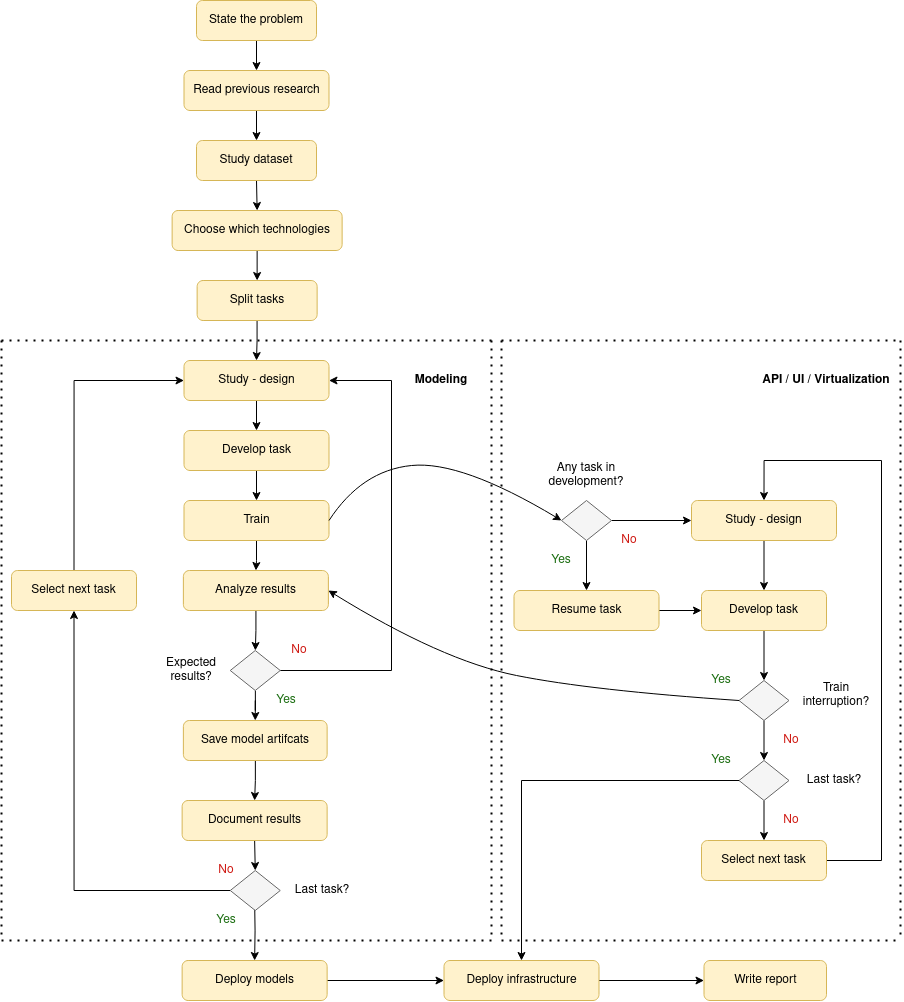
\includegraphics[width=0.82\textwidth]{imatges/planing_and_methodology/EmplyedMethodology.png}
  \caption{\textit{Development process methodology.}}
  \label{fig:flux_development}
  \end{figure}

\end{landscape}

\newpage

\section{CAD infrastructure pipeline}

Our CAD infrastructure pipeline  (see Figure \ref{fig:cad-pipeline}), consists
of different steps, beginning with data acquisition, followed by data
preprocessing. We then set up different datasets for training, validation, and
testing. Subsequently, we train the models and, assess the models gathering
metrics and finally we deploy the models under an API.

\begin{figure}[H]
  %\begin{adjustbox}{width=\textwidth, trim={0.2cm 0pt 1.5cm 0pt}, clip}
  \centering
  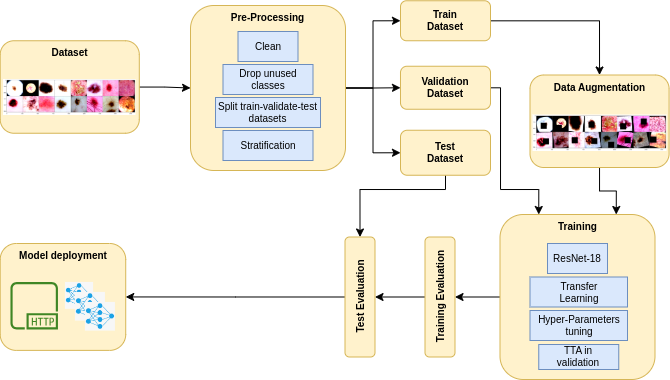
\includegraphics[width=0.9\textwidth]{imatges/methodological_contribution/Pipeline.drawio.png}
  %\end{adjustbox}
  \caption{\textit{CAD infrastructure pipeline. Train, test and deploy. }}
  {\label{fig:cad-pipeline}}
\end{figure}

\section{Data and training strategies}

Inspired by the approach of the Winning Solution to the SIIM-ISIC Melanoma
Classification Challenge \cite{WinningISIC}. The Winning Solution team observed
that in the entire dataset of 2020, comprising 33K images, only 1.76\% were
positive samples (i.e., malignant). In response, they decided to augment this
data by incorporating information from the datasets of the same competition
from the previous years (2018 and 2019). Although the individual datasets from
these earlier years were smaller, totaling 25K images, they exhibited a
positive ratio of 17.85\%. This strategic combination allowed for a more
balanced representation of positive cases in the training data. \\

To build the original dataset, we utilized 8 classes selected from the raw
dataset, as the remaining classes we considered not significant or there were
very few samples of them. Any sample that was not categorized as one of the
following classes were excluded from the training process.

\begin{itemize}
  \item melanoma
  \item nevus
  \item BCC (Basal Cell Carcinoma)
  \item BKL (Benign lesions of the keratosis)
  \item AK (Actinic Keratosis)
  \item SCC (Squamous Cell Carcinoma)
  \item VASC (Vascular Lesions)
  \item DF (Dermatofibroma)
\end{itemize}

The filtered dataset comprises 31,265 distinct image samples, demonstrating a
highly imbalanced dataset, as evident from Figure
\ref{fig:hole-dataset-distribution}.

\begin{figure}[H]
  \centering
  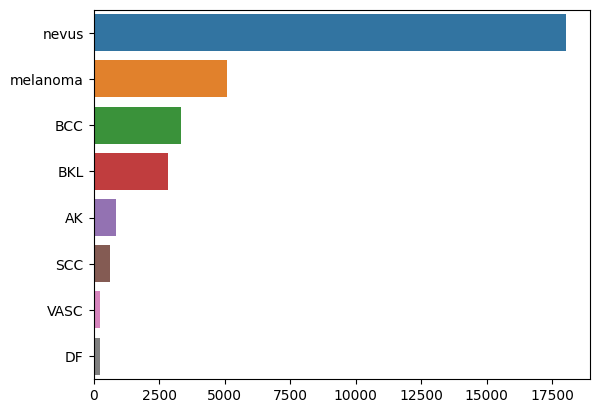
\includegraphics[width=0.75\textwidth]{imatges/data-training-strategies/hole-dataset-diagnosis.png}
  \caption[Categories distribution in dataset]{\textit{Categories distribution in dataset.}}
  {\label{fig:hole-dataset-distribution}}
\end{figure}


We started dividing the original dataset into three subsets using the Holdout
set scheme, see Figure \ref{fig:holdout-test-scheme}. \\

During the training phase, the test set remains completely separate and is not
used in any way to configure the hyper-parameters. This ensures that the
performance of a model on the test set is not artificially inflated by
adjusting hyper-parameters to achieve an exceptionally good outcome in the validation set. \\

\newpage

The data from the ISIC Archive was divided using the following percentages: 80\%
for training, 10\% for validation, and 10\% for testing. Each subset contain the same
distribution of classes as the original dataset, i.e., we applied stratification.

\begin{figure}[H]
  \centering
  \begin{adjustbox}{width=0.7\textwidth, trim={0cm 1cm 0cm 1.25cm}, clip}
    \includegraphics[width=\textwidth]{imatges/data-training-strategies/train-test-validation-sets.png}
  \end{adjustbox}
  \caption[Holdout set scheme]{\textit{Holdout set scheme. Illustration by Qualcomm}}
  {\label{fig:holdout-test-scheme}}
\end{figure}

In small to medium sized datasets, augmentation is important to prevent
overfit. For some of our trained models, we used in the training dataset our
augmentation pipelines, as illustrated in Figure \ref{fig:sample-of-datasets} and
Figure \ref{fig:aug-sample-of-datasets}, with contains the following augmentations
from the popular and powerful PyTorch augmentation library Albumentations
\cite{Albumentations}: Transpose, Flip, Rotate, RandomBrightness,
RandomContrast, MotionBlur, MedianBlur, Gaus- sianBlur, GaussNoise,
OpticalDistortion, GridDistortion, ElasticTransform, CLAHE, HueSaturationValue,
ShiftScaleRotate, Cutout.

\begin{figure}[H] \centering
  \begin{adjustbox}{width=0.9\textwidth}
    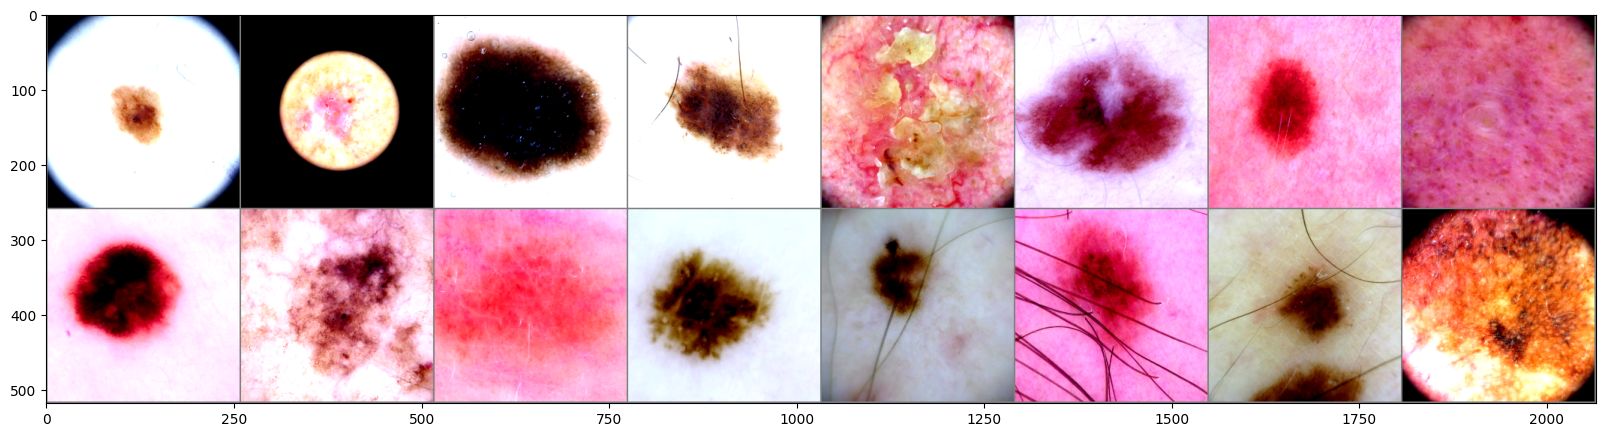
\includegraphics[width=\textwidth]{imatges/methodological_contribution/random-sample-of-isic.png}
  \end{adjustbox}
  \caption[Random sample of images]{\textit{Random sample of images.}}
  {\label{fig:sample-of-datasets}}
\end{figure}

\begin{figure}[H]
  \centering
  \begin{adjustbox}{width=0.9\textwidth}
  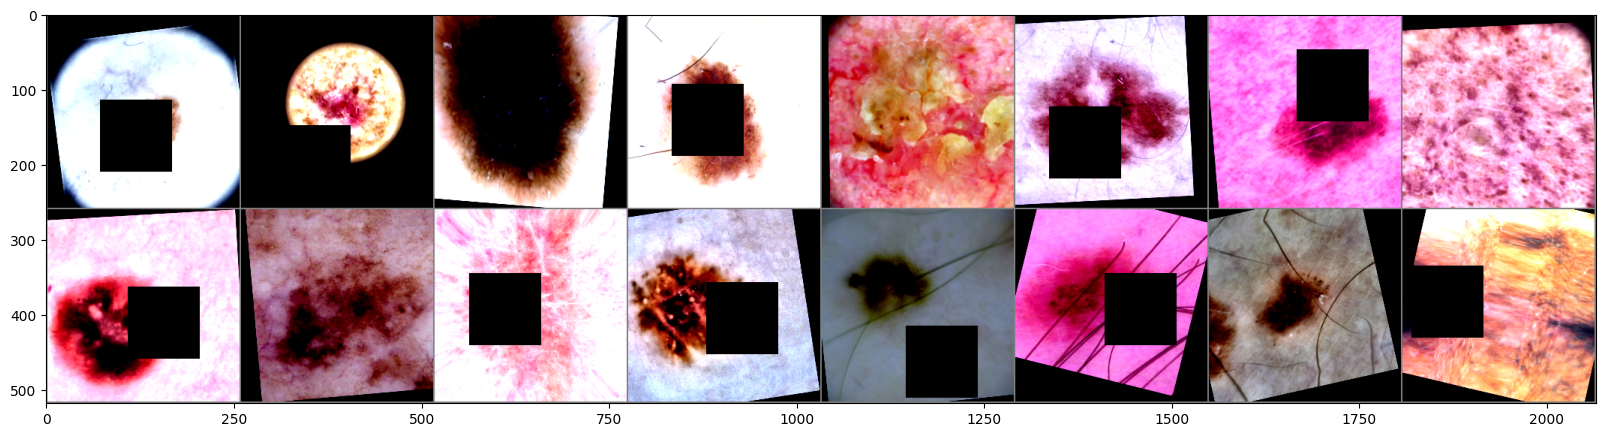
\includegraphics[width=\textwidth]{imatges/methodological_contribution/random-sample-of-isic-augmented.png}
  \end{adjustbox}
  \caption[Augmented random sample of images]{\textit{Augmented random sample of images.}}
  {\label{fig:aug-sample-of-datasets}}
\end{figure}


We decided to use as transfer model an already trained ResNet in the ImageNet
database. ResNet is short for "Residual Network," is a deep convolutional
neural network (CNN) architecture that was introduced in 2015 by researchers
from Microsoft Research \cite{ResNetPaper}. It revolutionized the field of deep
learning by addressing the challenge of training very deep neural networks. \\

There are various architectural variants or "flavors" of ResNet, including
ResNet-152,  ResNet-101,  ResNet-50,  ResNet-34, and  ResNet-18. The number
following the name of each ResNet variant indicates the number of inner layers
present in the architecture. The more the number of the layers the more the
accuracy, yet the number of parameters to be trained increase. To accurately
assess the performance of each ResNet architecture, refer to Table
\ref{table:resnet}, which provides the accuracy achieved on the ImageNet
dataset along with the corresponding number of trainable parameters in
millions.

\begin{table}[H]
  \centering
  \begin{tabular}{lcc}
    \toprule
    \textbf{Model} & \textbf{Accuracy} & \textbf{Parameters} \\
    \midrule
    ResNet-152 & 78.31\% & 60.2M \\
    ResNet-101 & 77.37\% & 44.5M \\
    ResNet-50 & 76.15\% & 25.6M \\
    ResNet-34 & 73.30\% & 21.8M \\
    ResNet-18 & 69.76\% & 11.7M \\
    \bottomrule
  \end{tabular}
  \caption[Accuracy achieved on ImageNet and trainable parameters of each ResNet]
  {\textit{Accuracy achieved on ImageNet and trainable parameters of each ResNet.
  Each image in the ImageNet dataset is associated with 1 of 1,000 classes. Table by paperswithcode}}
  {\label{table:resnet}}
\end{table}

We decided to use ResNet18 as base model only for technical reasons and time
constrains. The lack of powerfull GPUs took us to pick this estimator agains
the others. There are other architectures that we could have tried as: AlexNet,
ResNetXt, VGG, etc, but comparing the performance of those models in the
SIIM-ISIC Melanoma competition is not the goal of this thesis.

\section{Validation strategy}

In any machine learning project, it is critical to establish a reliable
validation scheme to properly evaluate and compare models. This becomes
particularly crucial when dealing with a small to medium-sized dataset or when
the evaluation metric is unstable, as is the case with the dataset provided in
the competition. There are various metrics commonly used to assess the quality of a model's
predictions. We present a selection of metrics that we find relevant for
evaluating our models. \\

A confusion matrix (see Figure \ref{fig:confusion-matrix}) is a square matrix
with dimensions {\tt NxN}, where {\tt N} represents the total number of classes being
predicted.

\begin{figure}[H]
  \begin{adjustbox}{trim={0pt 0.5cm 0pt 1cm}, clip}
    \centering
    \includegraphics[width=0.9\textwidth]{imatges/validation-strategy/confusion-matrix.png}
  \end{adjustbox}
  \caption[Confusion matrix multi-class]{\textit{Confusion matrix multi-class. Illustration by kaggle}}
  {\label{fig:confusion-matrix}}
\end{figure}

From confusion matrix we can obtain other metrics such as:

\begin{itemize}

  \item {\bf Accuracy}

    The Accuracy metric, calculates the ratio of correct predictions to the total number of
    predictions made on a dataset. It is not a good matric when working with
    unbalanced datasets.

    \[Accuracy = \frac{TP + TN}{TP + TN + FP + FN}\]

  \item {\bf True Positive Rate (TPR) or Sensitivity}

    The True Positive Rate tells about how many of the true class samples were
    correctly classified.

    \[TPR = \frac{TP}{TP + FN}\]


  \item {\bf False Positive Rate (FPR) or False Alarm Ratio}

    The False Positive Rate tells the proportion of the true class samples that
    were not correctly classified and are False Positive.

    \[FPR = \frac{FP}{FP + TN}\]


  \item {\bf Receiver Operator Characteristic (ROC)}

	  An ROC curve plots TPR vs. FPR at different classification thresholds {\tt
	  T}, where $T \ \text{for} \ 0 <= x <= 1$. Lowering the classification
	  threshold classifies more items as positive, thus increasing both False
	  Positives and True Positives. By plotting the curve, you can say which
	  threshold is better, depeding on how many False Positive we are willing to
	  accept.

    \begin{figure}[H]
      \centering
      \begin{adjustbox}{trim={0pt 0cm 0pt 0cm}, clip}
        \centering
        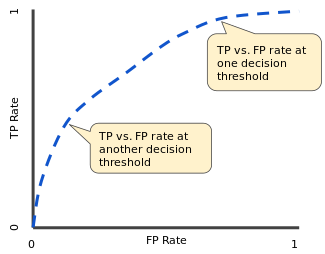
\includegraphics[width=0.55\textwidth]{imatges/validation-strategy/ROCCurve.png}
      \end{adjustbox}
        \caption{\textit{Typical ROC Curve. Illustration by Alphabet Inc.}}
      {\label{fig:ROCCurve}}
    \end{figure}


  \item {\bf Area Under the Curve (AUC)}

  The Area Under the Curve is a value between 0 and 1 that measures the
  ability of a classifier to distinguish between classes. It is used as a summary of
  the ROC curve. The higher the AUC, the better the performance of the model at
  distinguishing between the positive and negative classes.

  \begin{figure}[H]
    \centering
    \includegraphics[width=0.7\textwidth]{imatges/validation-strategy/auc.png}
    \caption[AUC-ROC performance]{\textit{AUC comparation. Illustration by Elizabeth Louise Thomas}}
    {\label{fig:auc-roc}}
  \end{figure}

\end{itemize}

\newpage

\section{Models metrics}

The training phase ended with the development of eight models using an
imbalanced dataset comprising eight classes. Various learning policies and
Artificial Intelligence (AI) techniques were tested during the experimentation
process.

These models were divided into two categories: one without any
additional regularization and another with additional regularization techniques
such as data augmentation and the inclusion of dropout layers.

\begin{table}[H]
\centering
\begin{tabular}{lc|lc}
    \toprule
  \textbf{Model} & \textbf{Test AUC} & \cellcolor{gray!50}\textbf{Model} & \cellcolor{gray!50}\textbf{Test AUC}  \\
\midrule
 M0 & 0.892 & \cellcolor{gray!50}M4 & \cellcolor{gray!50}0.858 \\
 M1 $\star$ & 0.892 & \cellcolor{gray!50}M5 $\star$ & \cellcolor{gray!50}0.843 \\
 M2 $\ast$ &  0.885 &  \cellcolor{gray!50}M6 $\ast$ & \cellcolor{gray!50}0.848 \\
 M3 $\bullet$ & 0.886 & \cellcolor{gray!50}M7 $\bullet$ & \cellcolor{gray!50}0.849 \\
 \midrule
Mean &  88.875\% & \cellcolor{gray!50}Mean & \cellcolor{gray!50}84.950\%  \\
SD &  0.377\%  &   \cellcolor{gray!50}SD &  \cellcolor{gray!50}0.625\%  \\

\bottomrule
\end{tabular}
\caption[Models metrics in test dataset]
  {\textit{Models metrics in test dataset.}}
{\label{table:test-set-resume-metrics}}
\end{table}

The initial group of models performed well on the test set with an average AUC
of 88.875\% and a small standard deviation of ±0.377\%. However, they showed
signs of overfitting on the validation set. In contrast, the second group of
models, trained with additional regularization techniques, achieved lower
results but did not suffer from overfitting. They had an average AUC of 84.950%
with a standard deviation of ±0.625\%, which was influenced by more training
epochs.

During model training, we also developed the necessary CAD infrastructure. For
the API, we used a flexible approach with soft configurations that could be
specified through file-based parameters, offering adaptability and simplified
management. Additionally, we created an intuitive UI for seamless interaction
between healthcare professionals and the models.

We also provided a Docker-based script for easy deployment of the
infrastructure on any Linux operating system, ensuring efficient startup and
operation.

\section{CAD infrastructure result}


\chapter*{Gratitudes}
%\label{cap:agraiments}

Per començar vull agrair molt especialment a \ldots


\tableofcontents

\listoffigures

\listoftables

\mainmatter

\chapter{Introduction}
\label{cap:intro}

\section{Problem Statement}

Skin cancer, including melanoma, represents a significant public health concern worldwide. Melanoma, in particular, poses a considerable challenge due to its high mortality rate and the need for early detection for successful treatment. Early and correct diagnosis is key for ensuring patients have the best possible prognosis.
Melanoma misdiagnosis accounts for more pathology and dermatology malpractice claims than any
cancer other than breast cancer, as an early misdiagnosis can significantly reduce a patient’s chances of
survival \cite{Melanoma}. \\

Dermoscopy, also known as dermatoscopy \textit{Figure \ref{fig:procedure_dermoscopy}}, is a noninvasive technique widely utilized for the examination of cutaneous lesions. It involves the use of a handheld instrument called a dermatoscope to visualize subsurface skin structures that are typically not visible to the naked eye. The dermatoscope illuminates the skin surface and provides magnification, allowing for a detailed examination of the epidermis, the dermoepidermal junction, and the papillary dermis. By analyzing these structures, dermatologists can identify specific features and patterns associated with various skin conditions, including melanoma \cite{Dermoscopy}.

\begin{figure}[htb]
\centering

\includegraphics[width=6.5 cm]{imatges/introduction/medical_procedure_dermastocopy.jpeg}
\caption[Dermoscopy Procedure]{\textit{During the dermoscopy procedure, the dermatologist places the dermatoscope directly on the skin, making contact with the lesion of interest. Illustration by MD Anderson Cancer Center}}
{\label{fig:procedure_dermoscopy}}
\end{figure}

Worldwide, in 2020 an estimated 324,635 people were diagnosed with melanoma and an estimated 57,043 people worldwide died from melanoma the same year \cite{CancerStats}. The introduction of sophisticated machinery and techniques in dermoscopy procedures \textit{Figure \ref{fig:subset_isic}} seems not enough to fight against melanoma, but the developments in artificial intelligence (AI) especially in deep learning techniques, have made Computer-Aided Diagnosis (CAD)\footnote{Computer-Aided Diagnosis (CAD) refers to the use of computer algorithms and technologies to assist healthcare professionals in the process of medical diagnosis} a promising path towards medical automation.

\begin{figure}[h!]
\centering
\begin{subfigure}{0.3\textwidth}
    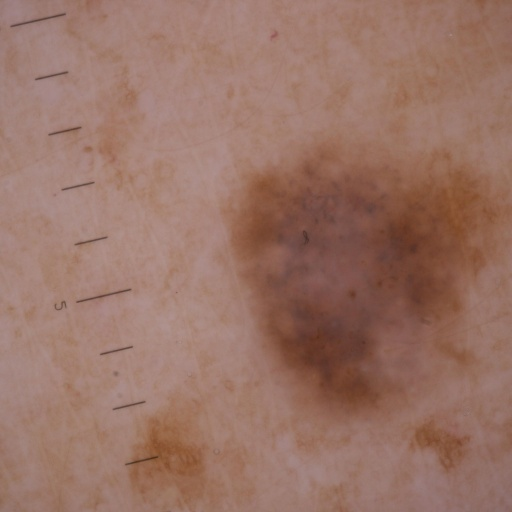
\includegraphics[width=\textwidth]{imatges/introduction/subset_isic/ISIC_1752943.jpg}
\end{subfigure}
\hfill
\begin{subfigure}{0.3\textwidth}
    
\includegraphics[width=\textwidth]{imatges/introduction/subset_isic/ISIC_1766619.jpg}
\end{subfigure}
\hfill
\begin{subfigure}{0.3\textwidth}
    
\includegraphics[width=\textwidth]{imatges/introduction/subset_isic/ISIC_1448526.jpg}
\end{subfigure}
\caption[Dermoscopy Images]{\textit{Dermoscopy Images. Illustration by ISIC Archive}}
\label{fig:subset_isic}
\end{figure}

However, there are several limitations that raise doubts about the effectiveness of automated melanoma cancer classifiers and their suitability for integration into the medical system. Firstly, certain methods are constructed based on theoretical models of melanoma appearance, which may restrict their applicability to specific morphologies and fail to capture the wide range of variations seen in real-world scenarios. Secondly, AI systems utilized in these classifiers are trained to address a singular and narrow task. Unlike human dermatologists, these systems lack the ability to consider holistic patient information when formulating a final diagnosis, reflecting the concept of weak AI \cite{WeakAI}. Lastly, numerous methods have been trained and evaluated using high-quality image frames, which may result in instability when applied under real-time visibility conditions where image quality is often compromised. A fundamental part of machine learning is the problem of generalization, that
is, how to make sure that a trained model performs well on unseen data. If the
unseen data has different distribution, i.e. a domain shift exists, the problem is
significantly more difficult even the smallest changes in the statistics
as compared to the training data can cause a deep neural network to fail completely \cite{DomainShift}. \\

Addressing these limitations and developing melanoma cancer classifiers that encompass a wider range of morphologies, incorporate holistic patient information, consider relevant elements, and demonstrate robustness in real-world scenarios are crucial for improving the reliability and effectiveness of melanoma detection and diagnosis systems. \\

\section{Project Objectives}

The main objective of this project is to create a health care infrastructure, focused on melanoma detection using deep learning methods to train
a system capable of detecting melanoma on dermoscopy images to test the ability
of computer-assisted image analysis. To this end, the gradual achievements
that must be accomplished are:

\begin{itemize}
    \item Gaining a comprehensive understanding of the theory behind deep learning and its practical applications.
    \item Analyzing images from dermostocopy and understanding its most important features.
    \item Train deep learning models with different techniques based on tranfer-learning focused on the images of the melanoma ISIC Challenge \cite{IsicChallenge}.
    \item Developing a CAD system. The CAD system contains the already trained models with a simple web UI\footnote{The user interface (UI) is the point of human-computer interaction and communication in a device} an API\footnote{API stands for Application Programming Interface} and finally a mechanism using Docker to virtualize this services making it ease to deploy in any based Linux System.
\end{itemize}

\section{Personal Motivation}

I envisioned this project as a unique fusion of three personal passions. Firstly, I was fueled by a deep fascination with human cognition and reasoning. Machines, in my eyes, represented a novel paradigm through which I could delve further into this captivating realm. \\

I am also motivated by the remarkable problem-solving capacity of data. Regardless of its structure, data holds immense potential to uncover hidden patterns, provide insights, and drive innovation. The ability to extract meaningful information from data, regardless of its form, inspires me to constantly expand my knowledge and skills in order to contribute to the field of data science and make a tangible difference in the world. \\

Last but not least, I am driven by the immense power of automation and its ability to democratize access to research knowledge. I am amazed by how automation processes can extract value and make them readily available to professionals and the public alike.

\section{Statement of Originality}

I, Wilber Eduardo Bermeo Quito, declare that the thesis titled "A platform for classifying melanoma" is an original work completed with the support and collaboration of Accenture SL and the VICOROB laboratory. \\

The content presented in this thesis is the outcome of my independent research efforts, guided by the knowledge and expertise acquired through my academic studies and the valuable contributions from Accenture S.L and the VICOROB laboratory. \\

I acknowledge the importance of academic integrity and the consequences of plagiarism. Hence, I affirm that all the information, data, results, figures, and conclusions presented in this thesis are authentic and original. Any references or sources used have been appropriately cited and referenced.

\section{Regulatory Framework}

The inclusion of legal considerations has become a significant aspect of the field of medical imaging. Privacy concerns and the potential misuse of personal information make sharing and distributing medical data particularly challenging. To address these limitations, recent research collaborations have focused on promoting the sharing of patient data through de-identification methods. However, it is crucial to thoroughly analyze the obligations related to the protection of individuals and their personal data before engaging in projects involving medical imaging. \\

When working with medical images, it is the utmost importance to prioritize patient privacy rights. In the context of developing a skin lesions database, it is necessary to obtain signed consent from patients for the publication of their data. For this thesis, the ISIC Archive database was utilized, this database serves as a publicly accessible resource for teaching, research, and the development and testing of diagnostic artificial intelligence algorithms, and it resolves any concerns related to consent \cite{IsicArchive}. It is a large and continually expanding open-source archive of skin images.

\section{Related Work}

Melanoma Computer-Aided Diagnosis (CAD) classifiers have been a subject of extensive research and development in recent years,
also there has been a lot of work in platforms capable of explaining the way these models infer.
Bellow is mentioned remarkable related work to the subject. \\

\vspace{0.5cm}
\textbf{Identifying Melanoma Images using EfficientNet Ensemble: Winning Solution to the SIIM-ISIC Melanoma Classification Challenge} \\

Winning solution to the SIIM-ISIC Melanoma Classification Challenge. It is an ensemble of convolutions of neural network (CNN) models with different backbones and input sizes \cite{WinningISIC}.  \\

\vspace{0.5cm}
\textbf{Dermatologist-level classification of skin cancer with deep neural networks} \\

This study demonstrated the use of a deep learning algorithm to classify skin lesions, including melanoma, with accuracy comparable to dermatologists. The deep neural network was trained on a large dataset of images and achieved high sensitivity and specificity \cite{SkinCancerDeepNN}. \\

\vspace{0.5cm}
\textbf{Computerized analysis of pigmented skin lesions: A review}  \\

The goal of this paper is to give a detailed explanation and clear up any confusion about the words and phrases used in melanoma studies. And to organize and group together useful sources, making it easier to find information on a particular sub-topic when searching through the existing literature \cite{MelanomaTopicsReview}. \\

\newpage

\vspace{0.5cm}
\textbf{CNN-Explainer} \\

The CNN-Explainer is an interactive web-based tool that aims to provide explanations for the predictions made by convolutional neural network (CNN) models \cite{CNNExplainer}.

\section{Contribution to Melanoma Detection}

In this section, we present the contribution to the field of melanoma detection through the development of a melanoma CAD (Computer-Aided Diagnosis) infrastructure classifier. \\

The thesis comprises multiple models employing various techniques, including transfer learning, data augmentation, just-in-time testing, regularization, and others. To compare these models, tools like W\&B (Weight \& Biases), a MLOps platform for experiment tracking, and MLXTEND, providing utilities and extensions for machine learning and data science in Python's scientific computing stack, were utilized. The experiments were conducted using the ISIC Archive dataset, consisting of benign and malignant skin lesions. Prior to analysis, the dataset underwent preprocessing to enhance quality and normalize features. Consequently, accurate classification and differentiation of melanoma lesions from benign ones were achieved. \\

In order to improve the distribution and usability of all models, two services were developed. These services include a user-friendly UI and an API, both of which were containerized using Docker technology. By containerizing the UI, an intuitive and interactive user experience was provided, enabling users to seamlessly interact with the melanoma CAD system. Similarly, containerizing the API streamlined request handling and prediction serving, resulting in efficient performance. This approach facilitated easy deployment across various platforms.


\chapter{State of the Art}
\label{cap:estat}

Melanoma, a type of cancer that arises from melanin-producing cells,
can be found in various parts of the body such as the skin, eyes, nerve centers, and meninges. Early diagnosis is crucial for improving the chances of curing melanoma, even though it has the highest increasing incidence rate among all skin cancer types.
According to a study \cite{TimelyMelanomaDetection}, timely identification of early-stage skin cancer resulted in a significant 90\%
reduction in mortality rates. For instance, patients diagnosed with stage I melanoma have a 10-year overall survival
probability ranging from 94\% to 98\%, while those in stage IV have a much lower estimated 10-year
overall survival rate of just 10\% to 15\%. \\

Dermoscopy is a non-surgical method used to examine the underlying layers of the skin.
While it can yield good results, it requires extensive training and experience in dermatology.
However, it may not provide a definitive diagnosis for melanoma, especially in its early stages.
Consequently, there is a need for an automated diagnostic tool. \\

In a study \cite{EpidemiologySkinCancer} the melanoma task classification was compared between expert
opinions and artificial neural networks.
The computer program demonstrated had an area under the receiver
operating characteristic curve of 0.87, which was higher than the dermatologists (0.74), the program also
had a higher sensitivity in classification of 85\% against the 76\% by the dermatologists.
These findings indicate the potential utilization of automated systems in the field of cancer detection. \\

For cancer prediction, a mostly supervised learning approach is employed that makes use of algorithms for classification based on conditional decisions or probabilities. The most common algorithms or methodologies include decision trees, convolutional neural networks (CNN), support vector machine (SVM), and k-nearest neighbors (KNN). One of the most powerful systems are CNNs (Convolutional Neural Networks), despite the fact that their use may involve a loss of explainability, which is a major concern in healthcare systems. \\

Although this project goes beyond the mere creation of highly accurate models for classifying Melanoma, I have taken into consideration and reviewed related works that have influenced and guided my own path.

\section{Identifying Melanoma Images Using EfficientNet Ensemble}

This is the winning approach to the SIIM-ISIC Melanoma Classification Challenge \cite{ISICKaggle}. The team not only let the competition source code available on GitHub \cite{WinningISICGithub} but they also wrote a paper explaining in detail their investigation \cite{WinningISIC}. \\

The project is an ensemble of convolutional neural network (CNN) models. These models utilize different backbones and input sizes, primarily focusing on image data, although some also incorporate image-level and patient-level metadata. The success of the project can be attributed to several factors:

\begin{itemize}
    \item Implementation of a stable validation scheme.
    \item Effective selection of the model target.
    \item Thoughtful optimization of the pipeline.
    \item Utilization of ensemble learning with highly diverse models.
\end{itemize}

The submission that won achieved an AUC (Area Under the Curve)\footnote{AUC is a metric that quantifies the overall quality of a binary classification model by measuring the area under its ROC curve. It provides a single value that summarizes the model's ability to discriminate between positive and negative instances.} score of 0.9600 on cross-validation and 0.9490 on the private leaderboard. \\

From their work, I adopted various deep learning techniques. For instance, I learned about evaluating models on unbalanced multi-class data-sets like the ISIC dataset. To properly assess the training process, they utilized the AUC with one-vs-rest (OvR) metric. This project as well uses this metric to to evaluate the performance of the models. \\

Additionally, this thesis incorporated an early-stop mechanism into the training process. This mechanism prevents over-fitting by monitoring the model's performance on a validation set and stopping the training if the performance starts to worsen or stagnate. This was not mentioned in the related work, but I recognized its importance and included it in my implementation. \\

Another aspect the current thesis borrowed from this work is the approach to cleaning and mapping data-sets from different years. They trained their models with different output sizes, but the process of mapping and joining the data-sets into a single data-set was similar to my approach, where I consistently mapped the data into eight different classes. \\

The pipeline of data augmentation that is implemented in the work is also reused. As they do, this thessis use Albumentations\cite{Albumentations} library instead of the native alternative transforms data agumentation from Pytorch. \\

These inspirations and adaptations from the related work have greatly influenced the development and organization of this deep learning project.

\section{CNN Explainer}

CNN explainer is a web page created through a collaborative research effort between Georgia Tech and Oregon State\cite{CNNExplainer}. It leverages TensorFlow.js, a deep learning library that utilizes GPU acceleration within the web browser, to load pretrained models for visualization. The entire interactive system is implemented in JavaScript, utilizing Svelte as a framework and D3.js for visualizations. With CNN Explainer, users can upload images and obtain predictions for those images across ten different classes. \\

While CNN Explainer primarily aims to serve educational purposes, my project's UI focuses on providing dermoscopy images predictions and information about the models used and their outputs. The inspiration for incorporating an interactive UI for end users stemmed from CNN Explainer. Consequently, I utilized the same web framework to develop the UI for my project.


\chapter{Domain}
\label{cap:problem_domain}

In this chapter, we will delve into the details of melanoma cancer, its origins, reasons for its development, and strategies to minimize the risk of its occurrence. We will also explore other common types of skin cancer and their underlying causes. By the end, I hope you have a bigger view and understanding of these conditions and be equipped with knowledge. \\

\section{The Skin}

The skin, our body's largest organ \cite{BaseCancerKnowledge}, plays a vital role in protecting us from external threats and maintaining our overall well-being. Let's explore the three main layers of the skin in more detail:

\begin{itemize}
 \item \textbf{Epidermis} \\
 
The epidermis is the outermost layer of the skin, serving as a protective shield against environmental factors. It consists mainly of flat, scale-like cells called keratinocytes. These cells produce a tough protein called keratin, which helps make the skin waterproof and resistant to damage. Within the epidermis, specialized cells called melanocytes produce melanin, the pigment responsible for skin color. Melanin also helps protect the skin from harmful ultraviolet (UV) radiation. \\

The epidermis is made up of several layers, including the stratum corneum, the topmost layer composed of dead skin cells that are continuously shed and replaced by new cells from the lower layers. The epidermis also contains other types of cells, such as Langerhans cells, which are part of the immune system and help defend against infections.

\item \textbf{Dermis} \\

Beneath the epidermis lies the dermis, a complex layer that provides structural support to the skin. The dermis contains a network of blood vessels that supply nutrients and oxygen to the skin cells. It also houses various structures, including hair follicles, sweat glands, sebaceous glands, and nerve endings.
The dermis is composed of collagen and elastin fibers, which give the skin its strength, elasticity, and flexibility. These fibers allow the skin to stretch and recoil as needed. The dermis also plays a crucial role in thermoregulation by regulating blood flow to control body temperature.

\item \textbf{Hypodermis (Subcutaneous Tissue)} \\

The deepest layer of the skin is called the hypodermis or subcutaneous tissue. It is primarily made up of adipose tissue, which provides insulation, cushioning, and energy storage. The hypodermis helps to regulate body temperature by acting as an insulating layer, preventing heat loss. It also acts as a shock absorber, protecting the underlying structures and organs from injury.
Additionally, the hypodermis serves as a connection between the skin and the underlying muscles and bones. It contains blood vessels and nerve endings that supply nutrients and sensation to the skin.

\end{itemize}

In order to visualize the structure of the skin and understand the dimensions of each layer, \textit{Figure \ref{fig:melanoma_diagram}} provides a representation of the three main layers of the skin: the epidermis, dermis, and hypodermis.

\begin{figure}[H]
\centering
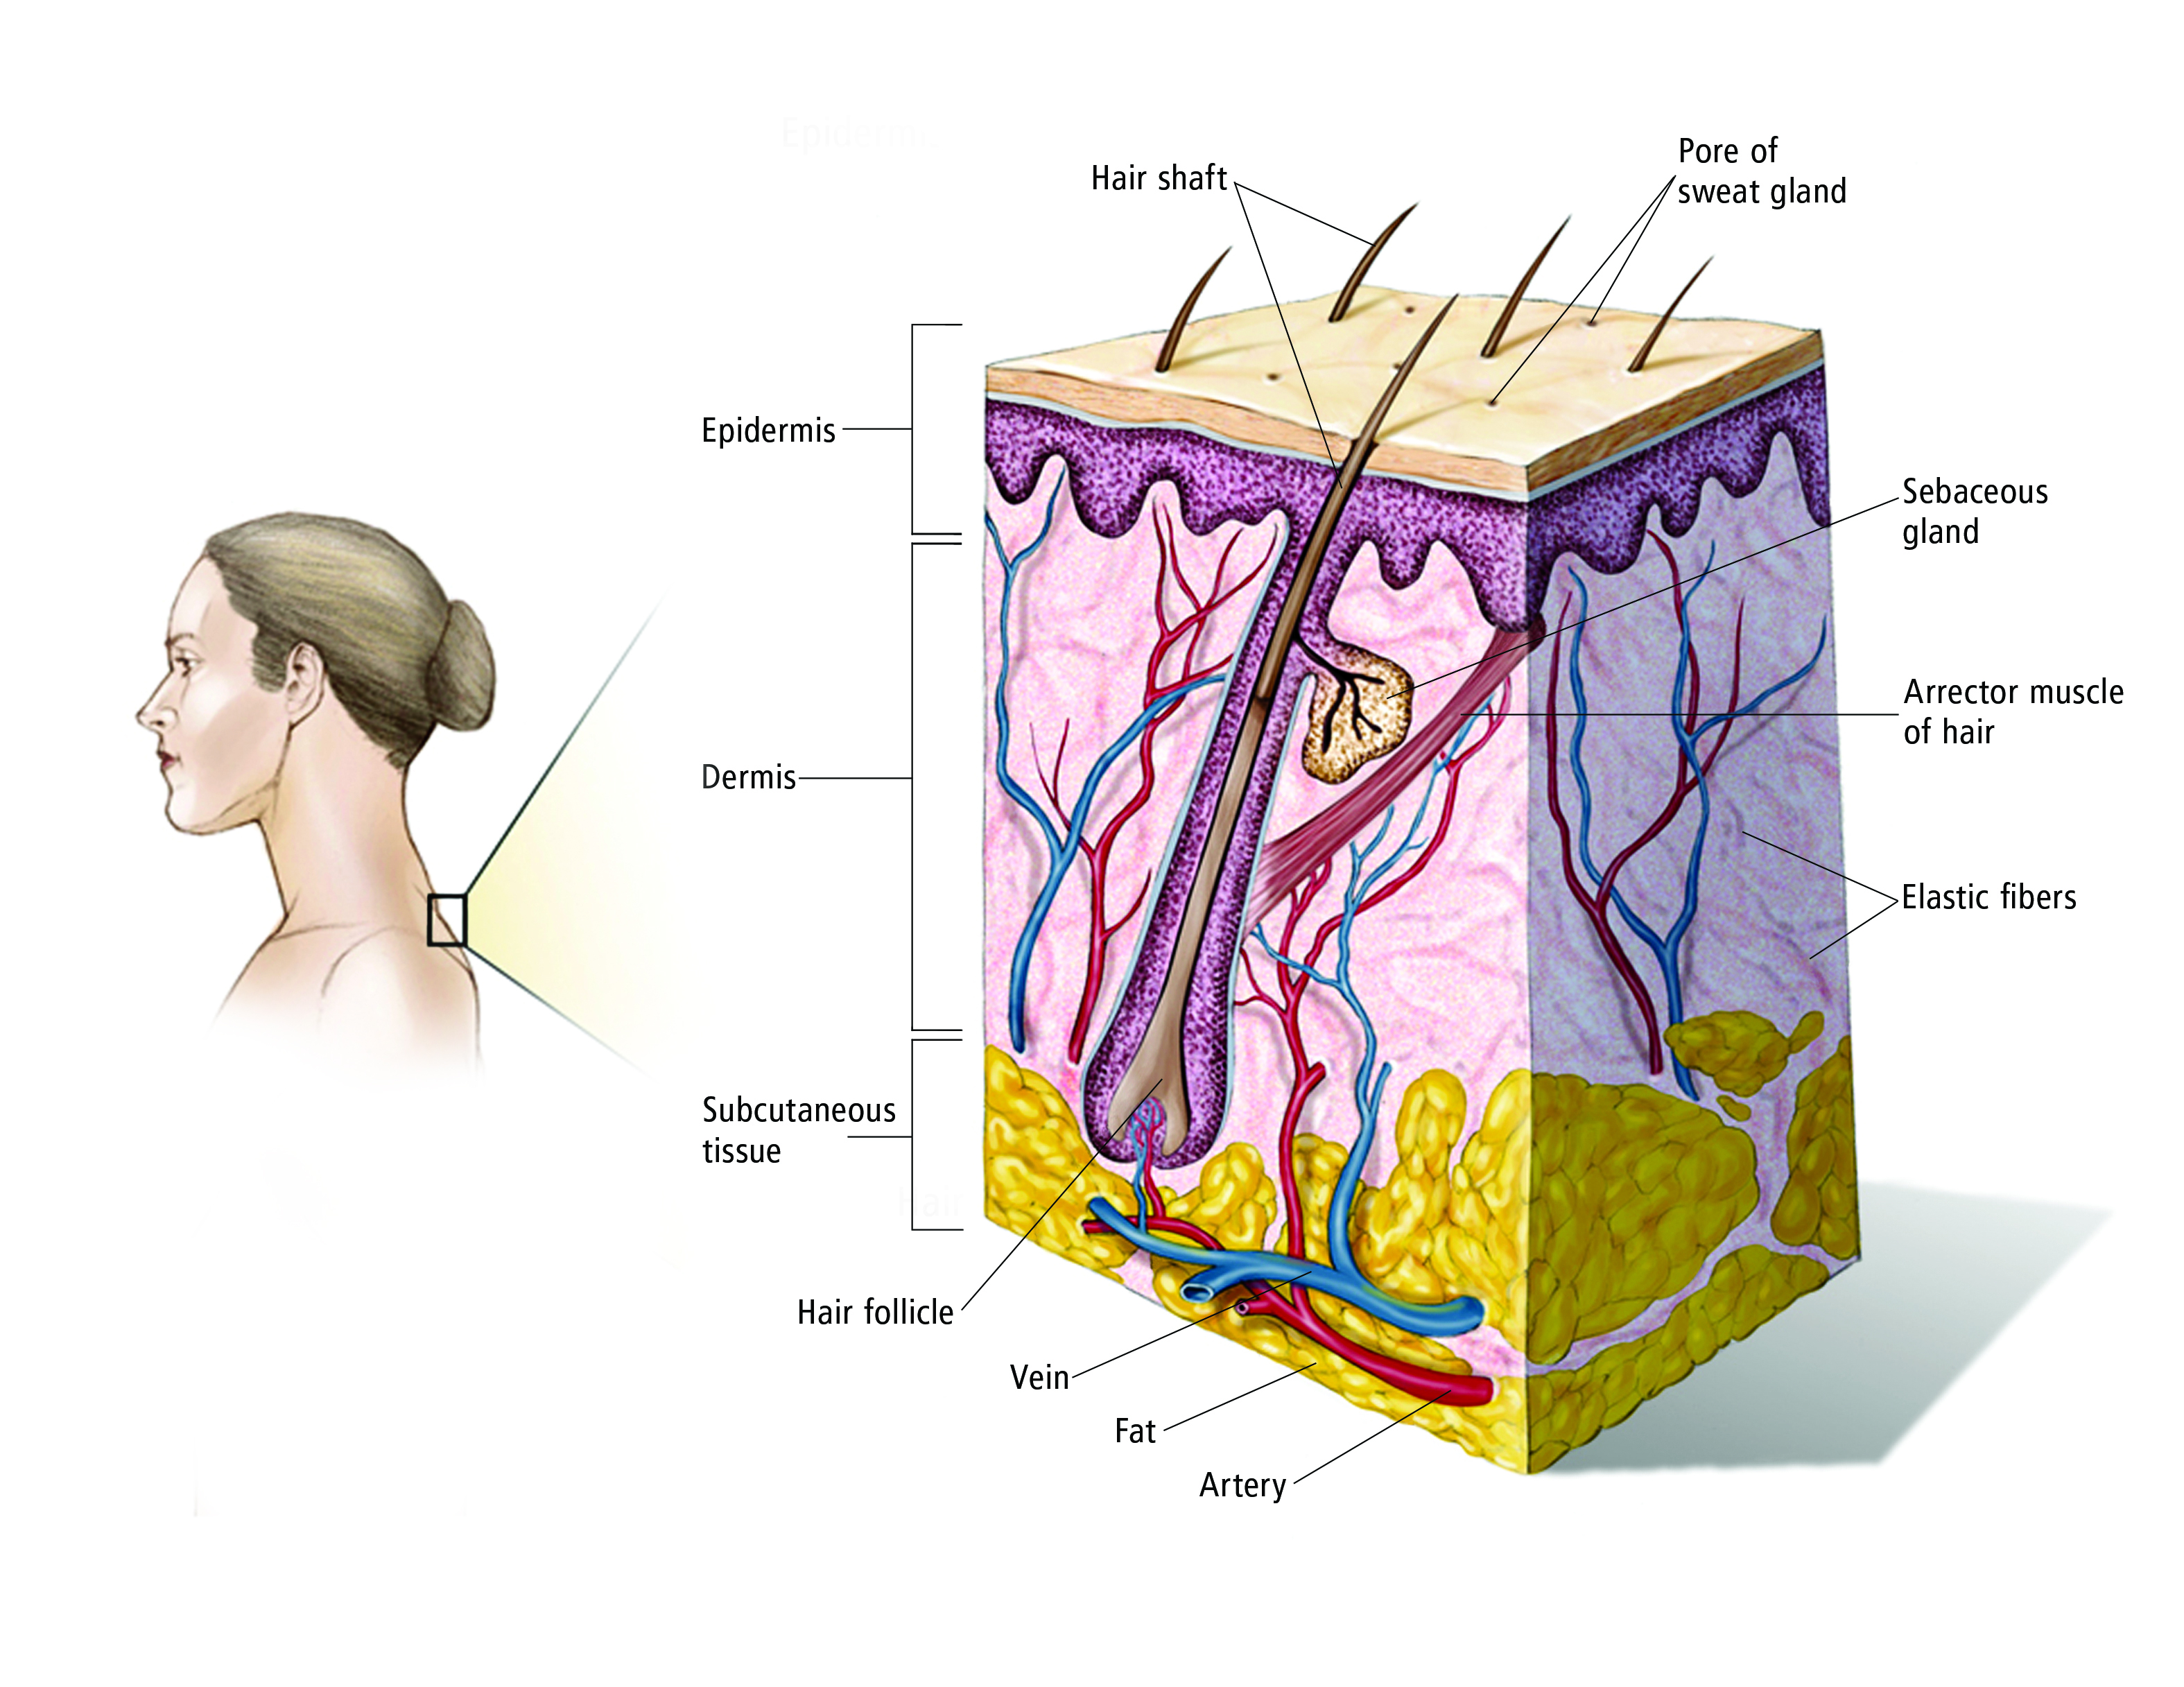
\includegraphics[width=0.85\textwidth]{imatges/problem_domain/melanoma-diagram.jpg}
\caption[Skin Main Layers]{\textit{Skin Main Layers. Illustration by Cancer.Net}}
{\label{fig:melanoma_diagram}}
\end{figure}

\section{Skin Cancer}

Cancer begins when healthy cells undergo changes that cause them to grow and divide uncontrollably, forming a mass known as a tumor. Tumors can be classified as either cancerous or benign. A cancerous tumor is considered malignant, meaning it has the potential to invade nearby tissues and spread to other parts of the body through a process called metastasis. Conversely, a benign tumor may grow locally but does not have the ability to spread to other areas. \\

Skin cancer is one of the most prevalent types of cancer, with over 3 million Americans diagnosed each year. However, the prognosis for skin cancer is generally favorable when detected early. Treatment options for skin cancer often involve topical medications, in-office procedures performed by dermatologists, or outpatient surgeries. Dermatologists specialize in diagnosing and treating conditions of the skin. As a result, skin cancer accounts for less than 1\% of all cancer-related deaths. \\

In more advanced cases, skin cancer may require comprehensive medical care provided by a multidisciplinary team, which typically includes a dermatologist, surgical oncologist, radiation oncologist, and clinical oncologist.

\subsection{Types of Skin Cancer}

There are three primary forms of skin cancer \cite{BaseCancerKnowledge}. \\

\vspace{0.5cm}
\textbf{Basal cell carcinoma} \\

This skin cancer arises from basal cells located in the lower epidermis. Approximately 80\% to 90\% of skin cancers originate from these cells, leading to the designation of basal cell carcinomas. They typically develop on the head and neck, although they can occur anywhere on the skin. Sun exposure is the primary cause, although they may also occur in individuals who underwent radiation therapy during childhood. This type of skin cancer generally grows slowly and rarely metastasizes to other parts of the body. \\

\vspace{0.5cm}
\textbf{Squamous cell carcinoma} \\

This skin cancer originates from flat, scale-like cells known as squamous cells that comprise a significant portion of the epidermis. Around 10\% to 20\% of skin cancers develop from these cells, resulting in the classification of squamous cell carcinomas. Sun exposure is the main cause, and they can be diagnosed on various regions of the skin. They may also emerge on skin that has been burned, damaged by chemicals, or exposed to x-rays. Common sites for squamous cell carcinoma include the lips, areas with long-standing scars, and the skin surrounding the mouth, anus, and vagina. Roughly 2\% to 5\% of squamous cell carcinomas metastasize to other parts of the body. \\

\vspace{0.5cm}
\textbf{Melanoma} \\

The most aggressive type of skin cancer, originates in scattered cells known as melanocytes where the epidermis and dermis meet. Melanocytes produce the pigment melanin, responsible for skin color. Melanoma accounts for approximately 1\% of all skin cancers. 

\newpage

\subsection{Stages of Skin Cancer}

The following stages are used for basal cell carcinoma. Basal cell carcinoma accounts for more than 90\% of all skin cancers in the United States and is the most common of all cancers. Typically, it is a slow-growing cancer that seldom spreads to other parts of the body \cite{CancerInstitute}. \\

\textbf{Stage I} \\

In stage I, abnormal cells are found in the squamous cell or basal cell layer of the epidermis. These abnormal cells may become cancer and spread into nearby normal tissue. 

\begin{figure}[H]
\centering
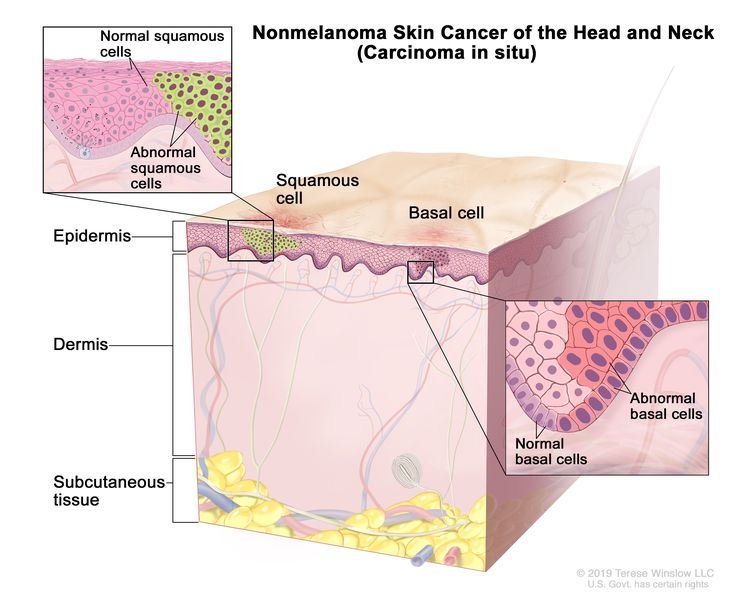
\includegraphics[width=0.7\textwidth]{imatges/problem_domain/phase0-skin-cancer.jpg}
\caption[Skin Cancer, Stage I]{\textit{Skin Cancer, Stage I. Abnormal cells are found in the squamous cell or basal cell layer of the epidermis. These abnormal cells may become cancer and spread into nearby normal tissue. Illustration by Terese Winslow}}
{\label{fig:stage0-skin-canceer}}
\end{figure}

\textbf{Stage II} \\

In stage II, cancer has formed and the tumor is 2 centimeters or smaller. 

\begin{figure}[H]
\centering
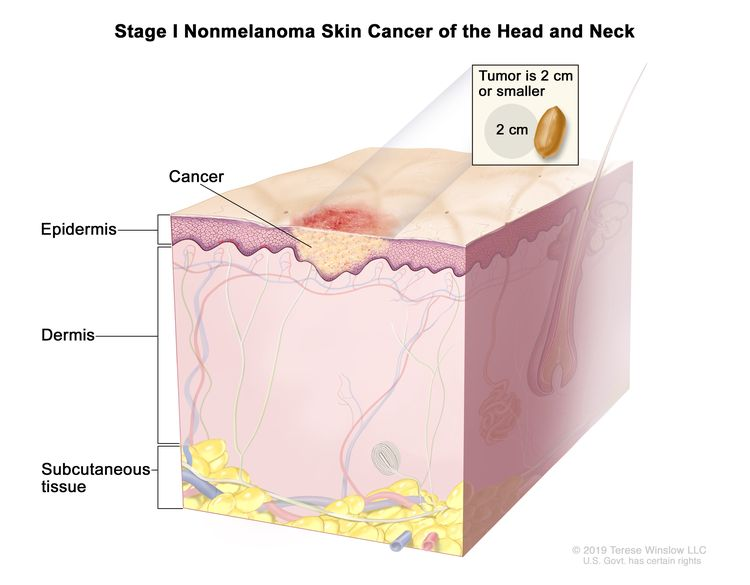
\includegraphics[width=0.7\textwidth]{imatges/problem_domain/stage1-skin-cancer.jpg}
\caption[Skin Cancer, Stage II]{\textit{Skin Cancer, Stage II. In stage II, cancer has formed and the tumor is 2 centimeters or smaller. Illustration by Terese Winslow}}
{\label{fig:stage1-skin-canceer}}
\end{figure}

\textbf{Stage III} \\

In stage II, the tumor is larger than 2 centimeters but not larger than 4 centimeters.

\begin{figure}[H]
\centering
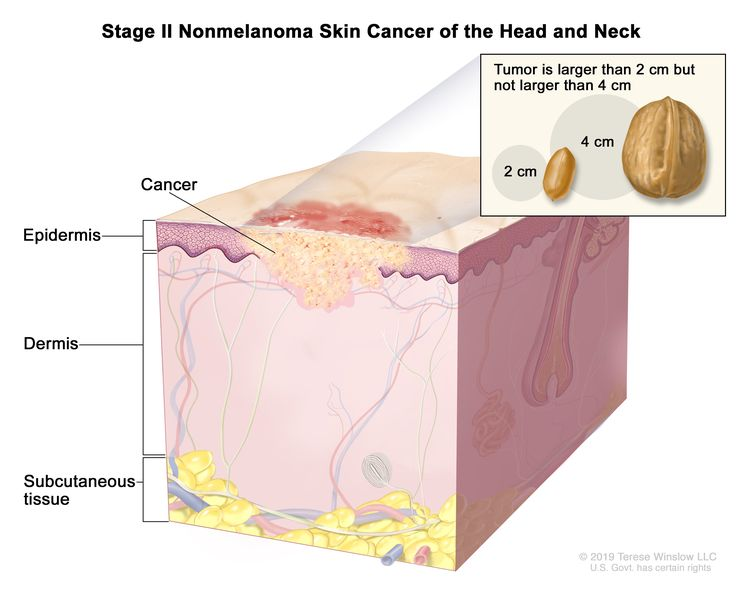
\includegraphics[width=0.7\textwidth]{imatges/problem_domain/stage2-skin-cancer.jpg}
\caption[Skin Cancer, Stage III]{\textit{Skin Cancer, Stage III. The tumor is larger than 2 centimeters but not larger than 4 centimeters. Illustration by Terese Winslow}}
{\label{fig:stage2-skin-canceer}}
\end{figure}

\textbf{Stage IV} \\

In this stage, the cancer may spread to the rest of the body covering the nerves bellow the dermis or bellow the subcutaneous tissue or the bones.

\begin{figure}[H]
\centering
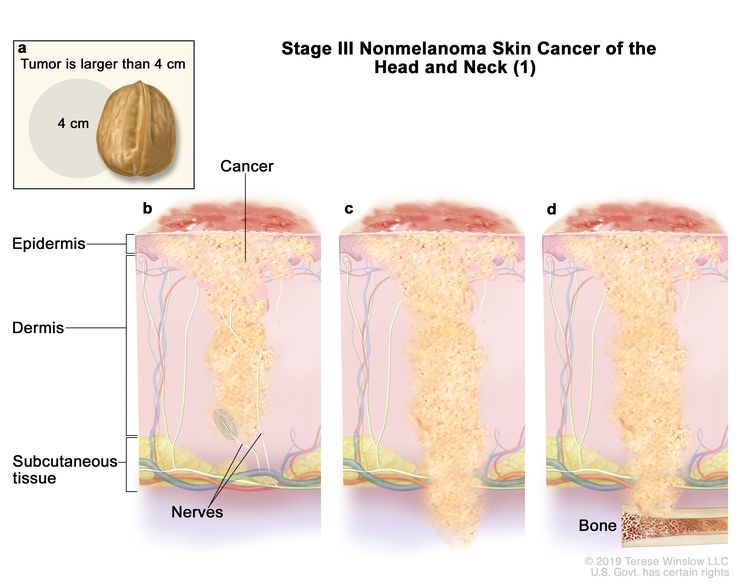
\includegraphics[width=0.7\textwidth]{imatges/problem_domain/stage3-skin-cancer.jpg}
\caption[Skin Cancer, Stage IV]{\textit{Skin Cancer, Stage IV. The tumor is larger than 2-4 centimeters and start spreading. Illustration by Terese Winslow}}
{\label{fig:stage3-skin-canceer}}
\end{figure}

\newpage

\subsection{Associated Factors and Preventions of Skin Cancer}

The risk factors associated with skin cancer encompass sun exposure, fair skin, as well as certain physical characteristics such as blond hair and blue eyes. The presence of melanin, a protein responsible for the skin's color or pigment, plays a crucial role in shielding the skin from ultraviolet (UV) radiation. Consequently, individuals with lighter skin or lower levels of melanin possess reduced UV protection \cite{OrigenAndTreatment}. \\

Although skin cancer may initially appear to predominantly affect individuals with light complexions, those with dark skin are also susceptible. They may observe signs of cancer on the palms of their hands or soles of their feet. \\

Advancements in research have led to treatments targeting the genetic level. New drug therapies assist in stimulating the immune system to produce antibodies capable of combatting rapidly dividing cells. While these therapies may have potential side effects, they are generally milder than those associated with chemotherapy. Moreover, they result in an enhanced immune system that is better equipped to battle cancer. \\

A patient's overall health also appears to influence their ability to fight cancer, although the precise connection between one's health and their risk of developing cancer remains unclear. However, it can be assumed that better overall health enhances the immune system's capacity to combat cancer. \\

Prevention of skin cancer is straightforward: minimizing exposure to the sun and UV radiation. Ceasing the use of tanning beds is advised. When exposed to the sun, wearing sunscreen and a wide-brimmed hat that provides comprehensive head shading is recommended \cite{OrigenAndTreatment}. \\

Consideration should also be given to wearing clothing with SPF protection. Some clothing manufacturers now produce summer attire with SPF levels similar to those found in sunscreen. This is significant since most regular t-shirts offer only minimal SPF protection of around 2. \\

Skin cancer ranks among the most prevalent forms of cancer, yet it is also one of the most easily detectable and treatable. Taking proactive measures to prevent sun exposure is crucial, while early detection is highly important. The prognosis is favorable when melanoma is identified in its early stages.




\chapter{Preliminaries}
\label{cap:prelim}

The objective of this chapter is to provide a comprehensive overview that defines the scope of the thesis. It covers essential theoretical concepts necessary to comprehend the experiments presented in subsequent chapters, delves into the technical knowledge required to understand the functioning of the CAD infrastructure, and explores the study of the dataset used for conducting the thesis.

\section{Theoretical Background}

This section provides an introduction to the theoretical foundations of training deep learning models. We will cover essential concepts such as neural networks, activation functions, loss functions, gradient descent. Understanding these concepts is crucial for comprehending the inner workings of deep learning algorithms and to know if the trained thesis models are performing correctly.

\subsection{Artificial Intelligence}

\textit{AI} is one of the newest fields in science and engineering. Work started in earnest soon
after World War II, and the name itself was coined in 1956 attributed by John McCarthy of MIT. \\

After successfully decrypting Enigma\footnote{Enigma was a rotor machine designed to encrypt and decrypt messages.}, in World War II, the mathematician Alan Turing posed a groundbreaking question that had a profound impact on society: "Can machines think?" \cite{CanMachineThink}. In this seminal work, Turing not only outlined the process of developing intelligent machines but also presented a method for assessing their intelligence. Even today, the Turing Test remains a widely recognized benchmark for evaluating the intelligence of artificial systems. According to this test, if a human cannot distinguish, through a text-based conversation, whether they are interacting with a human or a machine, the artificial system can be considered to possess intelligence. \\

The term "AI" is exciting but, the definition of this term is blurry \cite{AIModernApprouch}.
Historically there are two approaches to \textit{AI} that have been followed, each by different people
with different methods. The human-centered approach and the rationalist approach. The incorporation of a human-centered approach into the field must incorporate empirical scientific methods, which entail making observations and formulating hypotheses about human behavior. On the other hand, a rationalist approach combines the disciplines of mathematics and engineering. These different perspectives have both faced criticism and received praises. \\

From that juncture until the turn of the century, the field of \textit{AI} encountered fluctuations, witnessing periods of remarkable accomplishments interspersed with the infamous \textit{AI} winters. Currently \textit{AI} is a hot topic of discussion, evident from the increasing searches and online mentions. While \textit{AI} has been around for more than 65 years, the recent exponential trend can be attributed to the availability of cost-efficient storage, transfer, and computation capabilities for massive amounts of data. This newfound capacity was previously unimaginable and has contributed to the current \textit{AI} boom. \\

\newpage

\textit{AI} has expanded into numerous distinct fields, showcasing its extensive range of applications, techniques, and interdisciplinary nature. The diversity of branches in the field of artificial intelligence is represented in \textit{Figure \ref{fig:ai_branches}}, which depicts several current \textit{AI} fields. However, it is important to note that the figure can be further expanded to include additional fields, such as Speech Processing and Expert Systems, among others.

\begin{figure}[H]
\centering
\resizebox{0.8\textwidth}{!}{%
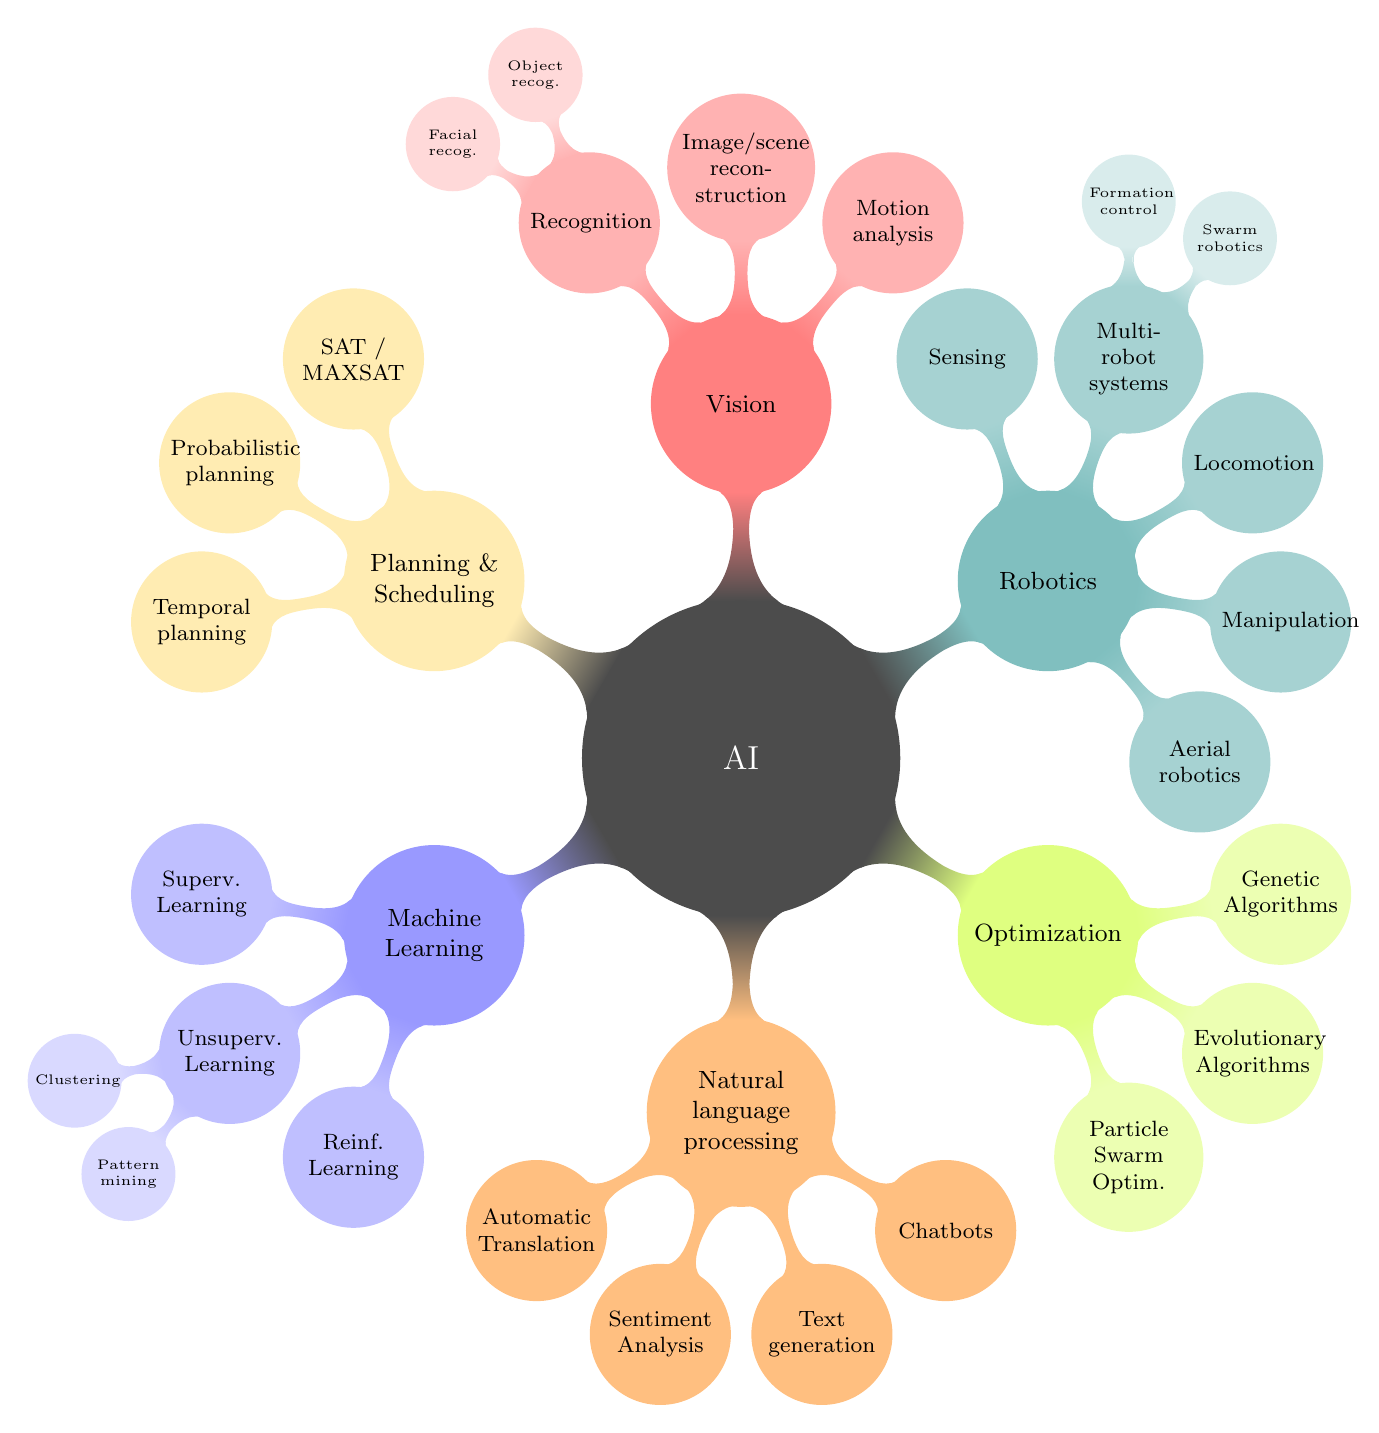
\begin{tikzpicture}[mindmap, grow cyclic, every node/.style=concept, concept color=black!70, text = white,
    level 1/.append style={level distance=4.5cm,sibling angle=60},
    level 2/.append style={level distance=3cm,sibling angle=40},
    level 3/.append style={level distance=2cm,sibling angle=40}]

\node{AI}
    child [concept color=blue!40, text = black] { node {Machine Learning}
        child [concept color=blue!25]{ node {Superv. Learning}}
        child [concept color=blue!25]{ node {Unsuperv. Learning}
            child [concept color=blue!15]{ node {Clustering}}
            child [concept color=blue!15]{ node {Pattern mining}}
        }
        child [concept color=blue!25]{ node {Reinf. Learning}}
    }
    child [concept color=orange!50, text = black] { node {Natural language processing}
        child { node {Automatic Translation}}
        child { node {Sentiment Analysis}}
        child { node {Text generation}}
        child { node {Chatbots}}
    }
    child [concept color=lime!50, text = black] { node {Optimization}
        child [concept color=lime!30]{ node {Particle Swarm Optim.}}
        child [concept color=lime!30]{ node {Evolutionary Algorithms}}
        child [concept color=lime!30]{ node {Genetic Algorithms}}
    }
    child [concept color=teal!50, text = black] { node {Robotics}
        child [concept color=teal!35]{ node {Aerial robotics}}
        child [concept color=teal!35]{ node {Manipulation}}
        child [concept color=teal!35]{ node {Locomotion}}
        child [concept color=teal!35]{ node {Multi-robot systems}
            child [concept color=teal!15]{ node {Swarm robotics}}
            child [concept color=teal!15]{ node {Formation control}}
        }
        child [concept color=teal!35]{ node {Sensing}}
    }
    child [concept color=red!50, text = black] { node {Vision}
        child [concept color=red!30]{ node {Motion analysis}}
        child [concept color=red!30]{ node {Image/scene reconstruction}}
        child [concept color=red!30]{ node {Recognition}
            child [concept color=red!15]{ node {Object recog.}}
            child [concept color=red!15]{ node {Facial recog.}}
        }
    }
    child [concept color=amber!30, text = black] { node {Planning \& Scheduling}
        child { node {SAT / MAXSAT}}
        child { node {Probabilistic planning}}
        child { node {Temporal planning}}
    };
\end{tikzpicture}%
}
\caption[AI Sub-Specialists]{\textit{\textit{AI} Sub-Specialists. Note that these subfields often intersect and combine. Illustration by Author}}
{\label{fig:ai_branches}}
\end{figure}

\newpage

\subsection{Machine Learning}

Machine learning is a branch of artificial intelligence (\textit{AI}) and computer science which focuses on the use of data and algorithms to imitate the way that humans learn, gradually improving its accuracy \cite{IBMMachineLearning}. The term \textit{AI} was defined by the pioneer Arthur Samuel as “the field of study that gives computers the ability to learn without explicitly being programmed.” \\

The central idea of machine learning is the existence of a mathematical relationship between any combination of input and output data. Rather than manually programming knowledge into computers, machine learning endeavors to automatically learn significant relationships and patterns by observing examples. \\

There are three subcategories of machine learning \cite{MITML}. These subcategories are listed bellow. \\

\vspace{0.5cm}
\textbf{Supervised Learning} \\

Machine learning models are trained with labeled data sets, which allow the models to learn and grow more accurate over time. For example, an algorithm would be trained with pictures of dogs and other things, all labeled by humans, and the machine would learn ways to identify pictures of dogs on its own. Supervised machine learning is the most common type used today. \\

\vspace{0.5cm}
\textbf{Unsupervised Learning} \\

Unsupervised learning involves using a training set that comprises unlabeled inputs, meaning inputs that do not have any assigned desired output. The primary objective of this learning approach is to uncover concealed patterns or data clusters without relying on human intervention. \\

\vspace{0.5cm}
\textbf{Reinforcement Learning} \\

Reinforcement learning occupies a position between supervised and unsupervised learning. In a certain sense, there is some form of supervision, but it does not involve explicitly specifying a desired output for every input in the data. Instead, a reinforcement learning algorithm receives feedback from the environment only after selecting an output, known as an action, based on a given input or observation. The feedback indicates the extent to which the action fulfills the learner's goals. \\

\textit{Figure \ref{fig:ml_branches}} is graphical representation of the subcategories of machine learning.

\begin{figure}[H]
\centering
\resizebox{0.65\textwidth}{!}{%
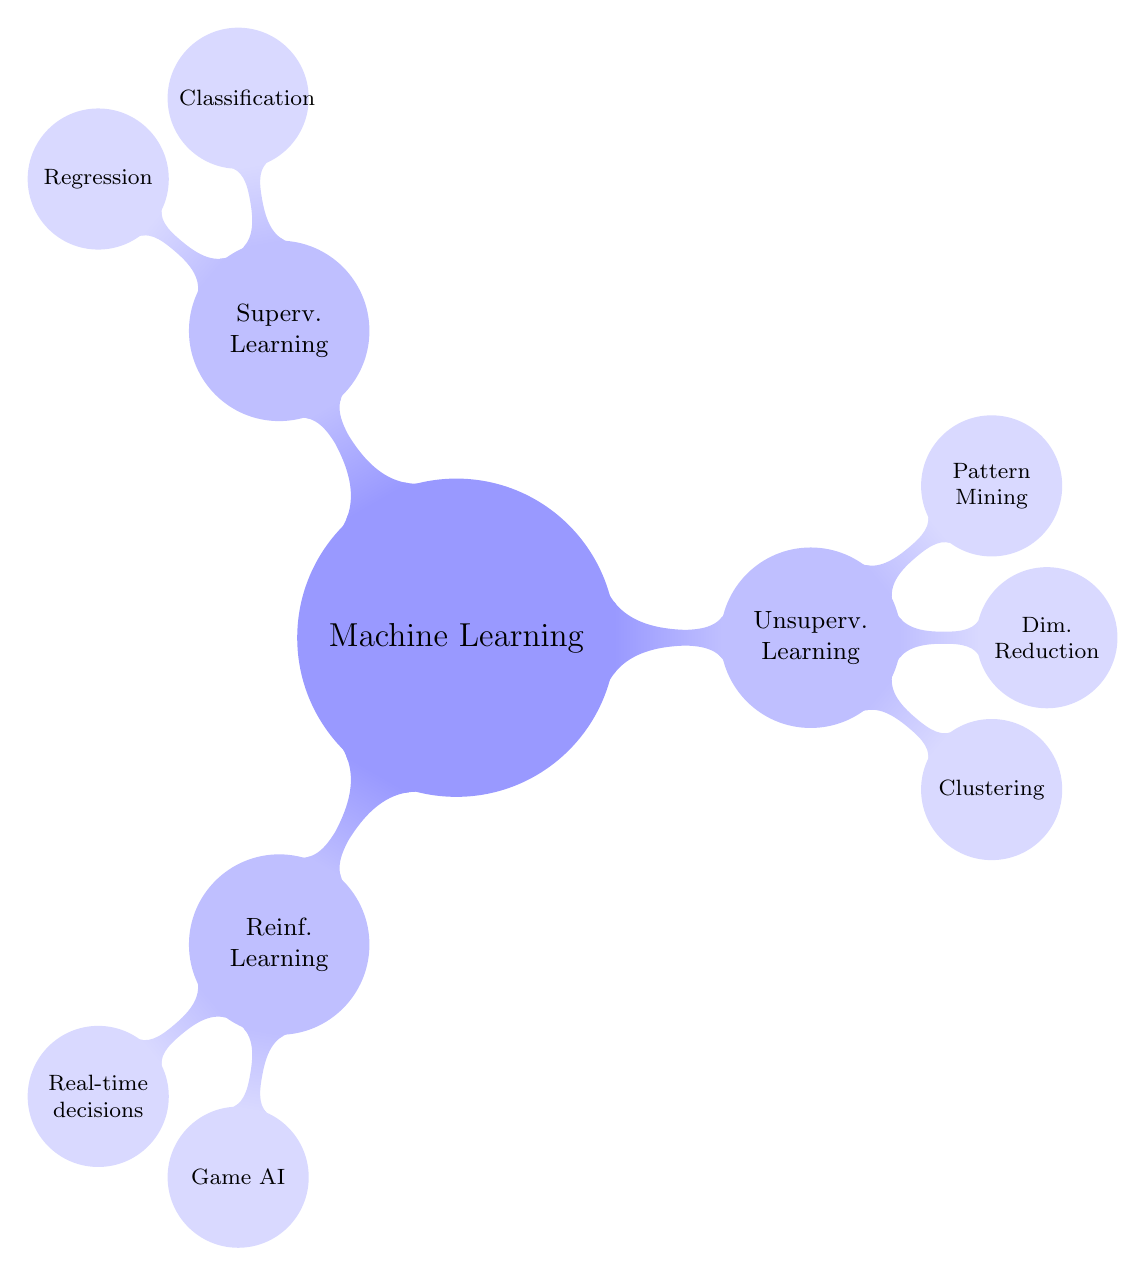
\begin{tikzpicture}[mindmap, grow cyclic, every node/.style=concept, concept color=blue!40, text = black,
    level 1/.append style={level distance=4.5cm,sibling angle=120},
    level 2/.append style={level distance=3cm,sibling angle=40},
    level 3/.append style={level distance=2cm,sibling angle=40}]

\node{Machine Learning}
    child [concept color=blue!25, text = black] { node {Reinf. Learning}
        child [concept color=blue!15]{ node {Real-time decisions}}
        child [concept color=blue!15]{ node {Game AI}}
    }
    child [concept color=blue!25, text = black] { node {Unsuperv. Learning}
        child [concept color=blue!15]{ node {Clustering}}
        child [concept color=blue!15]{ node {Dim. Reduction}}
        child [concept color=blue!15]{ node {Pattern Mining}}
    }
    child [concept color=blue!25, text = black] { node {Superv. Learning}
        child [concept color=blue!15]{ node {Classification}}
        child [concept color=blue!15]{ node {Regression}}
    };
\end{tikzpicture}%
}
\caption[Subcategories of Machine Learning.]{\textit{Subcategories of Machine Learning. Illustration by Author}}
{\label{fig:ml_branches}}
\end{figure}


\subsection{Deep Learning}

Deep learning, is a subset of machine learning algorithms, is primarily associated with supervised learning techniques. This algorithms derive conclusions by analyzing data with a given logical structure. In contrast to traditional machine learning algorithms, deep learning algorithms operate at a higher level of abstraction. They possess the ability to perform the laborious process of feature extraction. Each algorithm applies a nonlinear transformation to its input and uses the acquired knowledge to generate a statistical model as the output. This iterative process continues until the output reaches an acceptable level of accuracy. The term "deep" refers to the number of layers the data must pass through during these iterations. \\

Deep learning has been successfully applied to various problems, ranging from self-driving cars to speech recognition. In this particular project, deep learning is employed to classify whether a given dermoscopy image is a melanoma or not. To achieve this, it has been necessary to understand how convolutional neural networks work, address certain issues that affect the precision of these models, explain the key metrics primarily used to measure the accuracy of these models.


\subsection{Deep Neural Networks}

Deep neural networks are part of the deep learning algorithms within the realm of machine learning, which, as mentioned earlier, falls under the umbrella of artificial intelligence. \textit{Figure \ref{fig:deep-learning-family}} is an illustration of the deep learning family. \\

\begin{figure}[H]
\centering
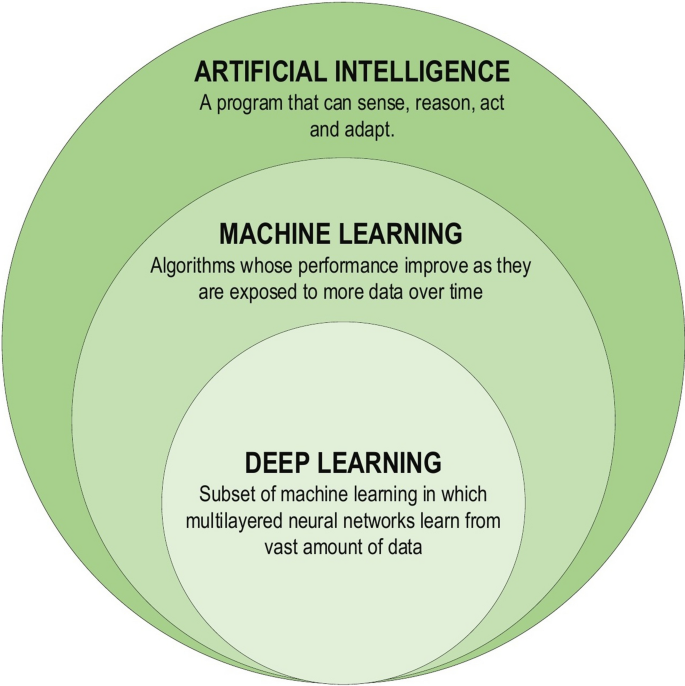
\includegraphics[width=0.6\textwidth]{imatges/preliminaries/deep-learning-familiy.png}
\caption[Deep Learning Family]{\textit{Deep Learning Family. Illustration by towardsdatascience}}
{\label{fig:deep-learning-family}}
\end{figure}

Deep neural networks, also known as fully connected layers, are modeled after the human brain. These algorithms achieve their functionality by propagating signals from the input layer to the output layer while passing through intermediate hidden layers. Each layer consists of neurons responsible for detecting patterns from the incoming connections. These neurons perform a crucial task by combining input from the data with a corresponding set of coefficients, also known as weights. These weights act as amplifiers or dampeners, modulating the impact of the input on the neuron's activation. \\

By leveraging this mechanism, each layer in the deep neural network acquires the capability to capture distinctive features from the input data. Notably, as the signal travels deeper into the network, the extracted features become increasingly sophisticated and abstract. This characteristic arises from the hierarchical nature of the network architecture, enabling the model to learn and discern intricate patterns and representations. \\

The process of feature extraction in deep neural networks allows the network to progressively learn and uncover complex relationships within the data. As the signal traverses through the network's layers, each subsequent layer builds upon the extracted features from the previous layer, resulting in the generation of more intricate and comprehensive representations. This ability to capture and model hierarchical features is a significant advantage of deep neural networks, making them particularly effective in tasks requiring the recognition of complex patterns and high-level abstractions.

\begin{figure}[H]
\centering
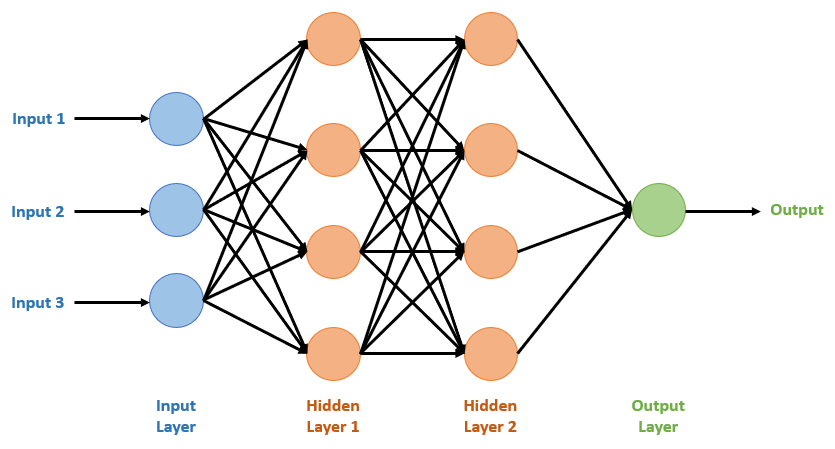
\includegraphics[width=0.8\textwidth]{imatges/preliminaries/deep-neural-network.png}
\caption[Deep Neural Network]{\textit{Deep Neural Network. This NN has two hidden layers. Illustration by Introduction to Neural Networks in Deep Learning}}
{\label{fig:deep-nn}}
\end{figure}

The minimum unit in a layer is known as neuron or perceptron.
The perceptron, is the oldest simple neural network, created by Frank Rosenblatt in 1958.
Every node within the network possesses an associated value, which is computed based on the incoming nodes and edges,
as depicted in \textit{Figure \ref{fig:perceptron}}. The computation takes place in the following manner: the products
of  inputs and their respective weights are summed with a bias, and this sum is subsequently passed through the node's activation function.
The activation function serves the purpose of compressing the resulting value within the range of 0 to 1 and introduces non-linearity,
allowing the model to learn complex relationships in the data. The resulting value determines the
degree to which the signal should propagate through the network, ultimately influencing the final outcome.

\begin{figure}[H]
\centering
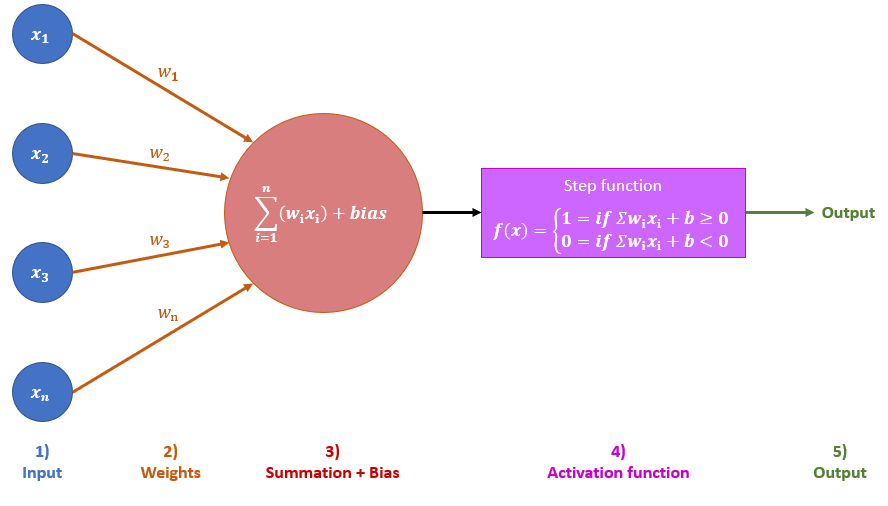
\includegraphics[width=0.75\textwidth]{imatges/preliminaries/perceptron.png}
\caption[The Perceptron]{\textit{The Perceptron. Illustration by Introduction to Neural Networks in Deep Learning}}
{\label{fig:perceptron}}
\end{figure}


\subsection{Convolutional Neural Networks}

A convolutional neural network (CNN) is a specific type of neural network that is particularly well-suited for analyzing visual imagery. It draws inspiration from the organization of the animal visual cortex, which is responsible for visual processing in living organisms. \\

One of the key innovations of CNNs is their ability to automatically learn a large number of filters in parallel. These filters are learned during the training process and are specifically tailored to solve a particular predictive modeling problem, such as image classification. By learning these filters, CNNs become adept at extracting relevant features and patterns from visual data without the need for manual feature engineering. \\

CNNs are designed to learn spatial hierarchies of features through a process called backpropagation. During training, the network adapts its internal parameters, or weights, by iteratively propagating the error backwards from the output to the input layers. This allows the network to gradually adjust its weights in a way that minimizes the difference between its predicted outputs and the true outputs. \\

One key distinction of CNNs compared to regular neural networks is their use of parameter sharing. In a CNN, all neurons within a particular feature map share the same weights. This sharing of weights significantly reduces the number of parameters in the network, making it more computationally efficient. By sharing weights, the network can detect the same patterns or features regardless of their spatial position in the input data. This property, known as translation invariance, enables CNNs to recognize objects or patterns regardless of their location within an image.\\

Furthermore, CNNs have a three-dimensional arrangement of neurons: width, height, and depth. The width and height dimensions correspond to the spatial dimensions of the input data, such as the width and height of an image. The depth dimension refers to the number of channels or feature maps in each layer, where each channel represents a different aspect or feature of the input. \\

To build CNN architectures, there are four main types of layers used, and they are listed bellow. \\

\newpage

\vspace{0.5cm}
\textbf{Convolutional Layers} \\

A convolutional layer is responsible for detecting and extracting features from the input data. It consists of a set of learnable filters, also known as kernels or feature detectors. Each filter is a small matrix of weights that slides or convolves across the input data to perform a dot product operation at each spatial location.  \\

The filter slides or convolves across the input data with a defined stride, which specifies the amount of shift between each position.
At each spatial location, a dot product is computed between the filter and the overlapping region of the input.
The dot product involves element-wise multiplication of the filter values with the corresponding input values, followed by summing up the results. \\

The result of each dot product operation is a single value, forming a pixel in the output feature map. Additionally, an activation function is applied element-wise to introduce non-linearity into the network. \\

\begin{figure}[H]
\centering
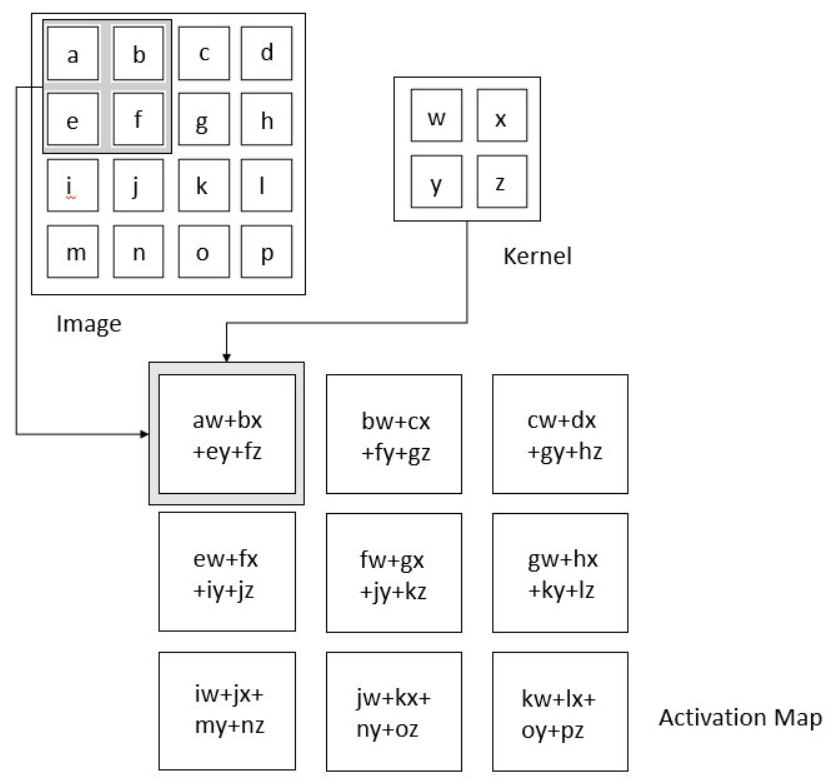
\includegraphics[width=0.8\textwidth]{imatges/preliminaries/convolutional-layer.png}
\caption[Convolutional Operation on Input Image]{\textit{Convolutional Operation on Input Image. Illustration by towardsdatascience}}
{\label{fig:convoluional-layer}}
\end{figure}

\newpage

\vspace{0.5cm}
\textbf{Pooling Layers} \\

Pooling layers performs a summarizing of nearby outputs in the network, effectively replacing certain locations with a condensed representation. This reduces the spatial dimensionality of the output, leading to decreased computational requirements and weight parameters. The pooling operation is applied independently to each slice of the representation. \\

Various pooling functions exist, including averaging the values within a rectangular neighborhood, computing the L2 norm of the neighborhood, or using a weighted average based on distance. However, the most widely used method is max pooling, which selects the maximum output value from the neighborhood.

\begin{figure}[H]
\centering
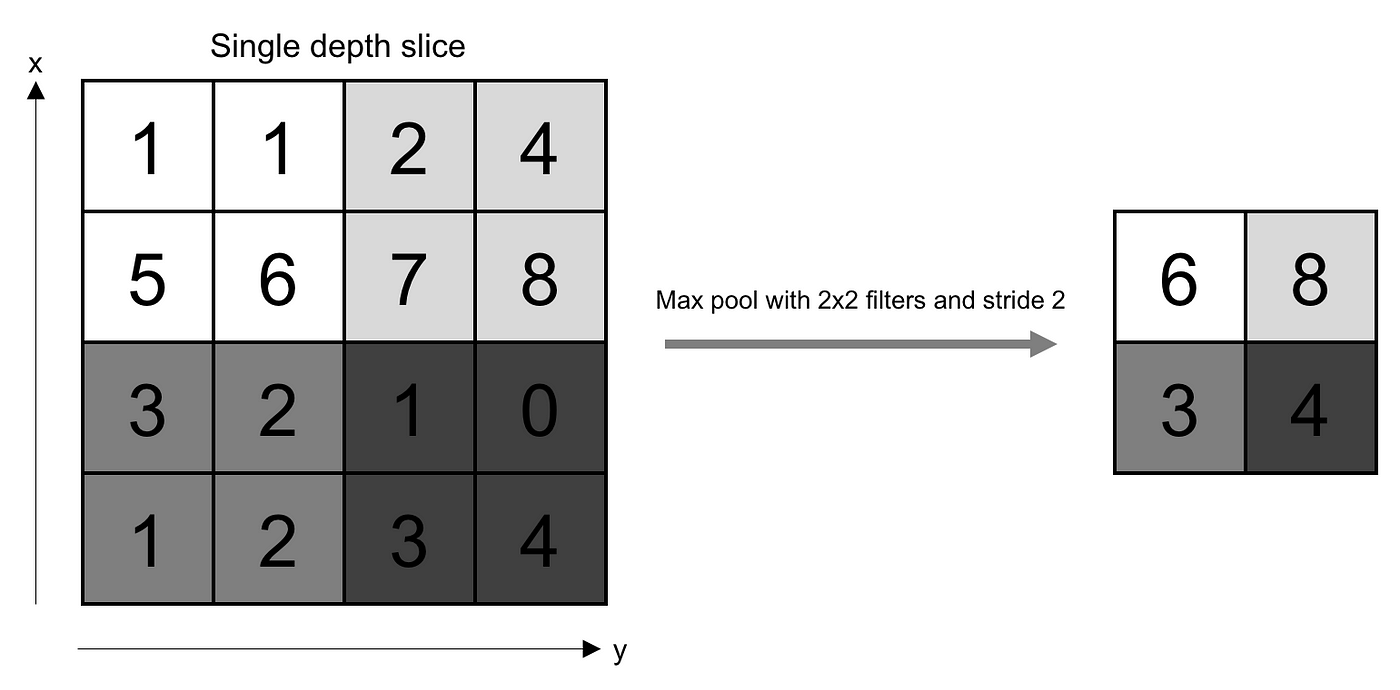
\includegraphics[width=0.8\textwidth]{imatges/preliminaries/polling-layer.png}
\caption[Polling Operation on Input Image]{\textit{Polling Operation on Input Image. Illustration by towardsdatascience}}
{\label{fig:polling-layer}}
\end{figure}

\vspace{0.5cm}
\textbf{Fully Connected Layers} \\

Neurons in this layer have full connectivity with all neurons in the preceding and succeeding layer. This is why it can be computed as usual by a matrix multiplication followed by a bias effect. The topology in the fully connected portion of a CNN depends on various factors, including the complexity of the task, the nature of the data, and the capacity of the model. There is no fixed rule for determining the exact number of neurons or layers, and it often requires experimentation and tuning. \\

The fully connected layer helps to map the representation between the input and the output. See \textit{Figure \ref{fig:deep-nn}} to a visual representation of a fully connected layer. \\

\vspace{0.5cm}
\textbf{Non-linearity Layers} \\

Convolutional operations in neural networks are linear, meaning they capture linear patterns in the data. However, many objects in images exhibit non-linear characteristics that cannot be effectively detected using linear operations alone. To address this limitation, non-linearity layers, such as activation functions, are typically applied immediately after the convolutional layer. These non-linearity layers introduce non-linear transformations to the activation maps, enabling the network to learn and detect complex, non-linear patterns in the data. \\

There are many types of non-linearity functions applied after the convolutional layers, the most popular are: \\

\begin{itemize}

\item \textbf{Sigmoid}

The sigmoid function takes a real-valued number and “squashes” it into a range between 0 and 1.

\centering {
\begin{tikzpicture}
  \draw[->] (-5,0) -- (5,0) node[right] {$x$};
  \draw[->] (0,-0.5) -- (0,1.5) node[above] {$\sigma(x)$};
  \draw[domain=-5:5, smooth, variable=\x, blue] plot (\x, {1/(1 + exp(-\x))});
  \draw[dashed] (-5, 0.0) node[left] {0};
  \draw[dashed] (-5, 1) node[left] {1} -- (5, 1);
\end{tikzpicture}
}

\raggedright
Mathematically, the sigmoid function is expressed as:

\[ \sigma(x) = \frac{1}{1 + e^{-x}} \]

\item \textbf{ReLU}

The Rectified Linear Unit (ReLU) is maybe the most popular activation functions in the last few years. The function is just simply threshold at zero.

\centering
\begin{tikzpicture}
  \draw[->] (-5,0) -- (5,0) node[right] {$x$};
  \draw[->] (0,-0.5) -- (0,5) node[above] {$\text{ReLU}(x)$};
  \draw[domain=-5:0, smooth, variable=\x, blue] plot (\x, 0);
  \draw[domain=0:5, smooth, variable=\x, blue] plot (\x, \x);
  \draw[dashed] (-5, 0.0) node[left] {0};
    \draw[dashed] (-5, 1) node[left] {1} -- (5, 1);
\end{tikzpicture}

\raggedright
Mathematically, the ReLU function is expressed as:

\[f(x) = \max(0, x)\]

\item \textbf{Tanh}

The hyperbolic tangent function tanh compresses a real-valued number to the range of [-1, 1]. Similar to the sigmoid function, tanh exhibits saturation, but unlike sigmoid, its output is centered around zero.

\centering
\begin{tikzpicture}
  \draw[->] (-5,0) -- (5,0) node[right] {$x$};
  \draw[->] (0,-1.5) -- (0,1.5) node[above] {$\tanh(x)$};
  \draw[domain=-5:5, smooth, variable=\x, blue] plot (\x, {tanh(\x)});
  \draw[dashed] (-5, -1) node[left] {-1} -- (5, -1);
  \draw[dashed] (-5, 1) node[left] {1} -- (5, 1);
\end{tikzpicture}

\raggedright
Mathematically, the tanh function is expressed as:

\[ \tanh(x) = \frac{{e^x - e^{-x}}}{{e^x + e^{-x}}} \]

\end{itemize}

\subsection{Loss Function}

A loss function, also known as a cost function or an objective function, is a measure used in machine learning and optimization algorithms to quantify how well a model performs on a given task. It represents the discrepancy between the predicted outputs of a model and the true values or labels associated with the training data. \\

Different machine learning tasks and algorithms may use different loss functions, depending on the specific problem being addressed. Commonly used loss functions include:

\begin{itemize}
    \item Mean Squared Error (MSE)
    \item Binary Cross-Entropy
    \item Mean Absolute Error (MAE)
    \item Cross-entropy Loss
\end{itemize}

For this thesis, the loss function used to train the models is
{\tt Cross-entropy Loss} as this is a multiclass problem. Don't confuse the optimizer
algorithm with the metric used to evaluate how good models are.
We used the ROC AUC with one-vs-rest strategy to evaluate the models performance, explained in \textit{Section \ref{sec:metrics}}. \\

Cross-entropy loss, also known as log loss, is a widely used loss function in machine learning, particularly in classification tasks. It measures the dissimilarity between predicted class probabilities and true class labels. \\

In multi-class classification, the cross-entropy loss is calculated using the true class labels \(y\) and the predicted class probabilities \(p\) for each class. It can be defined as:

\[-\sum_{i=1}^{C} y_i \log(p_i)\]

\noindent where:

\begin{itemize}
    \item \(C\) is the total number of classes.
    \item \(y_i\) represents the true label for class \(i\).
    \item \(p_i\) represents the predicted probability for class \(i\).
\end{itemize}

\newpage

\subsection{Metrics}
{\label{sec:metrics}}

There are various metrics commonly used to assess the quality of a model's predictions.
In this section, we present a selection of metrics that we find relevant for evaluating our models.

\vspace{0.5cm}
\textbf{Confusion Matrix} \\

\noindent A confusion matrix is a square matrix with dimensions {\tt NxN}, where {\tt N} represents the total number of classes being predicted. It provides a visual representation of the errors or confusion made by a classification model during its predictions. The matrix, illustrated as \textit{Figure \ref{fig:confusion-matrix}}, is structured with columns and rows representing the predicted and actual classes, respectively.

\begin{figure}[H]
\begin{adjustbox}{trim={0pt 0.5cm 0pt 1cm}, clip}
\centering
\includegraphics[width=0.9\textwidth]{imatges/preliminaries/confusion-matrix.png}
\end{adjustbox}
\caption[Confusion Matrix Multi-Class]{\textit{Confusion Matrix Multi-Class. Illustration by WIKIPEDIA}}
{\label{fig:confusion-matrix}}
\end{figure}

\begin{itemize}
\item \textbf{True Positive (TP)}

This refers to an outcome where the model accurately predicts the positive class.
\item \textbf{False Positive (FP)}

This describes a situation where the model mistakenly predicts the positive class when it should have predicted the negative class.
\item \textbf{True Negative (TN)}

This represents an outcome where the model correctly predicts the negative class.
\item \textbf{False Negative (FN)}

This indicates a scenario where the model incorrectly predicts the negative class instead of predicting the positive class.

\end{itemize}

In a logical sense, when we add up the elements on the main diagonal of the confusion matrix,
we obtain the total number of correct predictions.
Conversely, summing the elements on the antidiagonal provides us with the total number of incorrect predictions.
Utilizing these values, we can compute additional metrics such as accuracy, precision, recall, specificity, and F1 score. \\

\vspace{0.5cm}
\textbf{Accuracy} \\

\noindent Accuracy is a commonly employed and straightforward performance metric in classification tasks. It calculates the ratio of correct predictions to the total number of predictions made on a dataset, thus determining the likelihood of correctly classifying an input. Accuracy is especially valuable when working with a balanced dataset, where the number of instances in each class is roughly equivalent. However, in the case of the previously mentioned thesis dataset, which is not balanced, the use of accuracy serves primarily to monitor model training performance rather than being the main evaluation metric.

\[Accuracy = \frac{TP + TN}{TP + TN + FP + FN}\]

\vspace{0.5cm}
\textbf{TPR} \\

TPR stands for True Positive Rate, and it is also known as sensitivity or recall.
It measures the proportion of actual positive cases that are correctly identified as positive
by a classification model or test.

\[
\text{TPR} = \frac{\text{TP}}{\text{TP} + \text{FN}}
\]

\vspace{0.5cm}
\textbf{FPR} \\

FPR stands for False Positive Rate, and it measures the proportion of actual negative cases that are incorrectly identified as positive by a classification model or test.

\[
\text{FPR} = \frac{\text{FP}}{\text{FP} + \text{TN}}
\]

\vspace{0.5cm}
\textbf{AUC-ROC Curve with One-vs-Rest Strategy} \\

The ROC Curve, when computed with the one-vs-rest (OvR) strategy for multiclass classification, provides insights into how well the model can differentiate a class from the rest of the classes. It is a probabilistic curve that plots the true positive rate (TPR) against the false positive rate (FPR). By treating the target class as the positive class and the remaining classes as the negative class in separate binary classification tasks (\textit{Figure \ref{fig:auc-roc}}). \\

The area under the curve (AUC) is a value between 0 and 1 that measures
the ability of a classifier to distinguish between classes. It is used as a summary
of the ROC curve. The higher the AUC, the better the performance of the
model at distinguishing between the positive and negative classes.

\begin{figure}[H]
\centering
\includegraphics[width=0.8\textwidth]{imatges/preliminaries/auc.png}
    \caption[Forward Propagation and Backward Propagation]{\textit{AUC-ROC. Comparison of multiple ROC curves and how much overlap there are between classes. Illustration by Elizabeth Louise Thomas}}
{\label{fig:auc-roc}}
\end{figure}


\subsection{Optimizer}

An optimizer is an algorithm that finds the value of the parameters (weights) that minimize the error when mapping inputs to outputs. These optimization algorithms widely affect the accuracy and speed training of the deep learning models. \\

While training a deep learning models, the optimizer modifies the weights of the model in each epoch to minimize the loss function. \\

The are a considerable amount of different optimizer algorithms out there with their pros and cons. In this section I present the family of optimizers based on Gradient Descent optimization. This family of optimizer algorithms were used for the thesis. \\

\vspace{0.5cm}
\textbf{Gradient Descent} \\

Using the Gradient Decent optimization algorithm, the weights are updated incrementally after each epoch (pass over the training dataset). \\

The magnitude and direction of the weight update is computed by taking a step in the opposite direction of the cost gradient.

\[\nabla J(w) = (\frac{\partial J}{\partial w_1}, \frac{\partial J}{\partial w_2}, \ldots, \frac{\partial J}{\partial w_n})\]

\[
\Delta w = -\eta \cdot \nabla J(w)
\]

Finally, the weight are updated after each epoch with the following expression:

\[
w = w + \Delta w
\]


\begin{itemize}
    \item \(\Delta w\) represents the weight update.
    \item \(\eta\) (eta) denotes the learning rate, which controls the step size of the update.
    \item  \(\frac{\partial J}{\partial w_i}\) represents the partial derivative of the cost function \(J\) with respect to the weight \(w_i\).
    \item \(\nabla J(w)\) represents the gradient of the cost function \(J(w)\) with respect to the weights \(w\).
\end{itemize}

In Gradient Descent optimization, we compute the cost gradient based on the complete training set; hence, we sometimes also call it batch gradient descent. In case of very large datasets, using Gradient Descent can be quite costly since we are only taking a single step for one pass over the training set – thus, the larger the training set, the slower our algorithm updates the weights and the longer it may take until it converges to the global cost minimum. \\

\newpage

The next lines are a high level pseudo-implementation of the Gradient Descent algorithm:

\begin{itemize}[label=\(\circ\)]
  \item for each epoch:
  \begin{itemize}[label=\(\circ\), topsep=0pt]
    \item for each weight \(j\):
    \begin{itemize}[label=\(\circ\), topsep=5pt]
      \item \(w_j = w_{j-1} + \Delta w_j\)
    \end{itemize}
  \end{itemize}
\end{itemize}

The \textit{Figure \ref{fig:optimization}} shows how the Gradient Descent optimizer would try to modify the  the weight values that minimizes the cost function.

\begin{figure}[H]
\centering
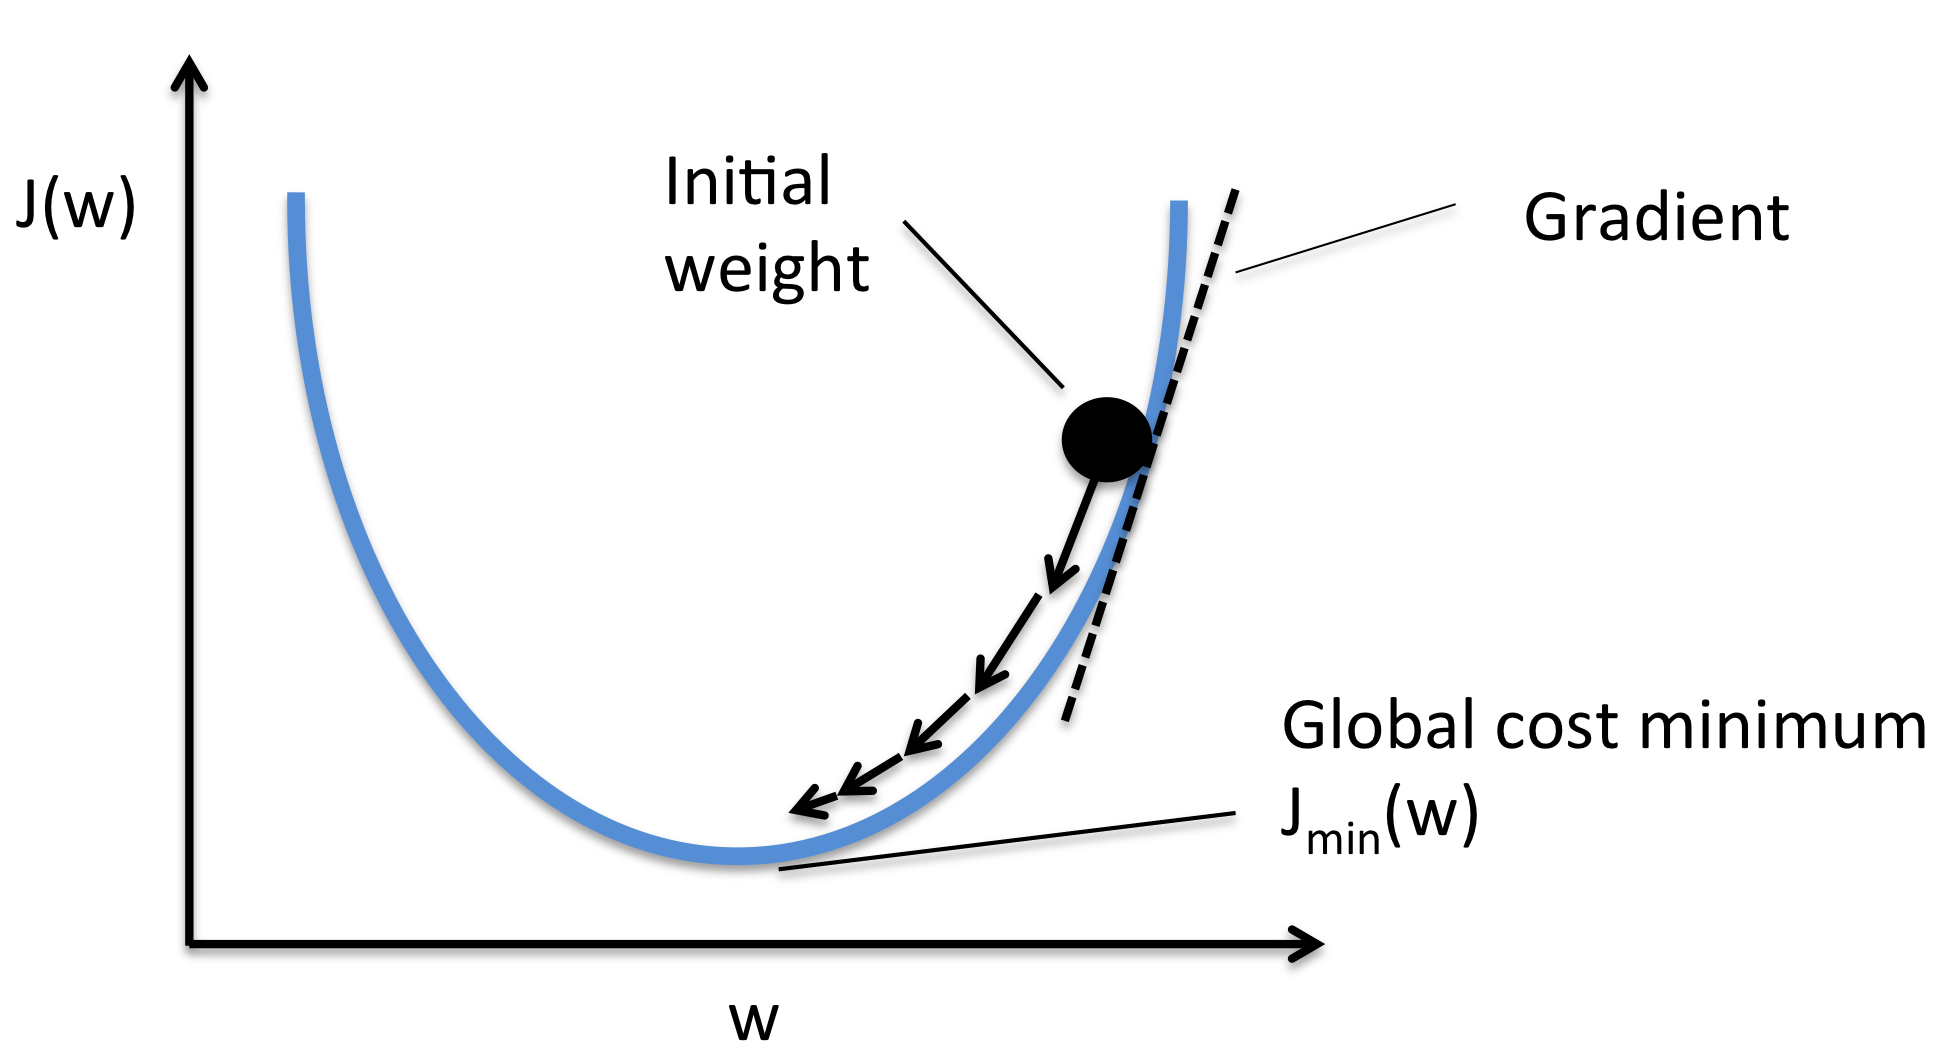
\includegraphics[width=0.7\textwidth]{imatges/preliminaries/optimization.png}
    \caption[Function Optimization]{\textit{Function Optimization. Optimization of a 2D function using Gradient Descent algorithm. Illustration by sebastianraschka}}
{\label{fig:optimization}}
\end{figure}

\vspace{0.5cm}
\textbf{Stochastic Gradient Descent} \\

Stochastic Gradient Descent work similar to the Gradient Descent but the weight updates are not accumulated as we’ve seen above for Gradient Descent. Instead, the weights are updated after each training sample. Due to its stochastic nature, the path towards the global cost minimum is not “direct” as in Gradient Descent, but may go “zig-zag”if we are visuallizing the cost surface in a 2D space, see \textit{Figure \ref{fig:sgdvsgd}}. However, it has been shown that Stochastic Gradient Descent almost surely converges to the global cost minimum if the cost function is convex. \\

\newpage

The next lines are a high level pseudo-implementation of the Stochastic Gradient Descent algorithm:

\begin{itemize}[label=$\circ$]
    \item for each epoch or until approx. cost minimum is reached:
        \begin{itemize}[label=$\circ$, topsep=0pt]
            \item for training sample \(i\):
              \begin{itemize}[label=$\circ$, topsep=5pt]
                \item for each weight \(j\):
                    \begin{itemize}[label=$\circ$, topsep=10pt]
                        \item \(w_j = w_{j-1} + \Delta w_j\), where \(\Delta w_j = \eta (target^{(i)} - output^{(i)})x_{j}^{(i)}\)
                    \end{itemize}
            \end{itemize}
        \end{itemize}
\end{itemize}

\begin{figure}[H]
\centering
\begin{adjustbox}{trim=0cm 0cm 0cm 1cm, clip}
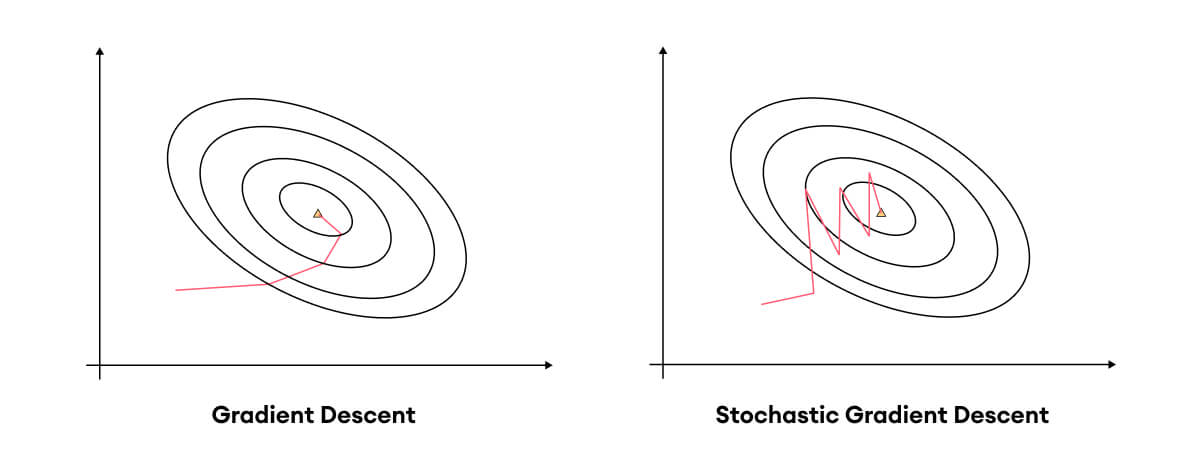
\includegraphics[width=0.9\textwidth]{imatges/preliminaries/sgdvsgd.jpeg}
\end{adjustbox}
    \caption[Gradient Descent vs Stochastic Gradient Descent]{\textit{Gradient Descent vs Stochastic Gradient Descent. It illustrates the optimization process of both algorithms. Illustration by superannotate}}
{\label{fig:sgdvsgd}}
\end{figure}

\subsection{Forward Propagation and Backward Propagation}

Forward and backpropagation are fundamental processes in training neural networks and optimizing their parameters. They play a crucial role in enabling the network to learn from data and improve its performance over time. \\

Resuming the forward-propagation and back-propagation (\textit{Figure \ref{fig:forward-and-back-propagation}}), in order to find the direction of the steepest descent (minimising the overall loss function), we need to calculate gradients of the loss function with respect to weights and bias. After that, we’ll be able to update weights and bias using negative gradients multiplied by the learning rate.

\begin{figure}[H]
\centering
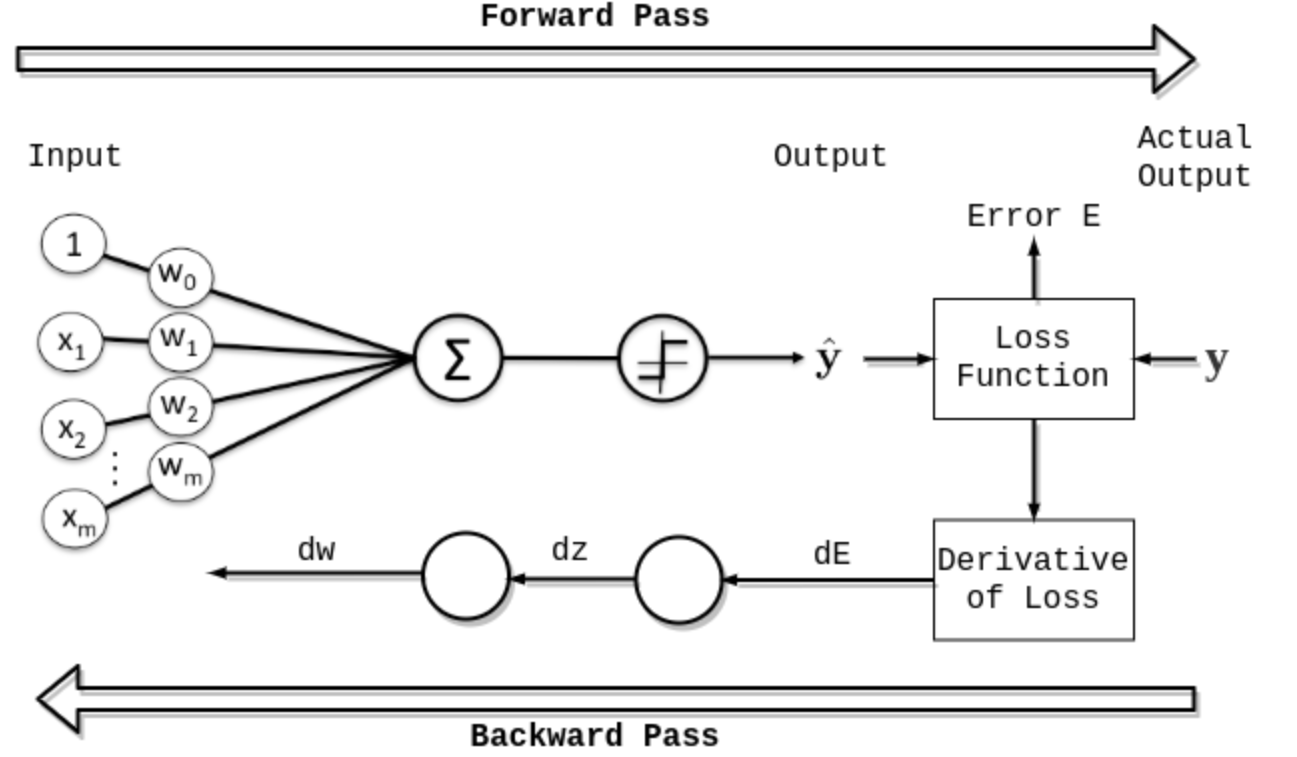
\includegraphics[width=0.8\textwidth]{imatges/preliminaries/front-and-back-prop.png}
    \caption[Forward Propagation and Backward Propagation]{\textit{Forward Propagation and Backward Propagation. Illustration by baeldung}}
{\label{fig:forward-and-back-propagation}}
\end{figure}

\vspace{0.5cm}
\textbf{Forward Propagation} \\

Forward propagation refers to the process of computing the output of a neural network given an input or a batch of inputs. During forward propagation, the input data flows through the network's layers in a sequential manner, from the input layer to the output layer. Each layer performs a series of computations, typically involving linear transformations (such as matrix multiplications) followed by activation functions. \\

As the data flows forward through the network, intermediate outputs, also known as activations or feature maps, are computed at each layer. These activations are then passed on as inputs to the subsequent layers until the final output is produced. The forward propagation process essentially calculates the predicted output of the network for a given input. \\

\vspace{0.5cm}
\textbf{Backward Propagation} \\

Backward propagation, short for backward propagation of errors, is the process of computing the gradients of the network's parameters with respect to a loss function. These gradients indicate the sensitivity of the network's output to changes in its parameters and are used to update the parameters during the training process. \\

The backward propagation algorithm starts from the final output of the network and propagates the error gradients backward through the network's layers. It computes the gradients layer by layer using the chain rule of calculus. The gradients quantify how each parameter contributed to the overall error of the network and provide information on how to adjust the parameters to reduce the error. \\

Once the gradients are computed, an optimization algorithm (such as stochastic gradient descent) uses them to update the network's parameters in a way that minimizes the loss function. The process of repeatedly performing forward propagation, computing gradients through back-propagation, and updating the parameters is carried out iteratively until the network converges to a desirable level of performance.


\subsection{Under-fitting vs Over-fitting}

Under-fitting is a prevalent challenge in machine learning, occurring when the model fails to establish a meaningful relationship between the input and target variable. Insufficiently capturing the features of the data results in increased errors in both the training and unseen data samples. \\

Over-fitting is also a prevalent challenge in machine learning but it is really common in deep learning algorithms. Deep learning models try to fit the training data entirely and ends up memorizing the data patterns and the noise/random fluctuations. These models fail to generalize and perform well in the case of unseen data scenarios, defeating the model's purpose. \\

\textit{Figure \ref{fig:underfitting-overfitting-goodfitting}} illustrates the under-fitting and over-fitting issue against a good fitting in a classifier problem.

\begin{figure}[H]
\centering
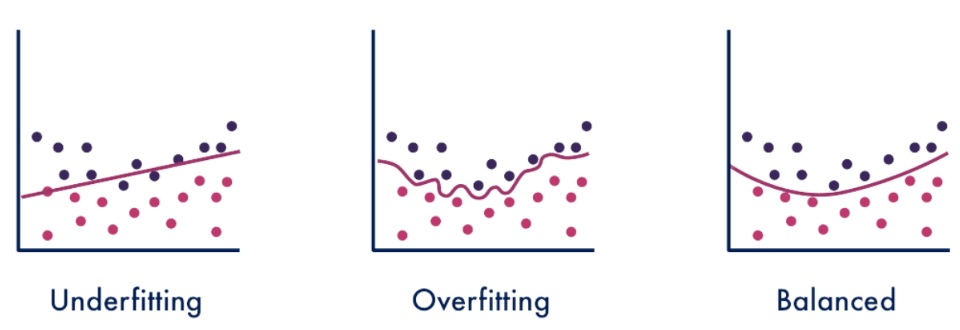
\includegraphics[width=0.9\textwidth]{imatges/preliminaries/over-under-base.jpg}
\caption[Under-fitting vs Over-fitting vs Good Fitting]{\textit{Under-fitting vs Over-fitting vs A Good Fitting. Illustration by towardsdatascience}}
{\label{fig:underfitting-overfitting-goodfitting}}
\end{figure}

\subsection{Strategies to Combat Over-fitting}

There are lot of strategies to combat over-fitting, in this section there is presented only those used in the project. \\

\vspace{0.5cm}
\textbf{Early Stopping} \\

Early Stopping involves monitoring the model's performance on a validation dataset during training. If the performance stops improving or starts deteriorating, the training process is stopped early. By doing this, early stopping helps find the optimal balance between model complexity and generalization, ensuring the model doesn't become overly specialized to the training data and does not performs well on unseen data. \\

\begin{figure}[H]
\centering
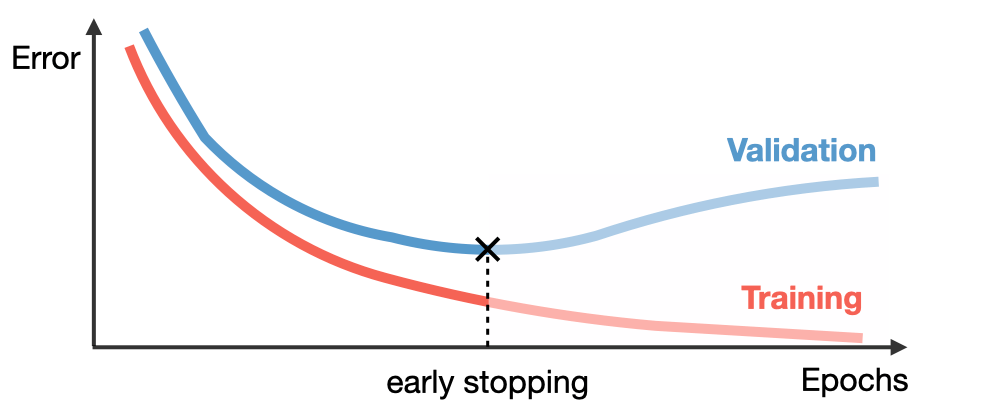
\includegraphics[width=0.7\textwidth]{imatges/preliminaries/early-stop.png}
\caption[Early Stopping]{\textit{Early Stopping. the vertical doted line represents the point where the early stop mechanism should have been triggered. Illustration by wandb}}
{\label{fig:early-stop}}
\end{figure}

\vspace{0.5cm}
\textbf{Learning Rate Scheduling} \\

The learning rate is a hyper-parameter in machine learning that determines the step size at which a model's parameters are updated during the optimization process. In most optimization algorithms, such as gradient descent, the learning rate controls how quickly or slowly the model learns from the training data. \\

There are various approaches in learning rate scheduling, bellow you'll find the scheduling used in the thesis.

\newpage

\begin{itemize}
    \item \textbf{Learning Rate Decay}

    This learning rate scheduling works gradually reducing the learning rate over time or in response to certain conditions. A smaller learning rate allows the model to fine-tune its parameters more cautiously, preventing it from aggressively fitting to noisy or irrelevant patterns in the training data. This smoother adjustment helps the model converge to a better generalize solution, reducing the risk of over-fitting.

    \begin{figure}[H]
    \centering
    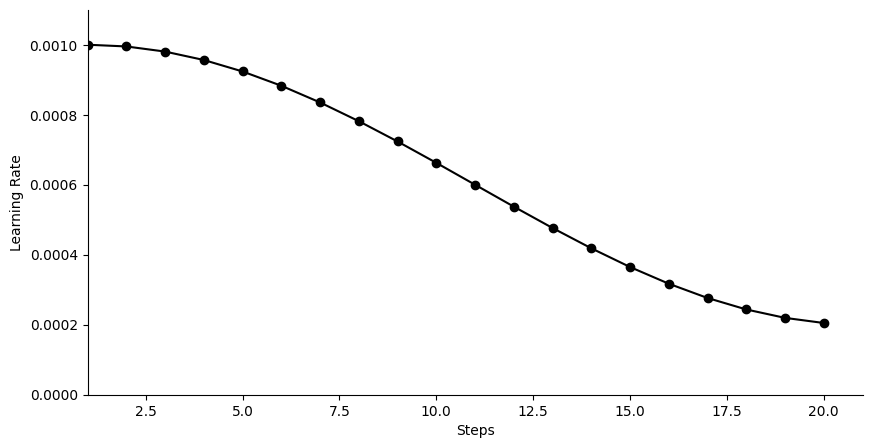
\includegraphics[width=0.6\textwidth]{imatges/preliminaries/learning-rate-decay.png}
    \caption[Learning Rate Decay]{\textit{Learning Rate Decay. In this graphic it's represented how the learning rate hyperparameter decrease over the epochs. Illustration by Author}}
    {\label{fig:learning-rate-decay}}
    \end{figure}

    \item \textbf{Cycling Learning}

    Cyclic learning rate scheduling is popular for faster convergence and improved generalization. By cycling the learning rate, models explore diverse loss landscape regions, escaping local minima for better optima. Variations like triangular and cosine annealing alternate or smoothly transition between lower and upper bounds. This approach adds variation and exploration to optimization, enhancing model performance and convergence.
    \begin{figure}[H]
    \centering
    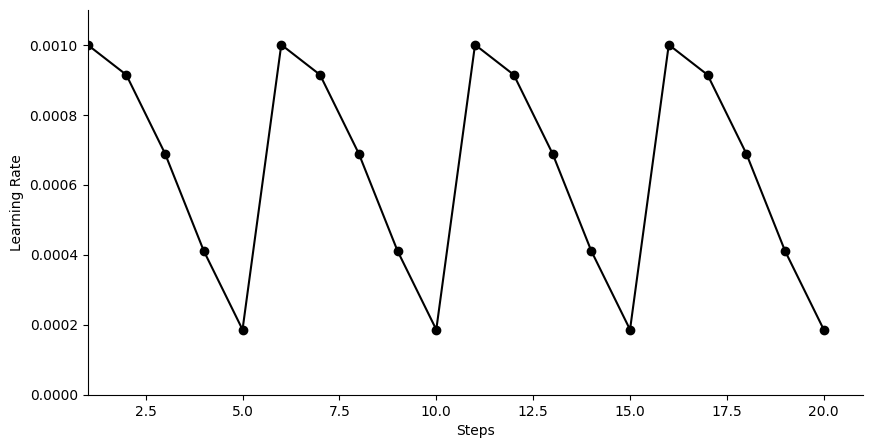
\includegraphics[width=0.6\textwidth]{imatges/preliminaries/cosinus-learning-rate-scheduler.png}
    \caption[Cosinus Cycling Learning]{\textit{Cosinus Cycling Learning. The graphic show how the learning rate varies following the cosinus functions over the epochs. Illustration by Author}}
    {\label{fig:cycling-rate-decay}}
    \end{figure}
\end{itemize}

\vspace{0.5cm}
\textbf{Dropout} \\

Dropout is a regularization method \cite{DropoutPaper}. The idea behind dropout is to prevent overfitting and improve generalization in neural networks by randomly "dropping out" or deactivating a fraction of the neurons during each training iteration. \\

By randomly dropping out neurons, the network becomes more robust and less sensitive to the precise configuration of any single neuron. It forces the network to learn redundant representations and prevents co-adaptation.

\begin{figure}[H]
\centering
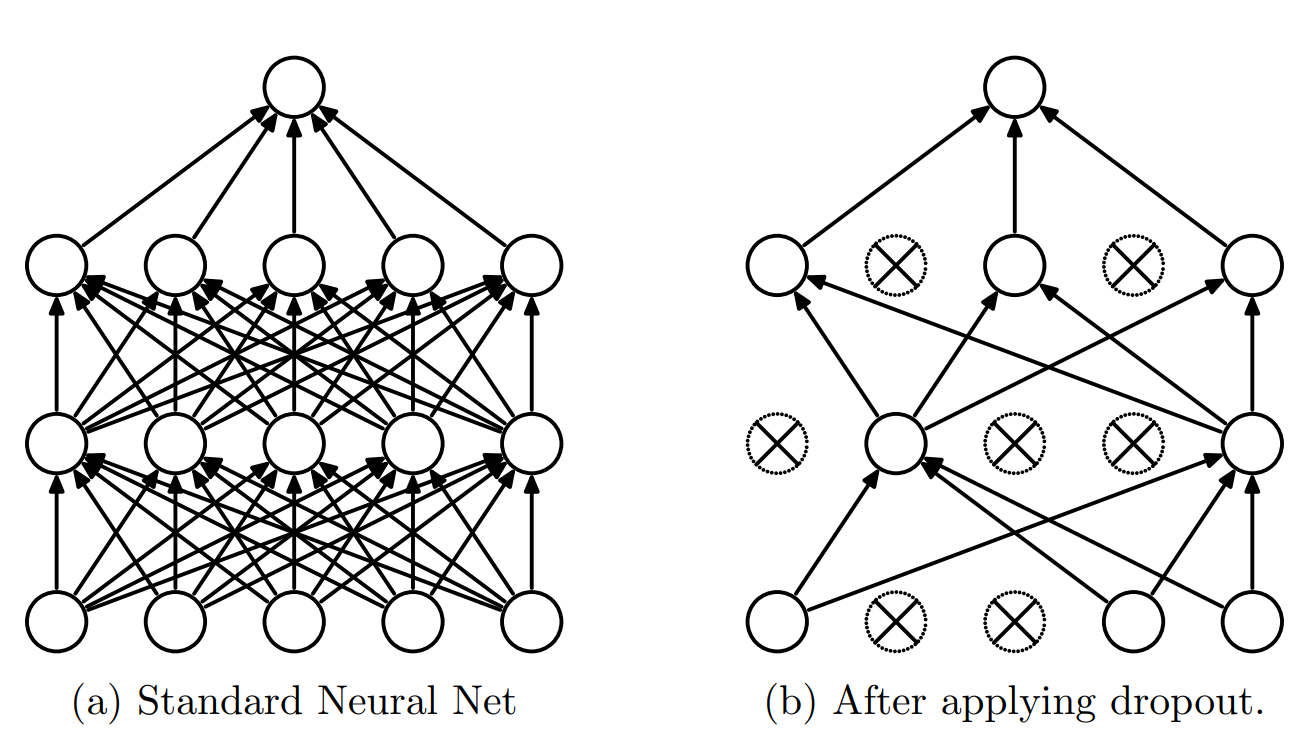
\includegraphics[width=10cm]{imatges/preliminaries/dropout.png}
\caption[Dropout]{\textit{Dropout Neural Net Model. \textbf{Left}: A standard neural net with 2 hidden layers. \textbf{Right}:
An example of a thinned net produced by applying dropout to the network on the left.
Crossed units have been dropped. Illustration by Srivastava}}
{\label{fig:dropout}}
\end{figure}

\subsection{Train, Validation and Test Sets}

The primary method employed to validate the models involves dividing the original dataset into three subsets using the Holdout set scheme, see \textit{Figure \ref{fig:holdout-test-scheme}}. The percentages applied to divide to the ISIC dataset used for training is 80\%, for validation 10\% and for testing 10\%. \\

Bellow there are the explanation of each dataset and the propose of all of them. \\

\vspace{0.5cm}
\textbf{Training Set} \\

This subset is utilized during the training phase of the model. \\

\vspace{0.5cm}
\textbf{Validation Set} \\

This subset was employed to apply trained models to new, unseen examples and evaluate the model's performance. It also aids in selecting the model that best matches the validation set by minimizing the classifier One vs Rest metric in predictions. \\

\vspace{0.5cm}
\textbf{Test Set} \\

Comprising non-observed data examples, this set is used to assess the performance of the chosen model. It helps determine if further optimization is required and which techniques should be applied next. Alternatively, it aids in deciding whether to select an alternative model.


\begin{figure}[H]
\centering
\includegraphics[width=0.8\textwidth]{imatges/preliminaries/train-test-validation-sets.png}
\caption[Holdout Test Scheme]{\textit{Holdout Test Scheme. Illustration by Qualcomm}}
{\label{fig:holdout-test-scheme}}
\end{figure}

\newpage

\subsection{Data Augmentation}

Data augmentation encompasses various techniques utilized to expand the dataset by introducing modifications, thereby increasing the number of examples. Its purpose is not only to enlarge the dataset but also to enhance its diversity. By acting as a regularizer, data augmentation aids in mitigating overfitting during machine learning model training.

\begin{figure}[H]
\centering
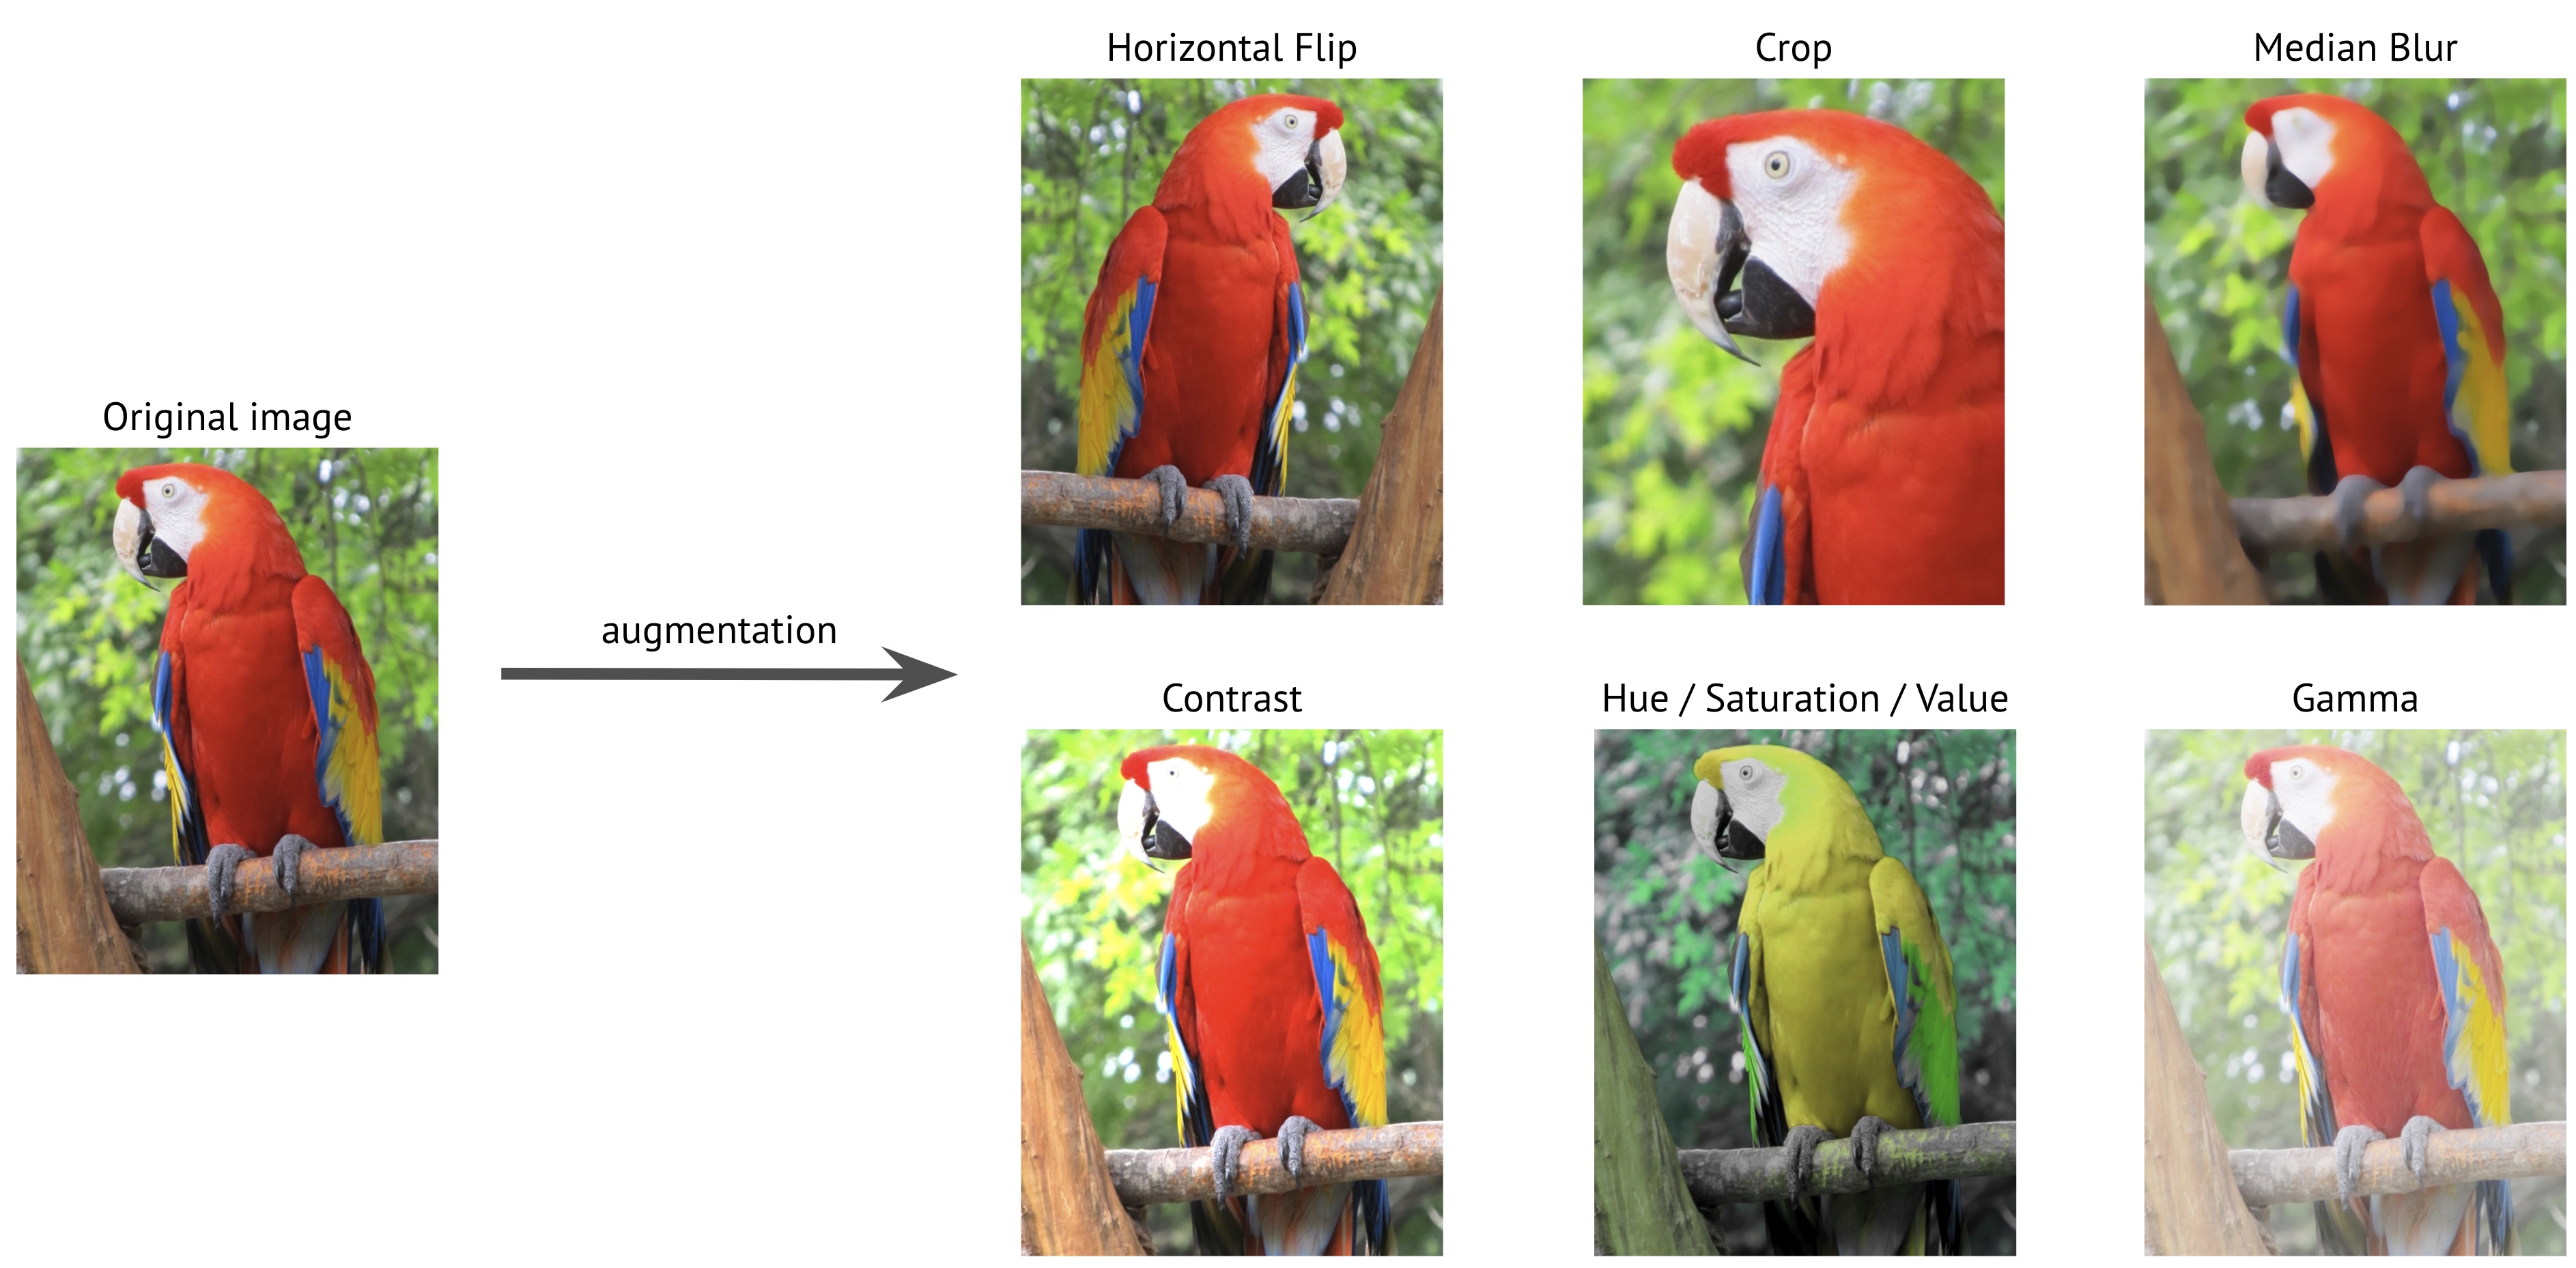
\includegraphics[width=0.7\textwidth]{imatges/preliminaries/augmentation.jpg}
\caption[Data Augmentation]{\textit{Data Augmentation. The example show the result of applying some transformation to an image. Illustration by Albumentations}}
{\label{fig:augmentation}}
\end{figure}


\subsection{Test-Time Augmentation}

Test-time augmentation (TTA) is used during the testing or inference phase of a machine learning model. TTA generates multiple augmented versions of test samples to obtain diverse predictions. By obtaining predictions from these augmented samples and combining them, TTA mimics the behavior of an ensemble of models.

\begin{figure}[H]
\centering
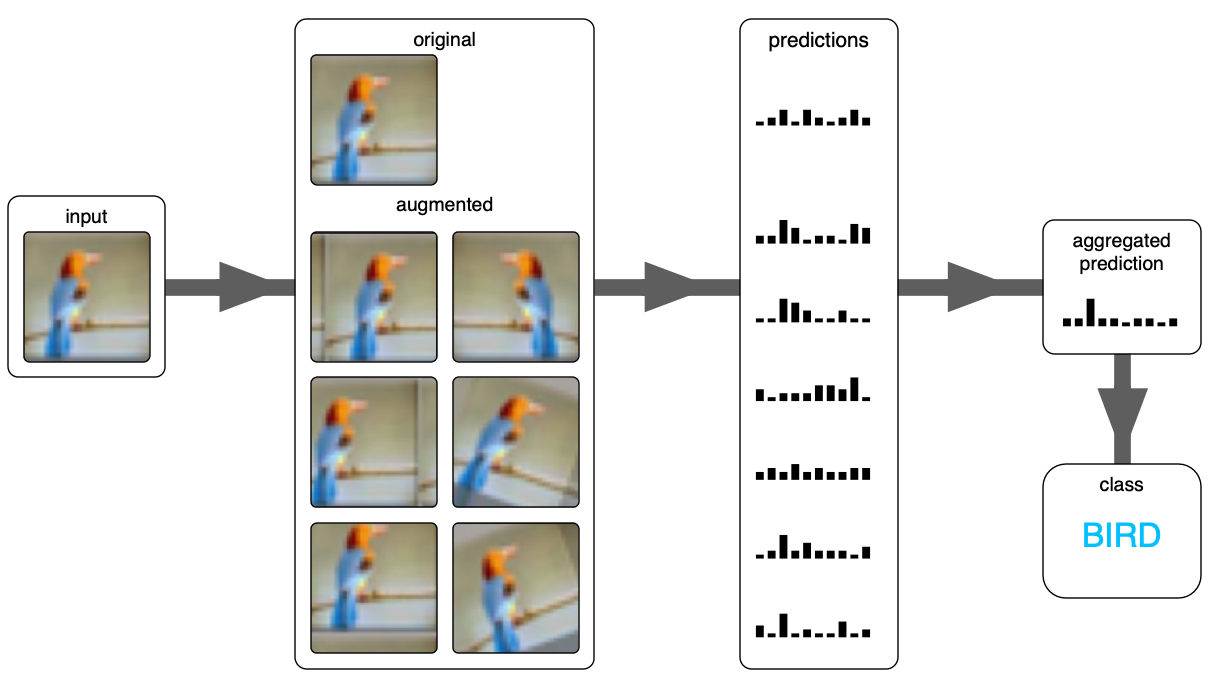
\includegraphics[width=0.8\textwidth]{imatges/preliminaries/tta.png}
\caption[Test-Time Augmentation]{\textit{Test-Time Augmentation. Illustration by stepup.ai}}
{\label{fig:tta}}
\end{figure}

\newpage

\subsection{ResNet}

ResNet, short for "Residual Network," is a deep convolutional neural network (CNN) architecture that was introduced in 2015 by researchers from Microsoft Research \cite{ResNetPaper}. It revolutionized the field of deep learning by addressing the challenge of training very deep neural networks. \\

The main problem encountered when training deep neural networks is the degradation problem, where the accuracy of the model saturates and then starts to decline rapidly as the network depth increases. This degradation occurs due to the difficulty of optimizing the network's parameters and the vanishing gradient problem, where gradients become extremely small during backpropagation, making it difficult for the network to learn effectively. \\

ResNet tackled this problem by introducing the concept of residual learning. The key idea is to use "skip connections" or "identity mappings" that allow the network to learn residual functions. Instead of trying to learn the underlying mapping directly, ResNet models learn the residual between the desired mapping and the input. \\

By introducing these skip connections, ResNet models can effectively "skip" one or more layers during training, allowing information to flow more easily through the network. This mitigates the degradation problem and enables the training of extremely deep networks (e.g., hundreds of layers) without suffering from diminishing accuracy. \\

In ResNet, each layer of the network contains a residual block. A residual block consists of multiple convolutional layers followed by batch normalization and activation functions. The input to a residual block is added to its output through a skip connection, which directly connects the input to the output. This allows the network to learn the residual information, or the difference between the input and the desired output, making it easier for the network to learn the underlying mapping.  \\

There are various architectural variants or "flavors" of ResNet, including {\tt ResNet-152}, {\tt ResNet-101}, {\tt ResNet-50}, {\tt ResNet-34}, and {\tt ResNet-18}. The number following the name of each ResNet variant indicates the number of inner layers present in the architecture.

\newpage

As evident from \textit{Figure \ref{fig:resnet}}, it can be observed that ResNet architectures with a greater number of layers tend to exhibit higher accuracy. However, it is important to note that this improvement in accuracy comes at the expense of having a significantly larger number of parameters to train.


\begin{figure}[H]
\begin{adjustbox}{width=\textwidth, trim={0pt 0pt 1cm 0pt}, clip}
\centering
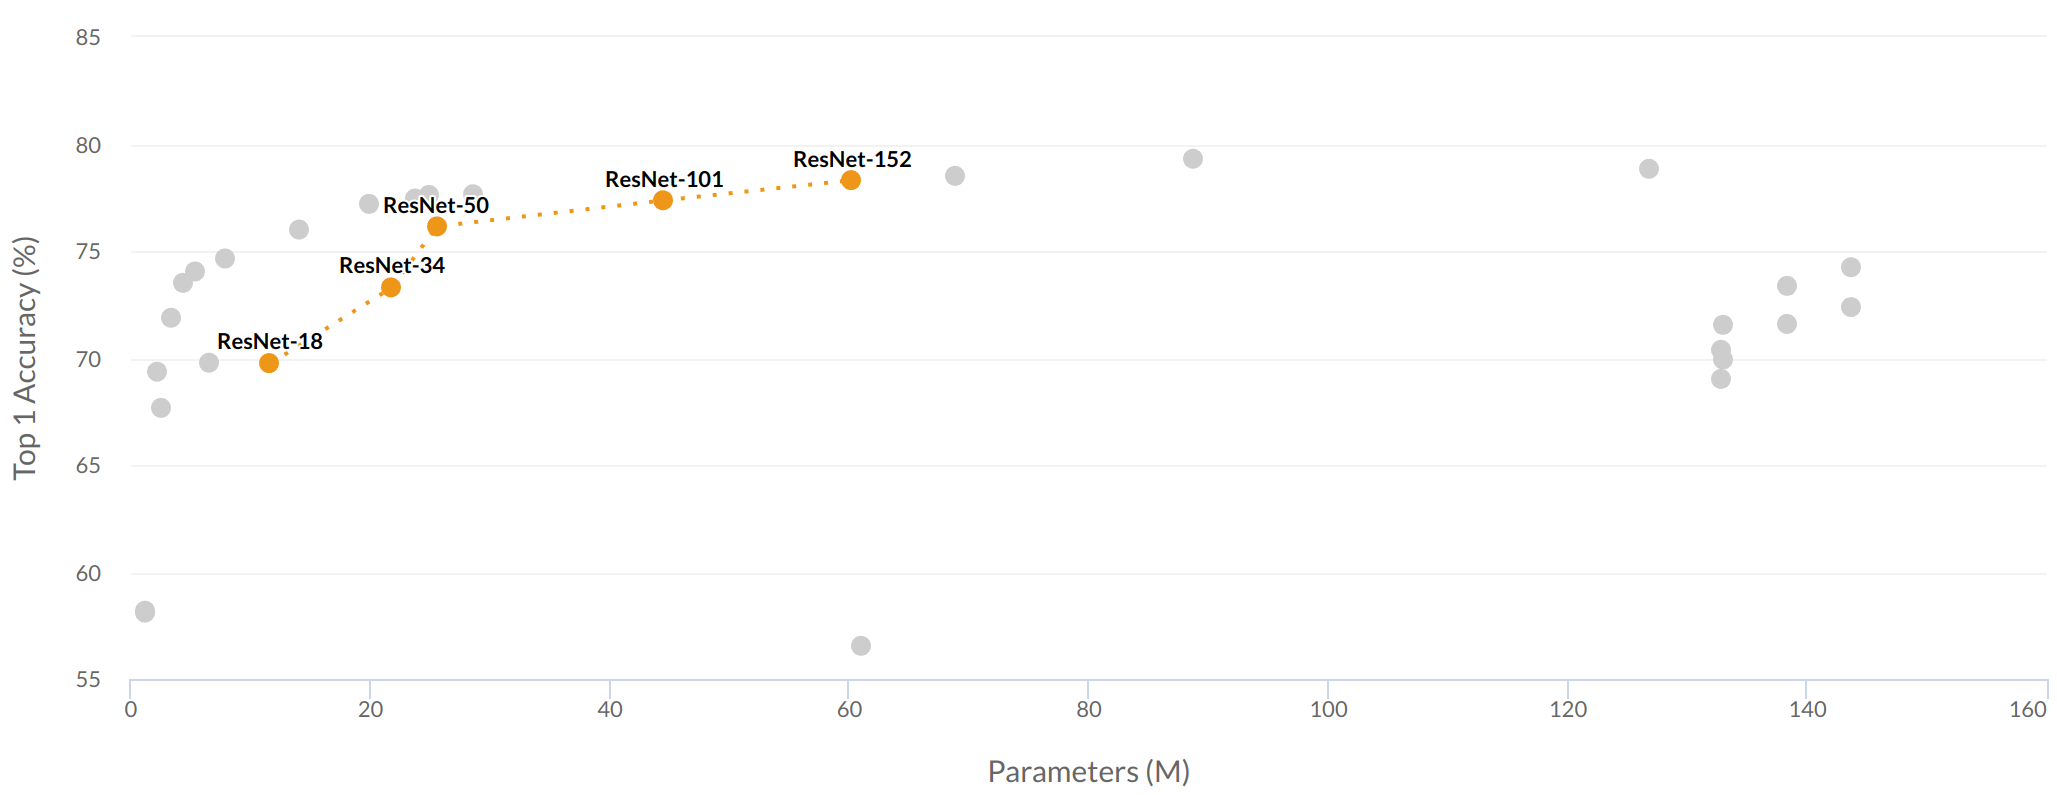
\includegraphics[width=\textwidth]{imatges/preliminaries/ResNetImageNet.png}
\end{adjustbox}
\caption[ResNet "flavors" Results on ImageNet]{\textit{ResNet "flavors" Results on ImageNet. Illustration by paperswithcode}}
{\label{fig:resnet}}
\end{figure}

To accurately assess the performance of each ResNet architecture, refer to the \textit{Table \ref{table:resnet}}, which provides the accuracy achieved on the ImageNet dataset along with the corresponding number of trainable parameters in millions.

\begin{table}[H]
\centering
\begin{tabular}{lcc}
\toprule
\textbf{Model} & \textbf{Accuracy} & \textbf{Parameters} \\
 \midrule
ResNet-152 & 78.31\% & 60.2M \\
ResNet-101 & 77.37\% & 44.5M \\
ResNet-50 & 76.15\% & 25.6M \\
ResNet-34 & 73.30\% & 21.8M \\
ResNet-18 & 69.76\% & 11.7M \\ \bottomrule
\end{tabular}
\caption[Accuracy Achieved on ImageNet and Trainable Parameters of Each ResNet.]
 {\textit{Accuracy Achieved on ImageNet and Trainable Parameters of Each ResNet.
  Each image in the ImageNet dataset is associated with 1 of 1,000 classes. Table by paperswithcode}}
{\label{table:resnet}}
\end{table}

\newpage

\section{Technical Background}

This section provides an introduction to the technical concepts
that surround the creation of the CAD system, such as microservices architecture, model exposing, code packaging, containerization, platform deployment.

\subsection{Microservices Architecture}

A microservices architecture is a software design approach that structures an application as a collection of small, independent services, each running in its own process and communicating with each other through lightweight mechanisms. This architecture promotes scalability, modularity, and flexibility. \\

The present thesis consists of two services: an API and a UI. These services are built using different frameworks and programming languages.


\subsection{Inference API}

The inference API service focuses on handling the back-end logic and data processing. It exposes a well-defined API that allows user to interact with the trained models. \\

The main end-points that the present thesis API service exposes are explained bellow. The completed source code is not given here, but it can be found in the GitHub repository or in the source code attached to the the thesis. \\

\vspace{0.5cm}
\textbf{Consulting Available Models} \\

This end-point returns the list of the available models configured in the configuration file of the API.

\begin{Verbatim}[fontsize=\small]
@app.get("/public_models")
async def public_models():
    """
    Description
    ----------
    Returns the name of the available models
    """
    ...
\end{Verbatim}


\vspace{0.5cm}
\textbf{Predict a Single Image} \\

This end-point captures an image and a model identifier creating a unique task and makes the prediction just in time.

\begin{Verbatim}[fontsize=\small]
@app.post("/predict")
async def predict(file: UploadFile = File(...),
                    model_id='vicorobot.8c_b3_768_512_18ep_best_fold0'):
    """
    Description
    ----------
    The function receives a file (expected img with jpeg format)
    then it creates the task that is being returned
    and async does the prediction.
    """
    ...
\end{Verbatim}

\vspace{0.5cm}
\textbf{Predict a Jar of Images} \\

This endpoint behaves similarly to the previous endpoint, with the key difference being that it supports predicting a set of images instead of just one. Additionally, the predictions of the images are made in a separate thread, preventing the system from getting stuck due to the time it would take to predict a large number of images.

\begin{Verbatim}[fontsize=\small]
@app.post("/predict_bulk")
async def predict_bulk(bg_tasks: BackgroundTasks,
                       files,
                       model_id='vicorobot.8c_b3_768_512_18ep_best_fold0'):
    """
    Description
    ----------
    Recives a jar of images and then it creates a task
    for this predict that is returned to consult the result
    of the predictions of each img.

    Returns
    -------
    task_id: str
        - folder where the images where saved
    num_files: int
        - number of images saved
    """
    ...
\end{Verbatim}

\vspace{0.5cm}
\textbf{Consult the Predictions} \\

When an inference is made, users need a way to access the results of the requested prediction. To handle this, the inference process stores the predictions and metadata of the models in CSV files within the task directory. These CSV files are then retrieved and combined to generate a response for the client.

\begin{Verbatim}[fontsize=\small]
@app.get("/from_task/{task_id}")
async def from_task(task_id: str):
    """
    Description
    ----------
    Consults the predictions from a task
    """
    ...
\end{Verbatim}

\newpage

\vspace{0.5cm}
\textbf{Exposing the Models} \\

The concept of handling long-running tasks in the background is often implemented to improve the responsiveness and scalability of the system. This approach allows the client to initiate a task and receive a unique identifier, which can later be used to query or retrieve the results of that task (\textit{Figure \ref{fig:backgrond-task}}). \\


\begin{figure}[H]
\centering
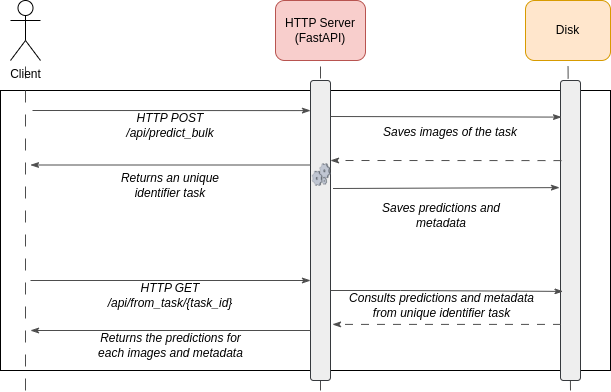
\includegraphics[width=0.9\textwidth]{imatges/preliminaries/BackgroundTask.drawio.png}
\caption[Inferring Images Through the Background Task Mechanism]{\textit{Inferring Images Through the Background Task Mechanism. Notice that in this way we avoid to congest the API thread. Illustration by Author}}
{\label{fig:backgrond-task}}
\end{figure}

When an HTTP task is required, it comes with the identifier of the model that will be used to infer the image or a jar of images. This model is searched for in a volume configuration file located in the API. The configuration file must contain the entry for the model identifier and also include the path to the binary trained model. The trained model is deserialized and used at runtime through the PyTorch API. \\

Once the path of the model in the operating system is obtained it is as easy as load the searilized model
using the PyTorch API as follow:

\begin{Verbatim}[fontsize=\small]
instance_nn = class_nn(out_dim)
checkpoint = torch.load(pytorch_model_path, map_location=device)
model_state_dict = checkpoint['model_state_dict']
instance_nn.load_state_dict(model_state_dict, strict=True)
\end{Verbatim}

\subsection{Containerization}

Containerization is a technology that allows applications and their dependencies to be packaged into isolated, lightweight containers. These containers provide an encapsulated runtime environment, ensuring that the application runs consistently across different systems. \\

Containers are created from container images, which are self-contained packages containing the application's code, dependencies, libraries, and configurations. Images serve as the blueprint for creating containers. They can be shared, versioned, and easily deployed on various platforms. \\

Virtualization frameworks, such as Docker and Podman, provide tools and services to build, manage, and run containers. These frameworks utilize underlying virtualization technologies to create and manage isolated environments. These environments, called containers, offer resource isolation and ensure that applications run consistently across different computing environments.

\subsection{Platform Deployment}

To distribute the containerized API and UI services easily to professionals, there are several solutions available. In this thesis, I propose the creation of a shell script that performs the following steps:

\begin{itemize}
\item Creates a directory in the system's home directory to download the source code and artifacts.
\item Clones the source code repository from GitHub.
\item Moves the encapsulated Python packages into the API source code.
\item Builds the API image.
\item Builds the UI image.
\item Clones the artifacts from GitLab.
\item Activates the services using a Docker Compose file, which starts the containers with their configurations based on the previously built images.\end{itemize}


By following this approach, professionals can easily distribute the containerized services by running the provided shell script.


\chapter{Studies and Decisions}
\label{cap:studies_and_decisions}

This chapter is dedicated to exploring the essential tools required for the project's development and understanding their significance. The initial section of this chapter focuses on delineating the functional and non-functional requirements that the system must fulfill. Subsequently, the second part identifies and elucidates the selected technologies for the project.

\section{System Requirement}

This section explores the necessary requirements for detecting melanoma. It is important to distinguish between the final system and the work involved in its development. Constructing and training a Convolutional Neural Network (CNN) requires substantial computational power, sophisticated libraries, and often a significant amount of time. However, once the model has been trained and saved, it can be readily used. Typically, the response time inferring is within seconds. Yet the inference time of the models is few we also need to take into account the time wasted in the HTTP request and the time wasted in showing the results. \\

The requirements can be classified into two categories:

\begin{itemize}
    \item \textbf{Functional requirements}

    Functional requirements pertain to the capabilities that the product must possess to fulfill specific user needs.

    \item \textbf{Non-functional requirements}

    Non-functional requirements encompass aspects such as usability, performance, reliability.
\end{itemize}

\newpage

\vspace{0.5cm}
\textbf{Functional requirements} \\

The functional requirements of the system are:

\begin{itemize}
    \item The objective is to classify whether a single image or a set of images, specifically from a dermoscopy, contains a melanoma or not. The classification task is binary, aiming to determine the presence or absence of melanoma.

    \item Expose models through an API that can classify whether an image or a set of images contains melanoma or not. The API should not only provide the classification results but also offer additional information such as the specific model used and the probabilities associated with the prediction..

    \item A user-friendly interface (UI) is implemented to facilitate loading of images and communicate with the API via the HTTP protocol for image inference. The UI should display the results of the selected model for the bulk of loaded images.

    \item Create images of each service, to distribute the services using container technology.
\end{itemize}

\vspace{0.5cm}
\textbf{Non-functional requirements} \\

For training models, Jupyter Notebook, Python3, and Anaconda are used, ensuring compatibility with any computer to run the code and classify images. Sufficient RAM is required to handle the desired images effectively. \\

Since the API and UI services are containerized, any container management tool such as Docker or Podman can be used, providing the necessary environment to work with containers.

\newpage

\section{Hardware}

The hardware used for the thesis encompassed a range of machines. The primary development machine employed was a laptop with limited performance. Additionally, a machine provided by Google was utilized within the Google Colab environment for training models that did not require high computational capabilities. Furthermore, for a week of work at the VICOROB laboratory, a separate machine was utilized specifically for training models with more extensive data augmentation requirements, necessitating higher computational resources. \\

\textit{Table \ref{table:dev-machine}, \ref{table:google-machine}, and \ref{table:vicorobot-machine}} provide an overview of the characteristics of the machines employed for the project. Each of these machines had its own specific use, and it is recommended to select the an appropriate machine based on specific needs.

\begin{table}[H]
	\centering
	\begin{tabular}{cc}
		\toprule
		\multicolumn{2}{c}{\textbf{Development Machine}} \\
		\midrule
		OS & Fedora Linux 38 \\
		CPU & Intel i5-8250U \\
		GPU & Intel UHD Graphics 620 \\
		RAM & 8GB \\
		Disk & 225GB \\
		\bottomrule
	\end{tabular}
  \caption[Development Machine Metrics.]
  {\textit{Development Machine Metrics.
  This machine was only used for programming and searching thesis information.
  Table by Author}}
	\label{table:dev-machine}
\end{table}


\begin{table}[H]
	\centering
	\begin{tabular}{cc}
			\toprule
			  \multicolumn{2}{c}{\textbf{Google Machine}} \\
			  \midrule
			  OS & Ubuntu 20.04.6 LTS \\
			  CPU & Intel Xeon \\
			  GPU & Tesla T4, 16GB \\
			  RAM & 12GB \\
			  Disk & 125GB \\
			  \bottomrule
\end{tabular}
\caption[Google Machine Metrics.]
  {\textit{Google Machine Metrics.
  Note that this machine was used to train models that take at most a pair of hours to accomplish the training.
  Table by Author}}
{\label{table:google-machine}}
\end{table}

\newpage

\begin{table}[H]
\centering
\begin{tabular}{cc}
	 \toprule
		\multicolumn{2}{c}{\textbf{VICOROB Machine}} \\
		\midrule
		OS & Ubuntu 20.04.2 LTS \\
		CPU & Intel(R) Xeon(R) Silver \\
		GPU & A100, 80GB\\
		RAM & 396GB \\
		Disk & 6.3T \\
		\bottomrule
\end{tabular}
\caption[VICOROB Machine Metrics.]
  {\textit{VICOROB Machine Metrics.
  This machine was used to train models that required high computational resources because of data augmentation.
  Table by Author}}
{\label{table:vicorobot-machine}}
\end{table}

\section{Software}

In order to establish and operate the CAD infrastructure, it was crucial to establish separate environments for creating the services and training the models, ensuring that all the required packages were included. The detailed instructions for setting up these distinct environments can be found in \textit{Appendix \ref{appendix:appendix_a}}. Additionally, \textit{Appendix \ref{appendix:appendix_b}} provides a guide on deploying and activating the services within the CAD infrastructure. \\

The following pages will outline and provide detailed descriptions of each tool utilized throughout the thesis. These tools played a crucial role in various aspects, including the training process, creation of services such as user interface (UI) and application programming interface (API), deployment of these services with trained models, management of the source code, and comprehensive documentation. Each tool's significance and contribution to the thesis will be thoroughly explained, shedding light on their specific functionalities and importance in the research project.

\newpage

\vspace{0.5cm}
\textbf{Python 3.9} \\

Python (\textit{Figure \ref{fig:python-logo}}) is a high-level, interpreted programming language known for its simplicity and readability. It was created by Guido van Rossum and released in 1991. Its design philosophy emphasizes code readability with the use of significant indentation. \\

Python is an ideal choice for machine learning and AI-based projects due to several advantages. These include its simplicity and consistency, access to excellent libraries and frameworks specifically designed for AI and ML, flexibility, platform independence, and a large and supportive community.

\begin{figure}[H]
\centering

\includegraphics[width=0.15\textwidth]{imatges/studies_and_decisions/python-logo-only.png}
\caption[Python Logo]{\textit{Python Logo. Illustration by Python Software Foundation}}
{\label{fig:python-logo}}
\end{figure}

\vspace{0.5cm}
\textbf{Anaconda} \\

Anaconda (\textit{Figure \ref{fig:anaconda-logo}}) is a widely used open-source distribution of the Python programming language. It simplifies the management and deployment of data science and machine learning environments. With Anaconda, you can easily install and manage Python packages using the conda package management system. It also provides tools for creating isolated environments to ensure consistent dependencies and package versions.

\begin{figure}[H]
\centering
  \begin{adjustbox}{trim=0cm 1cm 0cm 1cm, clip}

\includegraphics[width=0.5\textwidth]{imatges/studies_and_decisions/anaconda-logo.png}
\end{adjustbox}
\caption[Anaconda Logo]{\textit{Anaconda Logo. Illustration by Anaconda}}
{\label{fig:anaconda-logo}}
\end{figure}


\vspace{0.5cm}
\textbf{Jupyter Notebook} \\

Jupyter Notebook (\textit{Figure \ref{fig:jupyter-logo}}) is an open-source web application that allows to create and share interactive documents containing live code, visualizations, and text. It provides an environment for data analysis, visualization, and prototyping. With Jupyter Notebooks, you can write and execute code in individual cells, making it easy to experiment and iterate. It supports multiple programming languages such as Python, R and Haskell.

\begin{figure}[H]
\centering

\includegraphics[width=0.2\textwidth]{imatges/studies_and_decisions/jupyter-notebook.png}
\caption[Jupyter Notebook Logo]{\textit{Jupyter Notebook Logo. Illustration by Jupyter.org}}
{\label{fig:jupyter-logo}}
\end{figure}

\vspace{0.5cm}
\textbf{CUDA} \\

CUDA (\textit{Figure \ref{fig:cuda-logo}}), which stands for Compute Unified Device Architecture, is a parallel computing platform and programming model developed by NVIDIA. It enables developers to leverage the power of NVIDIA GPUs (Graphics Processing Units) for high-performance computing tasks. \\

CUDA has gained widespread adoption in the scientific and computational research communities due to its ability to leverage the computational power of GPUs. It has become an essential tool for accelerating a wide range of applications, from physics simulations and computational biology to data analytics and artificial intelligence.

\begin{figure}[H]
\centering
\begin{adjustbox}{trim=0cm 0.25cm 0cm 0.5cm, clip}

\includegraphics[width=0.325\textwidth]{imatges/studies_and_decisions/nvidia-cuda.jpg}
\end{adjustbox}
\caption[CUDA Logo]{\textit{CUDA Logo. Illustration by Nvidia Corporation}}
{\label{fig:cuda-logo}}
\end{figure}

\vspace{0.5cm}
\textbf{PyTorch} \\

PyTorch (\textit{Figure \ref{fig:pytorch-logo}}) is an open-source machine learning framework widely used for deep learning tasks. It provides a flexible and dynamic approach to building and training neural networks. PyTorch stands out for its integration of GPU acceleration, enabling efficient computations using NVIDIA GPUs. \\

PyTorch offers a high-level API called torchvision, which simplifies common computer vision tasks such as image classification, object detection, and image generation. It also integrates with other libraries and tools in the Python ecosystem, making it easy to combine PyTorch with popular frameworks like NumPy, SciPy, and pandas.

\begin{figure}[H]
\centering

\includegraphics[width=0.325\textwidth]{imatges/studies_and_decisions/pytorch-logo.png}
\caption[PyTorch Logo]{\textit{PyTorch Logo. Illustration by PyTorch.org}}
{\label{fig:pytorch-logo}}
\end{figure}

\vspace{0.5cm}
\textbf{OpenCV} \\

OpenCV (Open Source Computer Vision Library), is a popular open-source computer vision and image processing library. It provides a wide range of functions and algorithms for tasks such as image and video processing, object detection and tracking, feature extraction, and more. \\

OpenCV (\textit{Figure \ref{fig:opencv-logo}}) allows developers to read, write, and manipulate images and videos efficiently. The library offers various image processing functions, including filtering, resizing, color conversion, and geometric transformations.

\begin{figure}[H]
\centering
\begin{adjustbox}{trim=1cm 1cm 1cm 1cm, clip}

\includegraphics[width=0.7\textwidth]{imatges/studies_and_decisions/OpenCV-logo.png}
\end{adjustbox}
\caption[OpenCV Logo]{\textit{OpenCV Logo. Illustration by OpenCV Team}}
{\label{fig:opencv-logo}}
\end{figure}


\vspace{0.5cm}
\textbf{Albumentations} \\

Albumentations (\textit{Figure \ref{fig:albumentations-logo}}) is an open-source Python library for image augmentation in machine learning and computer vision tasks. It provides a wide range of transformations and optimizations to enhance training data, improving the performance and generalization of machine learning models. With high-performance implementation and seamless integration with popular frameworks, Albumentations is widely used for efficient and customizable image augmentation.

\begin{figure}[H]
\centering

\includegraphics[width=0.13\textwidth]{imatges/studies_and_decisions/albumentations-logo.png}
\caption[Albumentations Logo]{\textit{Albumentations Logo. Illustration by Albumentations Team}}
{\label{fig:albumentations-logo}}
\end{figure}


\vspace{0.5cm}
\textbf{NumPy} \\

NumPy (\textit{Figure \ref{fig:numpy-logo}}) is a Python library for efficient numerical computing. It provides a powerful array object for manipulation and computation of multidimensional arrays. With optimized operations and support for broadcasting.

\begin{figure}[H]
\centering

\includegraphics[width=0.225\textwidth]{imatges/studies_and_decisions/numpy-logo.png}
\caption[NumPy Logo]{\textit{NumPy Logo. Illustration by NumPy Organazation}}
{\label{fig:numpy-logo}}
\end{figure}


\vspace{0.5cm}
\textbf{Pandas} \\

Pandas (\textit{Figure \ref{fig:pandas-logo}}) is a popular Python library for data manipulation and analysis. It provides data structures and functions to efficiently work with structured data, such as tabular data and time series. Pandas' key features include its DataFrame object, which allows for easy handling of data, indexing, filtering, and aggregation operations. With its intuitive and powerful functionality, Pandas is widely used in data preprocessing, exploration, and analysis tasks.

\begin{figure}[H]
\centering

\includegraphics[width=0.3\textwidth]{imatges/studies_and_decisions/pandas-logo.png}
\caption[Pandas Logo]{\textit{Pandas Logo. Illustration by The pandas development team}}
{\label{fig:pandas-logo}}
\end{figure}


\vspace{0.5cm}
\textbf{Matplotlib} \\

Matplotlib (\textit{Figure \ref{fig:matplotlib-logo}}) is a widely-used Python library for creating static, animated, and interactive visualizations. It provides a flexible and comprehensive range of functions and tools for generating plots, charts, histograms, and more. Matplotlib allows customization of various aspects of visualizations, including colors, labels, titles, axes, and legends. With its extensive functionality and compatibility with NumPy arrays, Matplotlib is a go-to library for data visualization and presentation in Python.

\begin{figure}[H]
\centering

\includegraphics[width=0.45\textwidth]{imatges/studies_and_decisions/matplotlib-logo.png}
\caption[Matplotlib Logo]{\textit{Matplotlib Logo. Illustration by Matplotlib Organization}}
{\label{fig:matplotlib-logo}}
\end{figure}

\vspace{0.5cm}
\textbf{Seaborn} \\

Seaborn (\textit{Figure \ref{fig:seaborn-logo}}) is a Python data visualization library built on top of Matplotlib. It provides a high-level interface for creating attractive and informative statistical graphics. Seaborn simplifies the process of generating complex visualizations by offering a range of built-in functions for creating appealing plots, such as scatter plots, histograms, bar plots, and heatmaps. Seaborn is widely used for exploratory data analysis and presentation of statistical insights.

\begin{figure}[H]
\centering
\includegraphics[width=0.25\textwidth]{imatges/studies_and_decisions/seaborn-logo.png}
\caption[Seaborn Logo]{\textit{Seaborn Logo. Illustration by Seaborn Organization}}
{\label{fig:seaborn-logo}}
\end{figure}

\vspace{0.5cm}
\textbf{WandB} \\

Weights \& Biases (\textit{Figure \ref{fig:wandb-logo}}) is a machine learning experiment tracking and visualization platform. It offers a suite of tools to track, organize, and analyze machine learning experiments. With wandb, developers can log metrics, hyperparameters, and model checkpoints during training, making it easy to compare and analyze different experiments.

\begin{figure}[H]
\centering
\includegraphics[width=0.4\textwidth]{imatges/studies_and_decisions/wandb-logo.png}
\caption[Seaborn Logo]{\textit{Seaborn Logo. Illustration by Weights \& Biases Inc}}
{\label{fig:wandb-logo}}
\end{figure}

\vspace{0.5cm}
\textbf{FastAPI} \\

FastAPI (\textit{Figure \ref{fig:fastapi-logo}}) is a modern, high-performance web framework for building APIs with Python. It emphasizes simplicity, speed, and type annotations to create efficient and scalable web applications. FastAPI leverages Python's type hints for automatic request and response validation, enabling faster development and reducing the chances of introducing bugs. It provides asynchronous capabilities using Python's asyncio framework, allowing for high-concurrency and efficient handling of multiple requests. With its intuitive API declaration syntax and automatic generation of interactive documentation, FastAPI simplifies the process of building robust and well-documented APIs.

\begin{figure}[H]
\centering
\begin{adjustbox}{trim=0cm 0.25cm, clip}
\includegraphics[width=0.35\textwidth]{imatges/studies_and_decisions/fastapi-logo.png}
\end{adjustbox}
\caption[FastAPI Logo]{\textit{FastAPI Logo. Illustration by tiangolo}}
{\label{fig:fastapi-logo}}
\end{figure}

\vspace{0.5cm}
\textbf{JS} \\

JavaScript (\textit{Figure \ref{fig:js-logo}}) is a versatile programming language primarily used for client-side web development. It enables dynamic and interactive functionality on websites, allowing for real-time manipulation of HTML elements, handling user events, and modifying web page content.

\begin{figure}[H]
\centering
\begin{adjustbox}{trim=0cm 0cm, clip}
\includegraphics[width=0.15\textwidth]{imatges/studies_and_decisions/js-logo.png}
\end{adjustbox}
\caption[JS Logo]{\textit{JS Logo. Illustration by JS Organization}}
{\label{fig:js-logo}}
\end{figure}

\newpage

\vspace{0.5cm}
\textbf{SvelteKit} \\

SvelteKit (\textit{Figure \ref{fig:sveltekit-logo}}) is a high-performance JavaScript framework for building web applications. It uses a compiler-based approach, resulting in optimized applications with minimal overhead. It provides built-in routing, supports Server-Side Rendering (SSR) and Static Site Generation (SSG), and promotes component reusability. SvelteKit offers a developer-friendly environment, integrates well with APIs, and generates small bundles for faster loading times.

\begin{figure}[H]
\centering
\begin{adjustbox}{trim=0cm 0cm, clip}
\includegraphics[width=0.12\textwidth]{imatges/studies_and_decisions/sveltekit-logo.png}
\end{adjustbox}
\caption[SvelteKit Logo]{\textit{SvelteKit Logo. Illustration by WIKIPEDIA}}
{\label{fig:sveltekit-logo}}
\end{figure}

\vspace{0.5cm}
\textbf{Docker} \\

Docker (\textit{Figure \ref{fig:docker-logo}}) is an open-source platform for building and deploying applications in isolated containers. It simplifies application management, ensures portability across different environments, and provides isolation for enhanced scalability and security. With Docker, developers can package applications and their dependencies into lightweight, self-contained containers, making deployment and scaling more efficient.

\begin{figure}[H]
\centering
\begin{adjustbox}{trim=0cm 0cm, clip}
\includegraphics[width=0.4\textwidth]{imatges/studies_and_decisions/docker-logo.png}
\end{adjustbox}
\caption[SvelteKit Logo]{\textit{SvelteKit Logo. Illustration by WIKIPEDIA}}
{\label{fig:docker-logo}}
\end{figure}


\vspace{0.5cm}
\textbf{Podman} \\

Podman (\textit{Figure \ref{fig:podman-logo}}) is designed to manage containers and container images, offering features similar to Docker but with a focus on security and compatibility with industry standards. It allows you to build, run, and manage containers without the need for a separate daemon. \\

One key advantage of Podman is its rootless mode, which allows users to run containers as non-root, enhancing security and isolation. This eliminates the need for privileged access, making Podman a preferred choice for environments where running containers as non-root is required.

\begin{figure}[H]
\centering
\begin{adjustbox}{trim=0cm 0.25cm, clip}
\includegraphics[width=0.3\textwidth]{imatges/studies_and_decisions/podman-logo.png}
\end{adjustbox}
\caption[Podman Logo]{\textit{Podman Logo. Illustration by Red Hat}}
{\label{fig:podman-logo}}
\end{figure}

\vspace{0.5cm}
\textbf{Git} \\

Git (\textit{Figure \ref{fig:git-logo}}) is a distributed version control system used for tracking changes in software projects. It enables collaboration, allows for branching and merging, handles large projects efficiently, and provides robust backup options.

\begin{figure}[H]
\centering
\begin{adjustbox}{trim=0cm 0.25cm, clip}
\includegraphics[width=0.25\textwidth]{imatges/studies_and_decisions/git-logo.jpg}
\end{adjustbox}
\caption[Git Logo]{\textit{Git Logo. Illustration by Red Hat}}
{\label{fig:git-logo}}
\end{figure}

\vspace{0.5cm}
\textbf{GitHub \& GitLab} \\

Both GitHub (\textit{Figure \ref{fig:github-logo}}) and GitLab (\textit{Figure \ref{fig:gitlab-logo}}) serve as centralized platforms for hosting and managing Git repositories.

\begin{figure}[H]
\centering
\begin{adjustbox}{trim=0cm 0cm, clip}
\includegraphics[width=0.15\textwidth]{imatges/studies_and_decisions/github-mark.png}
\end{adjustbox}
\caption[GitHub Logo]{\textit{GitHub Logo. Illustration by GitHub}}
{\label{fig:github-logo}}
\end{figure}

\begin{figure}[H]
\centering
\begin{adjustbox}{trim=0cm 0cm, clip}
\includegraphics[width=0.15\textwidth]{imatges/studies_and_decisions/gitlab-logo.png}
\end{adjustbox}
\caption[GitLab Logo]{\textit{GitLab Logo. Illustration by GitLab}}
{\label{fig:gitlab-logo}}
\end{figure}

\vspace{0.5cm}
\textbf{LaTeX} \\

LaTeX (\textit{Figure \ref{fig:latex-logo}}) is a typesetting system used for creating high-quality documents, particularly those with mathematical equations and scientific content. It focuses on the structure and formatting of documents, allowing users to concentrate on content.

\begin{figure}[H]
\centering
\begin{adjustbox}{trim=0cm 0cm, clip}
\includegraphics[width=0.25\textwidth]{imatges/studies_and_decisions/latex-logo.png}
\end{adjustbox}
\caption[LaTeX Logo]{\textit{LaTeX Logo. Illustration by LaTeX}}
{\label{fig:latex-logo}}
\end{figure}


\chapter{Planning and Methodology}
\label{cap:plan}

\section{Feasibility Study}

Before initiating any project, it is of utmost importance to conduct a comprehensive analysis of relevant factors to gauge the likelihood of accomplishing successful outcomes. While estimating the complexity associated with developing, deploying, and maintaining machine learning (ML) systems is indeed a challenging task, it is essential to recognize that this project encompasses not only the research aspect but also significant software and infrastructure development. \\

This project requires a careful balancing act, as it involves dedicating efforts to both the research and practical implementation aspects. The development of robust software and infrastructure is crucial to support the successful integration of the deep learning models and ensure their efficient deployment and maintenance. This integration can be intricate and demanding, as it requires a deep understanding of both the ML algorithms and the software engineering principles. \\

In light of these additional dimensions, the study not only aims to evaluate the feasibility of utilizing deep learning techniques but also strives to address the complexities inherent in developing a well-rounded solution. Furthermore, the evaluation will consider the available data and resources to assess the potential of achieving satisfactory results.

\section{Technical Study}

The journey begins with research,
a dynamic element that evolves and gains strength through continuous investigation.
While it is impossible to guarantee the achievement of all objectives, the way we see it,
there are three fundamental pillars that must be addressed in advance. \\

\vspace{0.5cm}
\textbf{Defining the Use Case} \\

\textit{A perfect use case outlines a project that is precisely defined, quantifiable, attainable, and possesses clearly identified users and value.} \\

Academic researchers may find satisfaction in uncovering effective solutions that contribute to publications
and secure additional funding. Yet, this thesis aims to ensure the successful implementation of a Computer-Aided Diagnosis (CAD)
infrastructure specifically designed for classifying melanoma,
with the intention of deploying it in real-world scenarios we needed to look further than just the pure research. \\

\vspace{0.5cm}
\textbf{Equipment and Technical Knowledge} \\

Equipment and technical knowledge are interdependent and collectively contribute to the success of a machine learning project. \\

In a deep learning project, both the availability of suitable equipment and technical knowledge are essential. The correct equipment, including high performance computing resources and data collection devices, facilitates efficient data handling, prepossessing, model training, and deployment. Simultaneously, technical knowledge plays a vital role in effectively leveraging the available equipment. Understanding diverse machine learning algorithms and methodologies assists in selecting the most appropriate approaches for the problem at hand. Additionally, it is crucial to acknowledge the knowledge required to create other services that accompany the project. \\

\vspace{0.5cm}
\textbf{Importance of the Dataset} \\

The success of a project like this one depends not only on the quantity but also on the quality of the data. Data is essential for any deep learning model to learn effectively. Therefore, it is vital to invest time in
acquiring an optimal image data-set that possesses sufficient data volume, annotation, truth, and reusability. \\

For computer-based image recognition and analysis, high-quality data is necessary. The objective is to gather data from various patient populations to ensure that the data-set is diverse and accurately represents different disease states and outcomes. Often, healthcare organizations engage medical experts to review and label the data to prevent inaccurate labels and ensure the data-set's significance, as is the case in this project.

\section{Economical Study}

\vspace{0.5cm}
\textbf{Equipment Cost} \\

Equipment cost pertains to the expenditure incurred on hardware and software licenses necessary for the project. \\

The hardware and software used in the project are listed in the \textit{Table \ref{table:equipment_cost}}.

\begin{table}[H]
\centering
\begin{tabular}{lccc}
	 \toprule
    \textbf{Component} & \textbf{Units} & \textbf{Unit Price} & \textbf{Cost} \\
		\midrule
    Computer & 1 & \$800 & \$800 \\
    Software (Pytorch, Svelte, FastAPI, etc) & 1 & \$0 & \$0 \\
    Tesla T4, 16GB (GPU)* & 1 & \$2000 & \$2000 \\
    Nvidia A100, 80GB (GPU)* & 1 & \$15000 & \$15000 \\
		\bottomrule
\end{tabular}
\caption[The Cost of Components.]
  {\textit{The Cost of Components.
  Components marked with (*) were not paid for out of my own pocket; instead, they were borrowed from VICOROB or
  Google Services. Table by Author}}
{\label{table:equipment_cost}}
\end{table}

\vspace{0.5cm}
\textbf{Human Resources} \\

In this section, a hypothetical scenario is presented, illustrating multiple work profiles contributing to the project and the associated costs for each service. However, it is important to note that in reality, all tasks were performed by a single individual. \\

Below, the roles required to achieve the thesis are presented along with their explanations. \\

\begin{itemize}
    \item \textbf{Data Scientist} \\

Data scientists focus on managing and analyzing data throughout the project. They acquire relevant datasets, preprocess the data, develop deep learning models, train and evaluate models, and deploy them in production environments (some cases). \\

The average hourly wage for a Data Scientist in United States is \textbf{\$36} \cite{SalaryDataScientist}. \\

\item \textbf{Research Scientist} \\

Research scientists focus on the exploration and innovation aspects of deep learning projects. Their roles typically include, literature review: Research scientists survey existing literature, stay updated with the latest advancements in deep learning, and identify relevant research papers or techniques that can be applied to the project. Innovation and Experimentation: They contribute to the development of novel deep learning architectures, techniques, or algorithms to address specific project challenges or improve model performance. \\

The average hourly wage for a Computer Research Scientist in United States is \textbf{\$121.163} \cite{SalaryResearchScientist}. \\

\item \textbf{Data Engineer} \\

Data engineers are typically in charge of creating the user interface (UI) components of the application that interact with the deep learning models. But the most important tasks handled by this profile would be data pre-processing, API development, and model integration. They would build the necessary APIs to communicate with the deep learning models. \\

The average hourly wage for a Data Engineer in United States is \textbf{\$48} \cite{SalaryDataEnginner}. \\

\end{itemize}

\newpage

\begin{table}[H]
\centering
\begin{tabular}{lcccc}
	 \toprule
\textbf{Task} & \textbf{Profile} & \textbf{Time} & \textbf{Cost} \\
		\midrule
    Definition and boundaries of the project & Research Scientist & 50h & \$6,081.5\\
    Data collecting & Data Engineer & 10h & \$480\\
    Data preprocessing & Data Engineer & 10h & \$480 \\
    Data analysis and visualization & Data Scientist & 30h & \$1,080\\
    Model development & Research Scientist & 60h & \$7,297.8 \\
    Model training & Data Scientist & 80h & \$2,880 \\
    Model optimization & Data Scientist & 120h & \$4,320 \\
    Models reports & Data Scientist & 20h & \$720 \\
    CAD infrastructure & Data Engineer & 220h & \$10,560 \\
    Infrastructure deployment & Data Engineer & 20h & \$960 \\
    Documentation & Research Scientist & 100h & \$12,163 \\
		\midrule
    \textbf{Total} &    &  \textbf{720h} & \textbf{\$47,022.3} \\
    \bottomrule
\end{tabular}
\caption[Human Resources Estimated Cost.]
  {\textit{Human Resources Estimated Cost. Table by Author}}
{\label{table:human_resources_cost}}
\end{table}

The tasks, along with the assigned profile and estimated cost, are presented in \textit{Table \ref{table:human_resources_cost}}. \\

\section{Methodology}

The project methodology employed in this endeavor
follows a continuous process that builds upon previous approaches.
Additionally, the project incorporates the concept of utilizing idle time effectively.
For instance, during the training of models, there are periods of idle time, which we exploited by
concurrently working on other tasks related to developing the entire infrastructure.
This approach allows for maximizing productivity throughout the project.
The various stages involved in the methodology are as follows: \\

\begin{enumerate}

    \item Identifying the problem and establishing the research objectives.
    \item Conducting background research by reviewing prior publications addressing similar or related issues.
    \item Choosing the correct programming languages and frameworks.
    \item Study of the characteristics and distribution of the working data-set.
    \item Familiarizing oneself with the tools and frameworks that will be utilized.The term "equipment cost" pertains to the expenditure incurred on hardware and software licenses necessary for this project.
    \item Breaking down the project into smaller tasks.
    \item Selecting a specific task.
    \item Trying to implement the task in a smart manner.
    \item Developing the task.
    \item Make GPU do its job for certain number of epochs (Iddle).

        \begin{itemize}
            \item Choosing or resuming a develop task (API, UI or Virtualization).
            \item Developing process.
                \begin{itemize}
                    \item Developing interruption because model is already trained or because early stopped. Go to point 11.
                     \item If there are remaining tasks, choose a new develop task.
                \end{itemize}
        \end{itemize}


    \item Evaluating whether the results meet the expectations.

        \begin{itemize}
            \item If the results fall short of expectations, return to step 8.
            \item If the results meet the expectations, proceed to step 12.
        \end{itemize}

    \item Collecting the necessary artifacts and presenting the results in a clear and appealing manner.

    \item Deploy models.

    \item Deploy the CAD system infrastructure.

    \item Write down the report.

\end{enumerate}

\textit{Figure \ref{fig:flux_development}} Illustrates the previous process by making use of a diagram.

\newpage


\begin{figure}[H]
\centering
\includegraphics[width=\textwidth]{imatges/planing_and_methodology/EmplyedMethodology.png}
\caption[Activity Diagram Describing the Methodology.]{\textit{Activity Diagram Describing the Workflow Methodology: Notice that the right workflow is executed every time models are trained and returns to the model evaluation once the models have been trained to analyze results. Illustration by Author}}
{\label{fig:flux_development}}
\end{figure}


\newpage


\section{Planning}

This thesis was developed under an inter-ship in the Accenture S.L. company, under the category of Research, innovation, and development. The intern-ship was thought to conduct the Master thesis at the University of Girona. We also had the help from VICOROB laboratory which is the Computer Vision and Robotics Research Group of the University of Girona. This thesis runs under the guidance of Dr. Rafel Garcia (UdG) and Luis Llopis (Accenture SL) from 1st of December, 2022 to 12th of July of 2023. \\

From now on, we present the outline of the activities entailed in this thesis and present
an approximate scheduler table to visually depict the allocation of days for their anticipated completion.

\subsection{Tasks}

The task presented here are general, each of this task can be divided in other multiples tasks. \\

\vspace{0.5cm}
\textbf{Defining the Boundaries of the Project} \\

Before commencing the actual work, we spent several days engaging in discussions to determine the specific problem we aimed to solve, assess the available data-set, and determine the most suitable technologies to effectively address the problem. This involved researching available melanoma competitions and selecting a technology stack for the project in agreement with the advisors. \\

\vspace{0.5cm}
\textbf{Setting Up the Environment} \\

The next weeks was mostly devoted to install and make simple test with the frameworks selected
in the previous step. It resulted in setting up the machine with a suitable environment
before the development and experimental phase. It should be noted that all other tasks were developed with my personal computer except the training process that was develop using Google Collab service and VICOROB machines. \\

\newpage

\vspace{0.5cm}
\textbf{Study of the Dataset} \\

After setting up the environment, we delved into working with the selected database and carefully
we examined the distribution of the data-set. It became evident that we were dealing
with a multiclass unbalanced data-set, with certain classes being significantly underrepresented compared to others. \\

Furthermore, we soon realized that due to the substantial size of the data-set and the machine learning techniques we wanted to apply,
it was not feasible to train the model using any of the devices we had at disposal.
The computational requirements exceeded the capabilities of our available resources. \\

\vspace{0.5cm}
\textbf{Searching of Existing Literature} \\

Prior to initiating the actual work, a dedicated few weeks were allocated to conducting an extensive literature review. This crucial step provided valuable insights and a deeper understanding of the proposed research. It involved thoroughly reading academic papers and previous theses that focused on melanoma detection utilizing convolutional neural networks (CNN) or shared a similar research focus. \\

\vspace{0.5cm}
\textbf{Acquiring Working Knowledge} \\

Once we had a base knowledge of the problem,
we started to follow tutorials for each technology that was evolved in the project. \\

Below is a list of the primary sources we utilized to acquire knowledge about various technologies. \\

\begin{itemize}
    \item PyTorch: \cite{LearnPyTorch} In this course they teach you the foundations of machine learning and deep learning with PyTorch. The course is video based.

    \item SvelteKit: \cite{LearnSvelteKit} The official SvelteKit documentation.

    \item FastAPI: \cite{LearnFastAPI} The official FastAPI documentation.

    \item Virtualization: To work with virtualization. We made use of two container based tools. Docker \cite{LearnDocker} and Podman \cite{LearnPodman} are the tools used to create the images and container of this project.
\end{itemize}

\vspace{0.5cm}
\textbf{Modeling and Development} \\

The development process is comprised of various smaller tasks, as depicted in the development
flow diagram \textit{Figure \ref{fig:flux_development}}.
During the modeling stage, numerous models were trained using the available data and resources at the time.
Additionally, during idle periods of model training,
we focused on other aspects of the project.
This involved creating a user interface (UI) specifically designed for professionals to interact with, as well as developing an API that is independent of the UI. The API facilitates image loading and inference using the selected model. Furthermore, extensive testing was conducted to deploy these services and configure individual volumes for optimal performance. \\

\vspace{0.5cm}
\textbf{Deployment} \\

After developing the CAD infrastructure and uploading the source code to a private GitHub repository, and training the models,
we proceeded to upload the configurations and trained models to a public
GitLab repository at \url{https://gitlab.com/wilberquito/open.thesis}.
They can be easily downloaded using Git\footnote{Git is version control software designed by Linus Torvalds}.
However, it's important to note that deployment may be restricted by authentication at the moment of reading this thesis. \\

The final step of the deployment process involved creating a shell script.
This script is responsible for downloading the source code from GitHub,
as well as retrieving the trained models and configurations from GitLab.
It then utilizes the configuration files specific to each service to create the necessary
images and instantiate the containers accordingly. \\

\vspace{0.5cm}
\textbf{Writing the Report} \\

While certain chapters were written throughout the process, the last month proved to be crucial for completing the final chapters, expand the chapters already written and incorporating any recommended changes suggested by the advisors.


\subsection{Timeline}

\begin{table}[H]
\centering
\begin{tabular}{| l | c | c | c |}
\hline
\multicolumn{1}{|c|}{\textbf{Task}} & \multicolumn{1}{c|}{\textbf{Time}} & \multicolumn{1}{c|}{\textbf{Color}} \\
\hline
Definition and boundaries of the project & 40h & \cellcolor{red!50} \\
\hline
Setting up the environment & 20h & \cellcolor{lime!50} \\
\hline
Study of the data-set & 20h & \cellcolor{blue!40} \\
\hline
Searching of existing literature & 60h & \cellcolor{teal!50} \\
\hline
Acquiring working knowledge & 180h & \cellcolor{amber!30} \\
\hline
Modeling and development & 240h & \cellcolor{black!70} \\
\hline
Deployment & 40h & \cellcolor{gray!50} \\
\hline
Writing the report & 120h & \cellcolor{orange!50} \\
\hline
\textbf{Total} & \textbf{720h} & \\
\hline
\end{tabular}
\caption[Estimated Hours per Task.]{\textit{Estimated Hours per Task. Table by Author}}
{\label{table:timeline_tasks}}
\end{table}

\begin{table}[H]
\centering
%\begin{scriptsize}
\label{tab:340W}
\begin{tabular}{| c | c | c | c |c | c | c |c | c | c |c | c | c |c | }
\hline
tasks/weeks & 0 & 3 & 6 & 9 & 12 & 15 & 18 & 21 & 24 & 27 & 30 \\
\hline
T1  & \cellcolor{red!50} &   &   &   &   &   &   &   &   &   &     \\
\hline
T2  &   & \cellcolor{lime!50}  &  &  &   &   &   &    &  &  &   \\
\hline
T3  &  &  & \cellcolor{blue!40} &  &   &   &   &   &  &  & \\
\hline
T4  &  &  &  & \cellcolor{teal!50} & \cellcolor{teal!50} &  &  &   &   &   &   \\
\hline
T5  &  &  &  &  & \cellcolor{amber!30} & \cellcolor{amber!30} & \cellcolor{amber!30}  & \cellcolor{amber!30} & \cellcolor{amber!30}  &  & \\
\hline
T6  &  &  &  &  & \cellcolor{black!70} & \cellcolor{black!70} & \cellcolor{black!70}  & \cellcolor{black!70} & \cellcolor{black!70}  &  \cellcolor{black!70} & \\
\hline
T7  &   &  &  &  &  &  &  &   &    & \cellcolor{gray!50} & \\
\hline
T8  &   &  &  &  &  & \cellcolor{orange!50}  &  &   &   & \cellcolor{orange!50} & \cellcolor{orange!50} \\
\hline
\end{tabular}
\caption[Estimated Timeline.]
  {\textit{Estimated Timeline.
  All tasks has been scheduled in a timeline that starts from the first week to last the week.
  The time window is three weeks.
  Table by Author}}
%\end{scriptsize}
\end{table}


\chapter{Methodological Contribution}
\label{cap:contrib}

This chapter is devoted to analyzing which parts of the project are of deep importance, such as the distribution of the data or which hyperparameters must be taken into account for training, and to designing a diagram or solution that provides answers to these matters. In this chapter, we also examine the reasons behind the selection of the base model for transfer learning and the methods used to regularize these trained models.

\section{Data Analysis}
\label{sec:data-analysis}

As previously mentioned, the data is acquired from the ISIC Archive, specifically from the SIIM-ISIC Melanoma Classification competition available on Kaggle \cite{ISICKaggle}. This challenge's dataset is a subset of the larger ISIC Archive and includes data from 2019 and 2020. \\

For the thesis, we opted to use images with a resolution of 512x512 pixels, despite the availability of higher resolutions such as 768x768 and 1024x1024. The decision to select a lower resolution was purely technical, as higher resolution images would require greater computational resources. \\

For training the models, we utilized 8 classes selected from the original set, as the remaining classes were considered residuals. Any samples that were not categorized as one of the following classes were excluded from the training process. \\

\begin{itemize}
    \item melanoma
    \item nevus
    \item BCC (Basal Cell Carcinoma)
    \item BKL (Benign lesions of the keratosis)
    \item AK (Actinic Keratosis)
    \item SCC (Squamous Cell Carcinoma)
    \item VASC (Vascular Lesions)
    \item DF (Dermatofibroma)
\end{itemize}

The filtered dataset consists of 31,265 different image samples with an unbalanced distribution across all classes (see Figure \ref{fig:hole-dataset-distribution}).

\begin{figure}[H]
\centering
\includegraphics[width=0.9\textwidth]{imatges/methodological_contribution/hole-dataset-diagnosis.png}
\caption[Filtered Dataset Distribution]{\textit{Filtered Dataset Distribution. Having an unbalanced dataset is challenging during training. Models tend to overfit to the more frequent classes since targeting the majority class is easier. Illustration by Author}}
{\label{fig:hole-dataset-distribution}}
\end{figure}

\section{Stratification}

Unbalanced datasets present a significant challenge in machine learning problems. Various methods can be employed to address this issue, including over-sampling, under-sampling, and more. In our approach, we decided to tackle this problem by utilizing stratification in the train, validate, and test datasets. This ensures that all datasets maintain the same distribution of classes, even though they are unbalanced. \\

To address the issue of unbalanced distribution, we created a function that made use of the {\tt stratify} parameter in the scikit-learn's {\tt train\_test\_split} function, which is designed for such scenarios. By default, this parameter is set to the labeled prediction, ensuring that the resulting train, validate and test datasets maintain a proportional representation of the different classes in the data.

\begin{Verbatim}[fontsize=\small]
def train_validate_split(df: pd.DataFrame,
                         random_state: int = 42,
                         validate_size: int = 0.25):
    """Split dataframe into random train and validate dataframe,
    it uses stratify thecnique because of the unbalanced dataset"""

    X_train, X_val = train_test_split(df,
                                      random_state=random_state,
                                      train_size=(1-validate_size),
                                      stratify=df['target'])
    X_train = pd.DataFrame(X_train)
    X_train.columns = df.columns
    X_val = pd.DataFrame(X_val)
    X_val.columns = df.columns

    return X_train, X_val
\end{Verbatim}

Creating the train, validation and test dataset was as easy as follow,

\begin{Verbatim}[fontsize=\small]
train_df, validate_df = m_dataset.train_validate_split(df,
                                                       random_state=42,
                                                       validate_size=0.2)

validate_df, test_df = m_dataset.train_validate_split(validate_df,
                                                      random_state=42,
                                                      validate_size=0.5)
\end{Verbatim}

Please note that the training dataset comprises 80\% of the filtered dataset, which corresponds to a total of 25,012 samples. In contrast, both the validation and test datasets are composed of 10\% of the filtered dataset, amounting to 3,126 samples each.

\section{Data Augmentation}

As it was explained in \textit{Chapter \ref{cap:prelim}}, data augmentation is a technique that
creates more data by applying multiple transformations on an image. The  main goal of data augmentation is to increase the volume, quality and diversity of training data. \\

For the thesis, the python package {\tt albumentations} was used for this goal, the package support a big variety of transformations.

\newpage

\textbf{Horizontal and vertical flips} \\

    An image flip means reversing the rows or columns of pixels in the case of a vertical or horizontal flip respectively.

    \begin{figure}[H]
    \centering
    \includegraphics[width=0.6\textwidth]{imatges/methodological_contribution/horizontal-flip.png}
    \caption[Horizontal Flip]{\textit{Horizontal flip. \textbf{Left}: original image, \textbf{Right}: augmented image. Illustration by Author}}
    \end{figure}

\vspace{0.5cm}
\textbf{Gaussian blur} \\

Blur the input image using a Gaussian filter with a random kernel size.

    \begin{figure}[H]
    \centering
    \includegraphics[width=0.6\textwidth]{imatges/methodological_contribution/gaussianblur.png}
    \caption[Gaussian Blur]{\textit{Gaussian Blur. \textbf{Left}: original image, \textbf{Right}: augmented image. Illustration by Author}}
    \end{figure}

\newpage

\textbf{Random brightness contrast} \\

Randomly change brightness and contrast of the input image.

    \begin{figure}[H]
    \centering
    \includegraphics[width=0.6\textwidth]{imatges/methodological_contribution/random-brigness-constrast.png}
    \caption[Random Brightness Contrast]{\textit{Random Brightness Contrast. \textbf{Left}: original image, \textbf{Right}: augmented image. Illustration by Author}}
    \end{figure}

As a result of applying the following data augmentation pipeline,

\begin{Verbatim}[fontsize=\small]
    transforms_train = A.Compose([
        A.Transpose(p=0.5),
        A.VerticalFlip(p=0.5),
        A.HorizontalFlip(p=0.5),
        A.RandomBrightnessContrast(contrast_limit=0.2, p=0.75),
        A.OneOf([
            A.MotionBlur(blur_limit=5),
            A.MedianBlur(blur_limit=5),
            A.GaussianBlur(blur_limit=5),
            A.GaussNoise(var_limit=(5.0, 30.0)),
        ], p=0.7),
        A.OneOf([
            A.OpticalDistortion(distort_limit=1.0),
            A.GridDistortion(num_steps=5, distort_limit=1.),
            A.ElasticTransform(alpha=3),
        ], p=0.7),
        A.CLAHE(clip_limit=4.0, p=0.7),
        A.HueSaturationValue(hue_shift_limit=10,
                             sat_shift_limit=20,
                             val_shift_limit=10,
                             p=0.5),
        A.ShiftScaleRotate(shift_limit=0.1,
                           scale_limit=0.1,
                           rotate_limit=15,
                           border_mode=0,
                           p=0.85),
        A.Resize(image_size, image_size),
        A.CoarseDropout(max_holes=1,
                        max_height=int(image_size * 0.375),
                        max_width=int(image_size * 0.375),
                        p=0.7),
        A.Normalize(mean=mean, std=std)
    ])
\end{Verbatim}

The train dataset (\textit{Figure \ref{fig:sample-of-datasets}}),

\begin{figure}[H]
\centering
\includegraphics[width=\textwidth]{imatges/methodological_contribution/random-sample-of-isic.png}
\caption[Random sample of images in the train dataset]{\textit{Random sample of images in the train dataset. Illustration by Author}}
{\label{fig:sample-of-datasets}}
\end{figure}

Is mapped into an augmented train dataset (\textit{Figure \ref{fig:aug-sample-of-datasets}}).

\begin{figure}[H]
\centering
\includegraphics[width=\textwidth]{imatges/methodological_contribution/random-sample-of-isic-augmented.png}
\caption[Augmented random sample of images in the train dataset]{\textit{Augmented random sample of images in the train dataset. Illustration by Author}}
{\label{fig:aug-sample-of-datasets}}
\end{figure}

\newpage

\section{ResNet-18 as Base Model}

We utilized the pre-trained weights of the {\tt ResNet-18} as the base model for transfer learning. As described in \textit{Chapter \ref{cap:prelim}}, this model achieves an accuracy of approximately 69.76\% on the {\tt ImageNet} dataset, which may not be as high as some other models. However, due to its relatively small number of trainable parameters (11.7 million), we decided to select this model over other available options. \\

In ResNet architecture (Figure \ref{fig:resnet-18-arch}), each layer of the network contains a residual block (BasicBlock).

\begin{figure}[H]
\begin{adjustbox}{width=\textwidth, trim={0.2cm 0pt 1.5cm 0pt}, clip}
\centering
\includegraphics[width=\textwidth]{imatges/methodological_contribution/residual-blocks.png}
\end{adjustbox}
\caption[Resume of the ResNet-18 Architecture]{\textit{Resume of the ResNet-18 Architecture. Notice that the default output dimension of ResNet-18 is 1000. Illustration by Author}}
{\label{fig:resnet-18-arch}}
\end{figure}

A residual block
consists of multiple convolutional layers followed by batch normalization and
activation functions (\textit{Figure \ref{fig:resnet-18-residual-block}}).

\begin{figure}[H]
%\begin{adjustbox}{width=\textwidth, trim={0.2cm 0pt 1.5cm 0pt}, clip}
\centering
\includegraphics[width=0.4\textwidth]{imatges/methodological_contribution/basic-block.png}
%\end{adjustbox}
\caption[ResNet18 Residual Block]{\textit{ResNet18 Residual Block. Illustration by Author}}
{\label{fig:resnet-18-residual-block}}
\end{figure}

The input to a residual block is added to its output through
a skip connection, which directly connects the input to the output (\textit{Figure \ref{fig:skip-connection}}). This allows
the network to learn the residual information, or the difference between the
input and the desired output, making it easier for the network to learn the un-
derlying mapping.

\begin{figure}[H]
%\begin{adjustbox}{width=\textwidth, trim={0.2cm 0pt 1.5cm 0pt}, clip}
\centering
\includegraphics[width=\textwidth]{imatges/methodological_contribution/skip-connections.png}
%\end{adjustbox}
\caption[ResNet Skip Connection]{\textit{ResNet Skip Connection. Illustration by medium}}
{\label{fig:skip-connection}}
\end{figure}

There are many ways to use {\tt ResNet-18} as base transfer learning models. We made use of the PyTorch API to accomplish it.

\begin{Verbatim}[fontsize=\small]
from torchvision.models import (resnet18,
                                ResNet18_Weights)
net = resnet18(weights=ResNet18_Weights.IMAGENET1K_V1)
\end{Verbatim}

\section{Proposed Models}

As explained in the section before, the base model is the {\tt ResNet-18}. This model classify
between 1000 classes. But our goal is to classify between 8 different classes. \\

The very first approach to solve this issue was to encapsulate the ResNet into a {\tt Module} class, which is a class that can be trained in the PyTorch framework.

\begin{Verbatim}[fontsize=\small]
class ResNet18_Melanoma(nn.Module):

    def __init__(self, out_features: int):
        super(ResNet18_Melanoma, self).__init__()

        self.net = resnet18(weights=ResNet18_Weights.IMAGENET1K_V1)
        in_features = self.net.fc.in_features
        self.net.fc = nn.Identity()
        self.myfc = nn.Linear(in_features, out_features)

    def transfer(self, x: torch.Tensor):
        return self.net(x)

    def forward(self, x: torch.Tensor):
        x = self.transfer(x).squeeze(-1).squeeze(-1)
        x = self.myfc(x)
        return x
\end{Verbatim}

As you can see above, we utilize the weights of the trained {\tt ResNet-18} and save the trained model into an instance of the {\tt ResNet18\_Melanoma} class. Then, we retrieve the instance of the {\tt ResNet-18} and modify its fully connected layer by assigning it to an Identity layer, which doesn't perform any operations. Finally, we instantiate a new fully connected layer with the expected output size. In this case, the expected output size is 8, representing the number of classes. See (\textit{Figure \ref{fig:resnet-18-melanoma-arch}}).

\begin{figure}[H]
\centering
\includegraphics[width=\textwidth]{imatges/methodological_contribution/ResNet18_Melanoma.png}
\caption[Resume of the ResNet18\_Melanoma Architecture]{\textit{Resume of the ResNet18\_Melanoma Architecture. Notice that the output dimension of ResNet18\_Melanoma is 8. Illustration by Author}}
{\label{fig:resnet-18-melanoma-arch}}
\end{figure}


During the model training process, the {\tt forward} function is triggered with images represented as a tensor. It first performs transfer learning using the base model through the transfer function. Then, it utilizes the output of the transfer process to train the new fully connected layer. \\

In the evaluation and analyse stage of the different training approaches of the {\tt ResNet18\_Melanoma} we observed significant over-fitting. To address this issue, we propose the {\tt ResNet18\_Dropout\_Melanoma} model, which follows the same behavior as the previous model but includes a regularization layer that utilizes the average of 5 dropout layers after the transfer learning process. This regularization layer helps to mitigate the over-fitting problem found in the previous model.

\begin{Verbatim}[fontsize=\small]
class ResNet18_Dropout_Melanoma(nn.Module):
    """This model is based on ResNet18 but uses the
    average of the result of a list of dropout layers
    to avoid overfitting"""

    def __init__(self, out_features: int):
        super(ResNet18_Dropout_Melanoma, self).__init__()

        self.net = resnet18(weights=ResNet18_Weights.IMAGENET1K_V1)
        in_features = self.net.fc.in_features
        self.net.fc = nn.Identity()
        self.myfc = nn.Linear(in_features, out_features)
        self.dropouts = nn.ModuleList([nn.Dropout(0.5) for _ in range(5)])

    def transfer(self, x: torch.Tensor):
        return self.net(x)

    def forward(self, x: torch.Tensor):
        x = self.transfer(x).squeeze(-1).squeeze(-1)

        for i, dropout in enumerate(self.dropouts):
            if i == 0:
                out = self.myfc(dropout(x))
            else:
                out += self.myfc(dropout(x))

        out /= len(self.dropouts)
        return out
\end{Verbatim}

We provide the resume architecture of {\tt ResNet18\_Dropout\_Melanoma} model in \textit{Figure \ref{fig:resnet-18-dropout-melanoma-arch}}. The {\tt recursive} label in the provided image means that the layers have been "forwarded" multiple times instead of constructed multiple times.

\newpage

\begin{figure}[H]
\centering
\includegraphics[width=\textwidth]{imatges/methodological_contribution/ResNet18_Dropout_Melanoma.png}
\caption[Resume of the ResNet18\_Dropout\_Melanoma Architecture]{\textit{Resume of the ResNet18\_Dropout\_Melanoma Architecture. Notice that the output dimension of ResNet18\_Dropout\_Melanoma is 8. Illustration by Author}}
{\label{fig:resnet-18-dropout-melanoma-arch}}
\end{figure}

You can instantiate any of these models with the necessary {\tt out\_features} by following the code snippet below:

\begin{Verbatim}[fontsize=\small]
out_features = len(mapping)
model = m_models.ResNet18_Dropout_Melanoma(out_features)
\end{Verbatim}

Please note that the variable {\tt out\_features} should be defined before doing any instance.

\section{Train-Validate Loop}

\begin{Verbatim}[fontsize=\small]
def train_model(model: nn.Module,
                mel_idx: int,
                about_data: Dict,
                device: torch.device,
                criterion: nn.Module,
                optimizer: torch.optim.Optimizer,
                scheduler: torch.optim.lr_scheduler.LRScheduler = None,
                num_epochs: int = 25,
                patience: int = 5,
                writter: Writter = None,
                val_times: int = 1):
. . .
\end{Verbatim}

Among other features, the train validate loop supports:

\begin{itemize}
    \item Train the model using the training dataset.
    \item Validate the model using the validation dataset.
    \item Modify the optimizer's behavior using a scheduler.
    \item Implement an early stop mechanism by defining the {\tt patience} argument.
    \item Save the weights of the trained model and evaluate metrics using a higher-order function.
    \item Apply test-time augmentation during the validation phase, repeating it a certain number of times using the {\tt val\_times} argument.
\end{itemize}

\section{Writer Callback}

PyTorch does not provide built-in wrappers to automatically save model performance during the training and validation phases. However, it is essential to have information on how well a model performs after each epoch in order to compare different training approaches. \\

To address this issue, we have implemented a function that can save the model weights after each epoch and maintain a history of metrics from both the training and validation phases. Additionally, we log the training process by sending the latest state of the metrics using the Weight and Biases MLOPS service. This allows us to track and analyze the training progress effectively

\begin{Verbatim}[fontsize=\small]
def model_writter(model_name: str):
    """Saves the pythorch trainned model and generates
    a log file in csv format with the current trainning
    and validation phases. It finally send the last log
    to wand service."""

    def writter(point: Dict):
        # Save checkpoint
        m_checkpoint.save_checkpoint(point,
                                     model_name + '.pth.tar')

        # Logging the trainning
        log_filename = model_name + '.csv'
        stats = point['stats']
        pd.DataFrame(stats).to_csv(log_filename)

        # wand logging
        wandb.log({
            "train_acc": stats["train_acc"][-1],
            "train_loss": stats["train_loss"][-1],
            "train_ovr": stats["train_ovr"][-1],
            "val_acc": stats["val_acc"][-1],
            "val_loss": stats["val_loss"][-1],
            "val_ovr": stats["val_ovr"][-1],
        })

    return writter
\end{Verbatim}

\section{Test-Time Augmentation}

Test-time augmentation (TTA), as explained in Chapter \ref{cap:prelim}, is an ensemble mechanism. TTA is not only useful for inferring the test set but also for inferring the validation set. Since the validation set does not undergo any data augmentation during the prediction phase, we apply multiple dummy transformations and average the predictions to obtain the final prediction. This technique helps improve the robustness and reliability of the model's predictions on unseen data.

\begin{Verbatim}[fontsize=\small]
@torch.inference_mode()
def test_time_augmentation(model: torch.nn,
                           inputs: torch.Tensor,
                           val_times: int):
    """Applies time test time agumentation to a
    set of tensor images an returns the logits"""

    model.eval()

    logits = []
    for n in range(val_times):
        augmented_img = test_time_transform(inputs, n)
        augmented_img = torch.unsqueeze(augmented_img, 0)
        outputs = model(test_time_transform(inputs, n))
        logits.append(outputs)

    stacked_logits = torch.stack(logits)
    stacked_logits = torch.mean(stacked_logits, dim=0)

    return stacked_logits


def test_time_transform(img: torch.Tensor, n: int):
    """Given a tensor it applies dummy
    transformation on de n value"""

    if n >= 4:
        return img.transpose(2, 3)
    if n % 4 == 0:
        return img
    elif n % 4 == 1:
        return img.flip(2)
    elif n % 4 == 2:
        return img.flip(3)
    elif n % 4 == 3:
        return img.flip(2).flip(3)
\end{Verbatim}

\newpage

\section{Training Models}

We trained eight models with different training approaches in various machine environments. All of these models are based on transfer learning using the \texttt{ResNet-18} architecture and fine-tuning this architecture. \\

The training information, including the training environment and hyperparameters, for each model is provided in Table \ref{table:trained-models-information}. To facilitate understanding, we have also included a name mapping in Table \ref{table:mapping-names} for easy reference.

\begin{table}[H]
\centering
\begin{tabular}{cc}
    \toprule
\textbf{Name} & \textbf{Mapping} \\  \midrule
ResNet18\_V0 & M0 \\
ResNet18\_V1 & M1 \\
ResNet18\_V2 & M2 \\
ResNet18\_V3 & M3 \\
ResNet18R\_V0  & M4 \\
ResNet18R\_V1  & M5 \\
ResNet18R\_V2 & M6 \\
ResNet18R\_V3  & M7 \\
ResNet18\_Melanoma & R18M \\
ResNet18\_Dropout\_Melanoma & R18DM \\
CosineAnnealingWarmRestarts & CAWR \\
CosineAnnealingLR & CALR \\
StepLR & SLR \\
Tesla T4, 16GB (GPU) & TT4 \\
Nvidia A100, 80GB (GPU) & NA100 \\ \bottomrule
\end{tabular}
\caption[Mapping of Names.]{\textit{Mapping of Names. This table is provided for an easy visualization for next tables.}}
{\label{table:mapping-names}}
\end{table}

\newpage

\begin{landscape}

\begin{table}
\centering
\begin{tabular}{lcccccccc}
    \toprule
 & M0 & M1 & M2 & M3 & M4 & M5 & M6 & M7 \\
 \midrule
 Model & R18M & R18M & R18M & R18M & R18DM & R18DM & R18DM & R18DM \\
Epochs & 20 & 20 & 20 & 20 & 40 & 40 & 40 & 40 \\
Batch Size & 400 & 400 & 400 & 400 & 1024 & 1024 & 1024 & 1024 \\
Optimizer & SGD & SGD & SGD & SGD & SGD & SGD & SGD & SGD \\
Learning Rate & 0.001 & 0.001 & 0.001 & 0.001 & 0.001 & 0.001 & 0.001 & 0.001 \\
Scheduler & & SLR & CALR & CAWR &  & SLR & CALR & CAWR  \\
Data Augmentation & No & No & No & No  & Yes & Yes & Yes & Yes \\
Dropout Regularization & No & No & No & No  & Yes & Yes & Yes & Yes \\
GPU & TT4 & TT4 & TT4 & TT4 & NA100 & NA100 & NA100 & NA100 \\
Training Time & 1h 45m & 1h 22m & 1h 43m & 1h 38m & 1d 7h 30m & 1d 7h 4m & 1d 7h 1m & 1d 12h 55m \\ \bottomrule
\end{tabular}
\caption[Training Information For Each Model.]{\textit{Training Information For Each Model. Empty spaces represent non-use of that feature.}}
{\label{table:trained-models-information}}
\end{table}
\end{landscape}


\newpage

\section{Pipeline}

\begin{figure}[H]
%\begin{adjustbox}{width=\textwidth, trim={0.2cm 0pt 1.5cm 0pt}, clip}
\centering
\includegraphics[width=\textwidth]{imatges/methodological_contribution/Pipeline.drawio.png}
%\end{adjustbox}
\caption[Training And Exposing CAD Infrastructure models]{\textit{Training And Exposing CAD Infrastructure models. Illustration by Author}}
{\label{fig:cad-infrastructure-training-system}}
\end{figure}

The first stage involves cleaning and splitting the initial dataset into smaller datasets. This step ensures that the data is organized and ready for further processing. \\

The second stage focuses on training and validating the models using the training and validation datasets. During this stage, the system reads images and applies data augmentation techniques to train images and Test Time Augmentation (TTA) to validation images. These techniques enhance the model's performance by introducing variations in the data and improving its generalization ability. \\

The third stage involves analyzing the training results obtained from different training approaches. In this section, we evaluate and analyze the model's performance by comparing the predicted results against the test dataset. This step helps us understand how well the models are learning and performing on unseen data. \\

The last stage revolves around exposing the trained models through an API's container image. This container image allows for easy deployment and integration of the models into other systems or applications, providing a convenient way to utilize the trained models for various tasks. \\

Overall, the pipeline depicted in \textit{Figure \ref{fig:cad-infrastructure-training-system}} showcases a systematic approach to training models, evaluating their performance, and making them available for consumption through an API infrastructure.


\chapter{Results}
\label{cap:result}

\chapter{Conclusions and Future Work}
\label{cap:concl}


\backmatter

%\appendix

\begin{appendices}
\renewcommand{\thesection}{\Alph{section}}

\section{Manual Installation}
\label{appendix:appendix_a}

\newpage

\section{CAD Infrastructure Deployment}
\label{appendix:appendix_b}

\end{appendices}

\bibliographystyle{ThesisStyleBreakable}
\bibliography{biblio}

%\printnomenclature

\end{document}
